% Global minimality of controlled-rail brachistochrones in conformal Kerr and Vaidya spacetimes.
% Build: see README.md in this folder.
\documentclass[aip,jmp,amsmath,amssymb,reprint]{revtex4-2}
\usepackage{amsmath}
\usepackage{array}
\usepackage{amsthm}
\usepackage{xcolor}
\usepackage{graphicx}
\usepackage{xr-hyper}
\usepackage{hyperref}
\setlength{\emergencystretch}{2em}
\externaldocument[S-]{supplement_fronts}

\newcommand{\Ehat}{\hat E}
\newcommand{\dd}{\mathrm{d}}
\newcommand{\gopt}{g_{\rm opt}}
\renewcommand{\theenumi}{\arabic{enumi}}
\renewcommand{\labelenumi}{(\theenumi)}
\newcommand{\todo}[1]{\textcolor{red}{[TODO: #1]}}

\theoremstyle{plain}
\newtheorem{theorem}{Theorem}
\newtheorem{proposition}{Proposition}[section]
\newtheorem{lemma}[proposition]{Lemma}
\newtheorem{corollary}[proposition]{Corollary}
\newtheorem{fact}[proposition]{Fact}
\theoremstyle{definition}
\newtheorem{definition}[proposition]{Definition}
\newtheorem{remark}[proposition]{Remark}

\begin{document}

\title{Global minimality of controlled-rail brachistochrones in conformal Kerr and Vaidya spacetimes}
\author{Iman Rosignoli}
\email{iman.rosignoli01@universitadipavia.it}
\affiliation{Department of Physics, University of Pavia, Via A.\ Bassi 6, 27100 Pavia, Italy}

\begin{abstract}
A controlled-rail brachistochrone is the fastest trajectory of a body steered to keep a prescribed energy
relative to a selector field. We study global minimality in conformal Kerr (Thakurta--Kerr) spacetimes
with a time-dependent factor and in ingoing Vaidya, for arrival and proper time. On the arrival branch
the rails are the future null curves of an auxiliary Lorentzian metric, so first arrival is a Fermat
problem: where this metric is globally hyperbolic, minimality among all three-dimensional competitors holds
exactly up to the null cut point. For conformal Schwarzschild the cut point lies at swept angle $\pi$
whenever $q=\Ehat^2/A^2\ge3/2$, for any factor; below $3/2$ the same holds within an explicit
radius, and the threshold is sharp. The same rule holds for Vaidya with non-decreasing mass, below $3/2$
under radius and accretion-rate bounds. For conformal Kerr we give a three-dimensional excursion barrier, a
small-spin result, and equatorial results at every spin for constant data and in certified bands
otherwise. On the proper-time branch minimality is lost not at a conjugate point but by escape toward the
boundary $r=2M$, or in Vaidya toward the return frontier. We compute the escape price, select constant-data
minimizers by a convex-envelope rule, and prove selection near constant data. Finite variations are
decided against the escape price: under explicit gap conditions a late drop of the factor destroys
attainment, late accretion leaves the minimizer in place, and early accretion beyond the critical
separation prevents it. Computer-assisted steps reduce to explicit inequalities certified in exact or
interval arithmetic.
\end{abstract}
\maketitle

% ======================================================================
\section{Introduction}
\label{sec:intro}
% ======================================================================
A controlled-rail brachistochrone is the fastest way for a massive body, held by a steering control
at a prescribed value $\Ehat$ of its energy relative to a selector field $W$, to reach a given place.
In Paper~I~\cite{PaperOne} the problem was set up as a time-optimal control problem on a
non-stationary spacetime, with existence and normality of minimizers on compact regular domains
(Theorems~I.1 and~I.2) and a Hamilton--Jacobi \emph{verification} criterion for global optimality
(Proposition~I.3); it treated FLRW, where every clock is a function of conformal time and the
brachistochrone is the spatial geodesic of the slice, and Vaidya. Paper~II~\cite{PaperTwo}
specialized it to the conformal Kerr (Thakurta--Kerr) geometry $g=A(\eta)^2g_{\rm Kerr}$ with
$W=\partial_\eta$ \cite{Thakurta1981,Kerr1963}: it located the control domain, which ends at $r=2M$,
classified the exterior extremals, and computed their adiabatic response to a slowly varying $A$.

What neither paper provides is a statement of \emph{global} minimality that holds without
constructing a value function by hand. Paper~I's criterion certifies a candidate once a solution of
the Hamilton--Jacobi equation saturated by it is exhibited; short-time certificates can be built
explicitly, but they cover durations that are small compared with the orbital time scales of
interest, and they do not by themselves compare a candidate with competitors that wind the other
way, reverse radially, or leave the equatorial plane. This paper supplies such statements for the
two costs that matter physically: the arrival time (conformal time $\eta$, equivalently coordinate
time) and the proper time $\tau$ of the traveling body.

\paragraph{Two branches, two mechanisms.} The two costs behave in structurally different ways, and
the paper is organized around this difference.
\begin{itemize}
\item On the \emph{arrival branch} the rails are exactly the future null curves of an auxiliary
  Lorentzian metric
  \begin{equation}
    \gopt=-(\dd\eta-\beta)^2+N\,h_0,\qquad N=\Big(1-\frac{A(\eta)^2f}{\Ehat^2}\Big)^{-1},
    \label{eq:gopt-intro}
  \end{equation}
  built from the threading data $(f,\beta,h)$ of the seed and its optical metric $h_0=h/f$
  (section~\ref{sec:aux}). First arrival is a Fermat problem, and the global causal theory of
  Lorentzian manifolds applies as it stands: where $\gopt$ is globally hyperbolic, first arrival is
  attained, and a null geodesic arrives first exactly up to its null cut point, the first conjugate
  point or the first point reached by a second null geodesic (Beem and
  Ehrlich~\cite{BeemEhrlich1979GRG}). Minimality is lost beyond the cut point.
\item On the \emph{proper-time branch} the cost is the integral in conformal time of a positive
  potential under a speed limit, and it is not a Fermat problem. The surface $r=2M$, or in Vaidya the
  frontier from which the target can still be reached, lies at finite cost, and angular motion
  becomes cheap near it. Minimality is lost by \emph{escape}: beyond a critical separation the
  cheapest way is to dive toward the boundary, turn there and climb out, and the infimum, the
  \emph{escape price}, is not attained. Interior candidates are selected by comparing their cost with
  this price.
\end{itemize}
Both mechanisms rest on two elementary bounds: waiting above a radius costs at least the elapsed
time times the potential there, and every radial passage costs at least a fixed weight per unit
radius. Table~\ref{tab:results} summarizes what is proved.

\begin{table}
\caption{\label{tab:results}Main results. $q=\Ehat^2/A^2$ is the effective energy ratio; for Vaidya
$q=\Ehat^2$.}
\footnotesize
\begin{tabular}{@{}>{\raggedright\arraybackslash}p{0.22\textwidth}>{\raggedright\arraybackslash}p{0.24\textwidth}>{\raggedright\arraybackslash}p{0.46\textwidth}}
\hline\hline
Geometry, branch & Regime & Result\\
\hline
Conformal Schwarzschild, arrival & $q\ge3/2$, any $A(\eta)$ & cut at swept angle $\pi$ (Theorem~\ref{thm:angle})\\
 & $q<3/2$ & cut at $\pi$ within $R(q_{\min})>8M$ (Theorem~\ref{thm:angle-radius}); sharp for constant $A$
 (Proposition~\ref{prop:sharp32})\\
Vaidya, arrival & $\Ehat^2\ge3/2$, $m'\ge0$ & cut at the antipode (Theorem~\ref{thm:vaidya-antipodal-cut})\\
 & $\Ehat^2<3/2$, $0\le m'<\mu_*$ & cut at $\pi$ within $\widehat R\,m_0$ (Theorem~\ref{thm:vaidya-radius})\\
 & $m'<0$ & conditional (Theorem~\ref{thm:vaidya-dec})\\
Conformal Kerr, arrival & 3D, fast arrivals & cut-point rule within a barrier (Theorem~\ref{thm:kerr})\\
 & 3D, small spin & continuation of the $a=0$ minimum (Theorem~\ref{thm:D})\\
 & equator, bands in $q$, $|a|\le M$ & one ray per winding class; two classes compete (Theorem~\ref{thm:kerr-eq})\\
Conformal Schwarzschild, proper time & constant $A$ & escape beyond $\delta_c$; Maxwell rule (Theorems~\ref{thm:maxwell}
 and~\ref{thm:unequal})\\
 & variable $A$ & escape price (Theorem~\ref{thm:escape}); selection near constant $A$ (Theorem~\ref{thm:tau-P}); late
 drops (Theorem~\ref{thm:tau-var-late}); examples (section~\ref{sec:tau-var-finite})\\
Conformal Kerr, proper time & equator & ring and escape price; selection; example (section~\ref{sec:tau-eq})\\
Vaidya, proper time & $m'\ge0$ & escape price (Theorem~\ref{thm:vaidya-escape}); late and early accretion, last contact
 (Theorems~\ref{thm:vaidya-late}--\ref{thm:vaidya-contact})\\
\hline\hline
\end{tabular}
\end{table}

\paragraph{The arrival branch.} For conformal Schwarzschild ($a=0$) with $\sup A<\Ehat$, so that the
rail never freezes, $\gopt$ is globally hyperbolic and first arrival is characterized by the cut-point
rule in three dimensions, with no condition on $A'$ or $A''$ (Theorem~\ref{thm:schw}). The cut point
lies at swept angle $\pi$ whenever $q\ge3/2$ on the whole future (Theorem~\ref{thm:angle}). Two tools
do the work. In a conformal representative with static slices the difference of the two Jacobi
modes contains no time derivative, which excludes conjugate points before $\pi$; and the rays that
reach a receiver are counted in the universal cover of a plane with the Morse theory of light rays
of Giannoni, Masiello and Piccione~\cite{GiannoniMasielloPiccioneMorse}
(Proposition~\ref{prop:count}). Below $3/2$ the comparison fails only at large radii, and rays that
matter never return from beyond $3M$: the rule holds for launch and target radii below an explicit
$R(q_{\min})>8M$ (Theorem~\ref{thm:angle-radius}). It genuinely fails beyond: to first order the
Fermat geometry of a constant factor carries a mass with the sign of $2q-3$, whose repulsion below
$3/2$ produces a radial caustic, so $3/2$ is sharp (Proposition~\ref{prop:sharp32}). For ingoing
Vaidya with non-decreasing mass the arrival branch is again a Fermat problem, globally hyperbolic on
the whole regular exterior (Theorem~\ref{thm:vaidya-arrival}); for $\Ehat^2\ge3/2$ the cut point is
at the antipode (Theorem~\ref{thm:vaidya-antipodal-cut}), and below $3/2$ the same radius argument
works once the accretion rate is bounded, because accretion can turn an outgoing ray back
(Theorem~\ref{thm:vaidya-radius}). For conformal Kerr the exterior $r>2M$ is not globally hyperbolic
for $\gopt$, but fast competitors cannot reach $r=2M$: a radial excursion costs an explicit amount of
conformal time, uniformly in latitude, and below that cost the cut-point rule holds in three
dimensions (Theorem~\ref{thm:kerr}); for small spin the zero-spin minimum persists
(Theorem~\ref{thm:D}). On the equatorial plane, in the regimes of Theorem~\ref{thm:kerr-eq} (constant data with
$q\ge5/3$ at every spin; variable factors with $q\ge5/2$ for $|a|\le33M/50$ or in certified bands), each winding
class contains one ray, which we prove with exact polynomial certificates, and a first variation in
the angle of the receiver shows that only the two classes adjacent to the ray of zero angular
momentum compete (Theorem~\ref{thm:kerr-eq}).

\paragraph{The proper-time branch.} For $a=0$ and a constant factor the boundary $r=2M$ is a single
point of the metric completion, at finite cost. For equal radii there is a critical separation
$\delta_c$ beyond which the infimum is the dive and is not attained (Theorem~\ref{thm:antipodal},
Proposition~\ref{prop:critical}); below it, the minimizer is selected by the lower convex envelope of
a function of the Clairaut constant, a Maxwell rule (Theorem~\ref{thm:maxwell}), which can select two
interior dips at once (Proposition~\ref{prop:maxwell-angle}); for $q\ge3/2$ the classification extends
to unequal radii (Theorem~\ref{thm:unequal}). For a time-dependent factor every relaxed competitor
has a rail of equal cost, every minimizer saturates its angular budget
(Proposition~\ref{prop:tau-budget}), and when $A$ tends to a positive limit minimizers exist below an
explicit escape price: the cost of
the optimal descent, which pays $A$ along its own history, plus the ascent at the asymptotic value of
$A$ (Theorem~\ref{thm:escape}). Near a constant factor the minimizer is unique and continues the frozen
one (Theorem~\ref{thm:tau-P}). For finite variations the question is decided by comparing the frozen
minimum with an escape price: a sufficiently late drop of $A$ leaves no minimizer under the
cost-gap and transition-duration conditions of Theorem~\ref{thm:tau-var-late}: waiting costs, so a candidate must be close to $r=2M$ when
the factor drops, with a small angular momentum, and the total angle it can then sweep is too small; explicit examples show uniqueness for a pulse and the three
regimes of a drop (Theorems~\ref{thm:tau-var-pulse} and~\ref{thm:tau-var-drop}). On the equator with
spin the boundary becomes a ring with a finite cost per radian, and the same program is carried out
there (section~\ref{sec:tau-eq}). For ingoing Vaidya the velocity body is a translated ellipsoid and
the escape price involves the frontier from which the target can still be reached
(Theorem~\ref{thm:vaidya-escape}); near constant mass the minimizer continues the frozen one
(Theorem~\ref{thm:vaidya-P}), late accretion leaves the frozen minimizer in place
(Theorem~\ref{thm:vaidya-late}), early accretion beyond the frozen critical separation prevents a
minimizer (Theorem~\ref{thm:vaidya-early}), and in between there is a last contact with the escape
price (Theorem~\ref{thm:vaidya-contact}). On fixed time windows the selected minimizers admit a uniform
first-order adiabatic expansion, which connects with Papers~I--II (section~\ref{sec:adiabatic-min}).

\paragraph{Computer-assisted steps.} Some statements concern specific transcendental quantities:
the positivity of curvature polynomials on the equator of Kerr, the critical separation for given
data, and the constants of the examples. In each case the text reduces the claim analytically to
finitely many explicit inequalities, which are then certified in exact rational or outward-rounded
interval arithmetic, with independent verifiers; the certificates and their descriptions are in the
supplementary material and in the accompanying repository. Where the reduction is itself a complete
proof, as for the closed forms of the Vaidya example, the certificate serves as an independent check.
Floating-point computations reported in the text are labeled as diagnostics and are not used in any
proof.

\paragraph{Verification methods and use of AI tools.} Three AI models were used in this work: OpenAI \mbox{GPT-6}~Astra and
\mbox{GPT-6.1}~(Sol), through OpenAI Codex, and Anthropic Claude Opus~5.5, through Claude Code. They assisted with symbolic-algebra checks,
with writing the scripts that generate the certificates and the independent verifiers, with drafting and
auditing derivations and proofs, with bibliographic verification against the primary sources, and with
language and structural editing. They were used because the proofs involve long case distinctions and
many explicit constants, for which independent cross-checks reduce the risk of error; work produced
through one interface was audited through the other. No result rests on AI output alone. The author checked the derivations used
in proofs; symbolic identities and explicit inequalities were also cross-checked in \textsc{Mathematica}. The
33 portable curvature certificates are checked by an independent verifier that imports no code from their
generators. The remaining computer-assisted bounds are verified by the exact-arithmetic and interval
procedures documented in the supplementary material.

\paragraph{What is not covered.} Conformal Kerr in three dimensions at finite spin beyond the barrier,
which leads to a state-constrained problem at $r=2M$; on the equator, a time-dependent factor with
$2\le q<5/2$ or $|a|>\sqrt{2451}/50\,M$, and the physical reading of the rail inside the ergoregion; the
freezing regime $A\ge\Ehat$, which is not globally hyperbolic in general (Remark~\ref{rmk:freezing});
on the proper-time branch, the identification of the minimizer with a specific extremal between the
regimes covered by the theorems; for Vaidya, decreasing masses outside the stated bounds and the
necessity of the accretion-rate bound below $3/2$. The weak-field regime of a star that loses mass,
relevant for the solar system, is a different problem, with the stellar surface in place of
the surface $r=2M$. The Kodama selector is required to remain timelike throughout.

\paragraph{Relation to earlier work.} Fermat's principle for arbitrary, including non-stationary, metrics was formulated by
Kovner~\cite{Kovner1990} and proved in an arbitrary Lorentzian manifold by Perlick~\cite{Perlick1990}; the travel-time and arrival-time brachistochrones of stationary
spacetimes were treated variationally by Perlick~\cite{Perlick1991}, who also reduces the proper-time
problem with prescribed energy to a Riemannian metric (his Proposition~3.1) in a stationary spacetime.
Giannoni and Piccione~\cite{GiannoniPiccione2002} formulate an arrival-time variational problem for a
general observer field and establish variational principles, existence and multiplicity results in
the stationary case. Giannoni, Piccione and Verderesi~\cite{GiannoniPiccioneVerderesi1997} gave a sub-Riemannian
formulation whose admissible region $|Y|<k$ is the analogue of our control domain, and Caponio, Corona, Giamb\`o and
Piccione~\cite{CaponioCoronaGiamboPiccione2024} treat fixed-energy solutions of a Lagrangian with an infinitesimal
symmetry joining a point to a flow line of that symmetry. The Morse theory of light rays from an event to a timelike curve, in the form we
use for stably causal spacetimes, is that of Giannoni, Masiello and
Piccione~\cite{GiannoniMasielloPiccioneMorse}; Hasse and Perlick~\cite{HassePerlick2006} applied Morse
theory to lensing by a Kerr--Newman black hole, and their spin bound $m/\sqrt2$, at which the photon
region reaches the ergosphere, is the limit $q\to\infty$ of the threshold $a^*(q)$ of
section~\ref{sec:kerr-eq}. Earlier, Goldstein and Bender~\cite{GoldsteinBender1986} posed the special-relativistic
brachistochrone in uniform fields, distinguishing laboratory and proper time, and Kamath~\cite{Kamath1988} extended it
to the weak static field of a spherical source; Wang and Jia~\cite{WangJia2026} treat a traveler at constant local
speed in static spherically symmetric spacetimes, a different constraint from the maintained energy of the rail.
Ta\c{s}~\cite{Tas2025} builds ruled timelike surfaces from arrival-time extremals; in the static Schwarzschild
exterior his reduction is our arrival-time optical metric at frozen factor, and he leaves rotating and
non-stationary backgrounds open. At fixed $\eta$ the rail arrival integrand is a Randers~\cite{Randers1941} deformation of the null
Fermat metric of Kerr~\cite{GibbonsWerner2008}: its quadratic part is $Nh_0$ and its one-form is $\beta$. The
stationary null correspondence is described by Gibbons, Herdeiro, Warnick and Werner~\cite{GibbonsRanders2009},
and the associated Randers--Zermelo correspondence by Bao, Robles and Shen~\cite{BaoRoblesShen}; Paper~II found
the rail integrand at the level of the cost functional. Beyond the boundary of the control domain the geometry continues as a wind Finslerian structure in the
sense of Caponio, Javaloyes and S\'anchez~\cite{CaponioWind}, while the control problem ends there. What is new here is that the rail, including its non-stationarity through $A(\eta)$, is
itself the null cone of a Lorentzian metric in one more dimension, so that the non-stationary
arrival problem needs no separate treatment; and that on the proper-time branch, where no such
reduction exists, the escape price organizes the global theory.

\paragraph{Plan.} Section~\ref{sec:aux} derives $\gopt$ and identifies its null geodesics with the
extremals of Papers~I and~II; section~\ref{sec:causal} collects the causal tools, proves an abstract
first-arrival theorem and counts rays in the universal cover of a plane. Sections~\ref{sec:schw}
and~\ref{sec:angle} treat conformal Schwarzschild, section~\ref{sec:persistence} persistence near constant
data, section~\ref{sec:vaidya-arrival} the Vaidya arrival branch, sections~\ref{sec:kerr} and~\ref{sec:kerr-eq} conformal Kerr in three
dimensions and on the equator. The proper-time branch follows: constant factor
(section~\ref{sec:tau}), time-dependent factor (section~\ref{sec:tau-var}), equator with spin
(section~\ref{sec:tau-eq}) and ingoing Vaidya (section~\ref{sec:vaidya-tau}); section~\ref{sec:conclusions}
concludes with the open problems. The supplementary
material contains an alternative proof by convex fronts, the computer-assisted steps and the constants of the
examples.

% ======================================================================
\section{The rail as the null cone of an auxiliary metric}
\label{sec:aux}
% ======================================================================
\subsection{Setting}
Let $g_{\rm Kerr}$ be the Kerr metric of mass $M>0$ and spin $a$, $|a|\le M$, in
Boyer--Lindquist coordinates, with $\Sigma=r^2+a^2\cos^2\vartheta$ and
$\Delta=r^2-2Mr+a^2$. Write it in threading form with respect to the stationary field,
\begin{equation}
  g_{\rm Kerr}=-f\,(\dd t-\beta)^2+h,\qquad
  f=1-\frac{2Mr}{\Sigma},\qquad
  \beta=\frac{g_{t\varphi}}{f}\,\dd\varphi=-\frac{2Mar\sin^2\vartheta}{\Sigma f}\,\dd\varphi,
  \label{eq:threading}
\end{equation}
\begin{equation}
  h=\frac{\Sigma}{\Delta}\,\dd r^2+\Sigma\,\dd\vartheta^2
    +\frac{\Delta\sin^2\vartheta}{f}\,\dd\varphi^2 ,
  \label{eq:h}
\end{equation}
valid where $f>0$, i.e.\ outside the ergosurface. The value of $h_{\varphi\varphi}$
follows from the identity $f g_{\varphi\varphi}+g_{t\varphi}^2=\Delta\sin^2\vartheta$.
The Thakurta--Kerr metric is
\begin{equation}
  g=A(\eta)^2\,g_{\rm Kerr}\big|_{t=\eta},
  \label{eq:TK}
\end{equation}
with $A$ a smooth positive function on an open interval $I\ni\eta$. The selector is
$W=\partial_\eta$. A \emph{rail curve} of charge $\Ehat>0$ is a future-directed timelike
curve with unit tangent $u$, $g(u,u)=-1$, on which
\begin{equation}
  -g(u,W)=\Ehat .
  \label{eq:rail}
\end{equation}
This is the rail of Paper~II, $\Ehat=-u_\eta$.

Define
\begin{equation}
  Z=\frac{A(\eta)^2f}{\Ehat^2},\qquad N=\frac1{1-Z},\qquad h_0=\frac hf ,
  \label{eq:ZN}
\end{equation}
and the \emph{regular domain}
\begin{equation}
  D=\{(\eta,x):\ \eta\in I,\ f(x)>0,\ Z(\eta,x)<1\}.
  \label{eq:D}
\end{equation}
On $D$ one has $N\ge1$; the surface $Z=1$ is the freezing surface of Paper~II, where the
rail admits no motion. The metric $h_0$ is the optical metric of the seed; at the
equator
\begin{equation}
  h_0\big|_{\vartheta=\pi/2}=\frac{r^2}{f\Delta}\,\dd r^2+\frac{\Delta}{f^2}\,\dd\varphi^2,
  \qquad \beta\big|_{\vartheta=\pi/2}=-\frac{2Ma}{rf}\,\dd\varphi ,
  \label{eq:equatorial-data}
\end{equation}
which are exactly the data $\alpha_K,\beta_K$ of Paper~II, equation~(randers-data).

\subsection{The auxiliary metric}
\begin{definition}
On $D$ the \emph{auxiliary metric} is
\begin{equation}
  \gopt=-(\dd\eta-\beta)^2+N(\eta,x)\,h_0 ,
  \label{eq:gopt}
\end{equation}
time-oriented by $\partial_\eta$.
\end{definition}

\begin{lemma}\label{lem:gopt-basic}
On $D$:
\begin{enumerate}
\item $|\beta|_{h_0}<1$; more precisely
  \[
    1-|\beta|_{h_0}^2=\frac{f g_{\varphi\varphi}}{\Delta\sin^2\vartheta},\qquad
    |\beta|_{h_0}=\frac{2M|a|r\sin\vartheta}{\Sigma\sqrt\Delta};
  \]
\item $\gopt$ is Lorentzian, $\partial_\eta$ is unit timelike and $\eta$ is a time
  function: $\gopt^{-1}(\dd\eta,\dd\eta)=-1+|\beta|^2_{h_0}/N<0$;
\item a vector $v=v^\eta\partial_\eta+v_x$ is future-directed null if and only if
  \begin{equation}
    v^\eta=\beta(v_x)+\sqrt N\,|v_x|_{h_0},\qquad v_x\ne0 ,
    \label{eq:null-cone}
  \end{equation}
  and future-directed causal if and only if $v^\eta\ge\beta(v_x)+\sqrt N|v_x|_{h_0}$,
  $v\neq0$.
\end{enumerate}
\end{lemma}

\begin{proof}
(1) $|\beta|^2_{h_0}=\beta_\varphi^2/h_{0,\varphi\varphi}=g_{t\varphi}^2/(fg_{\varphi\varphi}+g_{t\varphi}^2)$ by
\eqref{eq:threading}--\eqref{eq:h}; the identity quoted after~\eqref{eq:h} gives both
formulas, and $f,g_{\varphi\varphi}>0$ where $f>0$ off the axis. (2) The metric is
$-(\dd\eta-\beta)^2$ plus a positive-definite form in $x$, so it has one negative
direction; the inverse component follows by block inversion, and it is negative since
$N\ge1>|\beta|^2_{h_0}$. (3) $\gopt(v,v)=-(v^\eta-\beta(v_x))^2+N|v_x|^2_{h_0}$, and
future-directed means $-\gopt(v,\partial_\eta)=v^\eta-\beta(v_x)>0$. If $v_x=0$ the
vector is a positive multiple of $\partial_\eta$, which is timelike.
\end{proof}

\begin{proposition}[the rail is the null cone of $\gopt$]\label{prop:rail-null}
On $D$ the following hold.
\begin{enumerate}
\item The tangent $u$ of a rail curve of charge $\Ehat$ is a future-directed null vector
  of $\gopt$.
\item Conversely, every future-directed null vector $v$ of $\gopt$ has a unique positive
  multiple $\lambda v$ that is $g$-unit and satisfies~\eqref{eq:rail}.
\end{enumerate}
Hence the rail curves of charge $\Ehat$, as unparametrized curves, are exactly the
future-directed null curves of $\gopt$ in $D$. Reparametrized by $\eta$, their elapsed
conformal time is
\begin{equation}
  \dd\eta=\sqrt N\,|\dd x|_{h_0}+\beta(\dd x),
  \label{eq:randers3}
\end{equation}
which at the equator is equation~(randers) of Paper~II, with index $n=\sqrt N$.
\end{proposition}

\begin{proof}
Write $w=u^\eta-\beta(u)$. By~\eqref{eq:threading} and~\eqref{eq:TK},
$g(u,W)=-A^2fw$ and $g(u,u)=A^2\big(-fw^2+h(u,u)\big)$.

(1) The rail gives $w=\Ehat/(A^2f)>0$, and $g(u,u)=-1$ then gives
$h(u,u)=fw^2-A^{-2}$. Hence
\[
  \frac{h(u,u)}{f\,w^2}=1-\frac{A^2f}{\Ehat^2}=1-Z=\frac1N ,
\]
that is $w^2=N\,h_0(u,u)$ with $w>0$: $u$ is future-directed null for $\gopt$.

(2) For $v$ future-directed null, $w_v:=v^\eta-\beta(v)=\sqrt N|v_x|_{h_0}>0$. The
choice $\lambda=\Ehat/(A^2fw_v)$ enforces~\eqref{eq:rail}, and then
\[
  g(\lambda v,\lambda v)=A^2\lambda^2f\big(-w_v^2+h_0(v,v)\big)
  =-A^2\lambda^2 f\,w_v^2\,Z=-\frac{Z\Ehat^2}{A^2f}=-1 .
\]
Uniqueness is clear because~\eqref{eq:rail} is linear in $\lambda$. Equation
\eqref{eq:randers3} is~\eqref{eq:null-cone} written for $\dd x/\dd\eta$, and $N=n^2$ with
$n=\Ehat/\sqrt{\Ehat^2-A^2f}$ by~\eqref{eq:ZN}.
\end{proof}

\begin{remark}[admissible classes]\label{rmk:classes}
Paper~I works with absolutely continuous trajectories whose velocity lies a.e.\ in the
indicatrix $\mathcal I_x$ of the rail, and, for existence, with the relaxed class in
which it lies in the convex body $\mathcal K_x$ bounded by $\mathcal I_x$ (Paper~II,
remark on the indicatrix). Through~\eqref{eq:null-cone} these are, respectively, the
locally Lipschitz future-directed curves of $\gopt$ that are null almost everywhere,
and the future-directed causal curves. The first-arrival problems over the two classes
have the same value and the same minimizers (Proposition~\ref{prop:first-arrival}
below): the minimizer is a null geodesic in both. This is the Lorentzian form of the
remark in Paper~II that an arrival-time optimum never uses an interior velocity.
\end{remark}

\subsection{Extremals are null geodesics}
\begin{proposition}\label{prop:extremals}
The normal Pontryagin extremals~\cite[section~4.1]{Liberzon} of the arrival-time problem of Papers~I and~II are, up
to reparametrization, the null geodesics of $\gopt$ in $D$.
\end{proposition}

\begin{proof}
Extend the state by $\eta$. With costate $(p_\eta,p)$ and the cost normalized as in
Paper~II, the extended Hamiltonian is $\mathcal H=p_\eta+H_\eta(\eta,x,p)$, where
$H_\eta+1=\max_{v\in\mathcal I_x}\langle p,v\rangle=:\sigma(\eta,x,p)$ is the support
function of the indicatrix, and extremals lie on $\mathcal H=0$. By
Lemma~\ref{lem:gopt-basic}(3) the indicatrix is the section $v^\eta=1$ of the future
null cone of $\gopt$, so the spacetime covector
$P=(P_\eta,p)=(p_\eta-1,p)$ satisfies $P_\eta=-\sigma(p)$ on $\mathcal H=0$: its kernel
is a hyperplane supporting the cone along a null generator. A covector supports the
null cone of a Lorentzian metric along a generator if and only if it is null, so the
level set $\{\mathcal H=0\}$ coincides with the future-null part of
$\{\mathcal G=0\}$, $\mathcal G=\frac12\gopt^{-1}(P,P)$. On a common regular level set the
Hamiltonian vector fields of $\mathcal H$ and $\mathcal G$ are parallel, since
$\dd\mathcal G=\mu\,\dd\mathcal H$ there for some function $\mu\neq0$; their integral curves
therefore coincide up to reparametrization, and those of $\mathcal G$ on
$\{\mathcal G=0\}$ are the null geodesics.

For the equatorial problem this can be checked against Paper~II directly: with
$H_\eta$ of Paper~II, equation~(Heta), the covector $(-(H_\eta+1),p_r,p_\varphi)$ is null
for $\gopt$ identically (\texttt{auxiliary\_metric\_null\_cone.py} in the accompanying repository).
\end{proof}

\begin{remark}[which clocks are covered]\label{rmk:clocks}
Since $\dd t=A\,\dd\eta$ with $A>0$, first arrival in $t$ and in $\eta$ are the same
problem (Paper~II), and everything below applies to both. The proper-time branch
minimizes $\int A^2f(\dd\eta-\beta(\dd x))/\Ehat$, a different cost. The arrival-time
Fermat certificates do not apply to it; its boundary behavior is studied separately in
section~\ref{sec:tau}.
\end{remark}

% ======================================================================
\section{Causal tools and an abstract first-arrival theorem}
\label{sec:causal}
% ======================================================================
Throughout this section $(D,g)$ is a time-oriented Lorentzian manifold of the form
$D=\{(\eta,x)\}$ in which $\eta$ is a time function and every line
$L_x=\{(\eta,x):\eta\in I_x\}$ is timelike and future-directed in increasing $\eta$. For
$o\in D$, $I^+(o)$ and $J^+(o)$ denote its chronological and causal futures and
$E^+(o)=J^+(o)\setminus I^+(o)$ its future horismos. We use the standard
conventions of Minguzzi's review~\cite{Minguzzi2019LRR}.

\begin{definition}
Let $o=(\eta_0,x_0)\in D$ and let $x_f$ be a spatial point. The \emph{first-arrival
time} at $x_f$ is
$\eta_*(o,x_f)=\inf\{\eta:\ (\eta,x_f)\in J^+(o)\}$. A \emph{first-arrival curve} is a
future-directed causal curve from $o$ to $(\eta_*,x_f)$.
\end{definition}

The facts we use are the following.

\begin{fact}[Choquet-Bruhat and Cotsakis~\cite{ChoquetBruhatCotsakis2002}, Theorem~2.1]
\label{fact:CBC}
Let $D=M\times I$ with $g=-\mathcal N^2\dd\eta^2+g_{ij}(\dd x^i+\beta^i\dd\eta)(\dd x^j+\beta^j\dd\eta)$.
Suppose that the lapse is bounded, $0<\mathcal N_m\le\mathcal N\le\mathcal N_M$; that the
slice metrics $g_\eta$ are complete and uniformly bounded below by one of them,
$g_\eta\ge c\,g_{\eta_1}$ for all $\eta$, with $c>0$; and that the $g_\eta$-norm of the shift is
bounded. Then every slice $\{\eta=\mathrm{const}\}$ is a Cauchy surface and $(D,g)$ is
globally hyperbolic. The authors state it for $I=(t_0,\infty)$ and note that it applies
to any interval.
\end{fact}

\begin{fact}[Minguzzi~\cite{Minguzzi2019LRR}]\label{fact:minguzzi}
In a globally hyperbolic spacetime:
\begin{enumerate}
\item $J^+(o)$ is closed (global hyperbolicity implies causal simplicity,
  Proposition~4.118);
\item any two causally related points are joined by a maximizing causal geodesic
  (Avez--Seifert, Theorem~4.123).
\end{enumerate}
In any spacetime, $J^+\circ I^+\cup I^+\circ J^+\subset I^+$ (push-up,
Theorem~2.24), and every causal curve from $o$ to a point of $E^+(o)$ is an achronal
null pregeodesic (Theorem~2.28).
\end{fact}

\begin{fact}[Beem and Ehrlich~\cite{BeemEhrlich1979GRG,BeemEhrlich1979MPCPS}]
\label{fact:cut}
Let $\gamma:[0,b)\to D$ be a future-directed null geodesic with $\gamma(0)=o$, and let
$t_0=\sup\{t:\gamma(t)\notin I^+(o)\}$; if $t_0<b$, $\gamma(t_0)$ is the \emph{future null
cut point} of $\gamma$. Then:
\begin{enumerate}
\item $\gamma(t)\notin I^+(o)$ for $t\le t_0$ and $\gamma(t)\in I^+(o)$ for $t>t_0$
  (\cite{BeemEhrlich1979GRG}, section~5);
\item the cut point is not later than the first conjugate point
  (\cite{BeemEhrlich1979MPCPS}, section~1);
\item if two distinct null geodesic segments join $o$ to $q$, then $q$ is at or beyond the
  cut point of each (\cite{BeemEhrlich1979GRG}, Lemma~5.1);
\item if $(D,g)$ is globally hyperbolic, $\gamma(t_0)$ is the first conjugate point of
  $o$ along $\gamma$, or it is joined to $o$ by at least two maximal null geodesics, or
  both (\cite{BeemEhrlich1979GRG}, Theorem~5.3).
\end{enumerate}
\end{fact}

\begin{lemma}[first arrival is the horismos]\label{lem:horismos}
Let $\gamma$ be a future-directed causal curve from $o$ to $q=(\eta_q,x_f)$. Then $q$ is a
first arrival at $x_f$, i.e.\ $\eta_q=\eta_*(o,x_f)$ and no causal curve from $o$ reaches
$x_f$ earlier, if and only if $q\notin I^+(o)$.
\end{lemma}

\begin{proof}
If $q\in I^+(o)$, then, since $I^+(o)$ is open, $(\eta_q-\epsilon,x_f)\in I^+(o)$ for
small $\epsilon>0$, an earlier arrival. Conversely, if some $q'=(\eta',x_f)\in J^+(o)$ has
$\eta'<\eta_q$, the segment of $L_{x_f}$ from $q'$ to $q$ is future-directed timelike, so
$q\in I^+(o)$ by push-up.
\end{proof}

\begin{proposition}[abstract first-arrival theorem]\label{prop:first-arrival}
Let $(D,g)$ be globally hyperbolic, with $\eta$ and the lines $L_x$ as above, and let
$o\in D$ and $x_f$ be such that $L_{x_f}\cap J^+(o)\neq\emptyset$. Then:
\begin{enumerate}
\item the first-arrival time $\eta_*$ is attained, and $q_*=(\eta_*,x_f)\in E^+(o)$;
\item every first-arrival curve is a null pregeodesic, and it has no point conjugate to
  $o$ in its interior;
\item a null geodesic $\gamma$ from $o$ is a first-arrival curve to the spatial point of
  $\gamma(t)$ if and only if $t\le t_0$, where $\gamma(t_0)$ is its null cut point; the cut
  point is the first conjugate point or the first point reached by a second maximal
  null geodesic from $o$;
\item for $t<t_0$ the first-arrival curve to $\gamma(t)$ is unique up to
  reparametrization.
\end{enumerate}
\end{proposition}

\begin{proof}
(1) Fix a known arrival $q\in L_{x_f}\cap J^+(o)$. The arrivals of a minimizing sequence on
$L_{x_f}$ before $q$ lie in the causal diamond $J^+(o)\cap J^-(q)$, which is compact by
global hyperbolicity; a subsequence converges to a point of the manifold, on $L_{x_f}$ and in
$J^+(o)$ (which is closed, Fact~\ref{fact:minguzzi}(1)), and it realizes the infimum. This
does not need the line $L_{x_f}$ to be defined for all $\eta$. Call it $q_*$; then
$q_*\notin I^+(o)$ by Lemma~\ref{lem:horismos}.

(2) By Fact~\ref{fact:minguzzi}(2) a causal geodesic joins $o$ to $q_*$, and by the last
part of Fact~\ref{fact:minguzzi} every causal curve from $o$ to $q_*\in E^+(o)$ is an
achronal null pregeodesic. Let $\gamma$ be one, with $\gamma(t_q)=q_*$. No point of
$\gamma$ before $q_*$ lies in $I^+(o)$, otherwise $q_*\in I^+(o)$ by push-up; hence
$t_q\le t_0$, and by Fact~\ref{fact:cut}(2) every interior point $t<t_q$ precedes the
first conjugate point.

(3) By Lemma~\ref{lem:horismos}, $\gamma(t)$ is a first arrival iff $\gamma(t)\notin I^+(o)$,
which by Fact~\ref{fact:cut}(1) holds iff $t\le t_0$. The description of the cut
point is Fact~\ref{fact:cut}(4).

(4) If a second first-arrival curve reached $\gamma(t)$, $t<t_0$, it would be a null
pregeodesic by (2), distinct from $\gamma$, and Fact~\ref{fact:cut}(3) would place
$\gamma(t)$ at or beyond the cut point of $\gamma$.
\end{proof}

\begin{remark}[regularity]
The facts above are stated for smooth metrics. With $A\in C^\infty$ the metric $\gopt$ is
smooth on $D$. Existence of minimizers (Paper~I) needs less; we have not tried to lower
the regularity of the cut-point statements.
\end{remark}

\begin{remark}[what the characterization says in the rail language]
By Propositions~\ref{prop:rail-null} and~\ref{prop:extremals},
Proposition~\ref{prop:first-arrival} says that the first arrival at $x_f$ is attained by
a rail extremal, that an extremal launched from $o$ is globally minimal exactly as long
as it has not passed its cut point, and that it ceases to be so for one of two reasons:
a conjugate point, detected by the magnetic Jacobi equation of Paper~II, or a
\emph{Maxwell point}, where another extremal from $o$, possibly winding the other way or
leaving the plane, arrives at the same event. The competitors are all causal curves:
every direction, every winding number, every radial reversal, and, in three dimensions,
every out-of-plane motion.
\end{remark}

\subsection{Counting rays in the universal cover of a plane}
\label{sec:count}
In the spherically symmetric problems of this paper the extremals are planar, and a first
arrival is identified by counting the null geodesics that reach a receiver in the universal
cover of a plane. We count them once, with the Morse theory of light rays of Giannoni,
Masiello and Piccione~\cite{GiannoniMasielloPiccioneMorse}.

\paragraph{Setting (P).} Let $J=(t_-,\infty)$ be an open interval, $b:J\to[0,\infty)$ continuous,
$X$ either $\mathbb R$ or the unit sphere, and
$\mathcal D=\{(t,r,x):\ t\in J,\ r>b(t),\ x\in X\}$ with a smooth Lorentzian metric for which
$t$ is a time function. Write future causal vectors as positive multiples of $(1,s,\zeta)$,
$\zeta\in T_xX$, or as vectors with $\dd t=0$, which vanish. Assume smooth functions
$s_-<0<s_+\le1$ and $a>0$ of $(t,r)$ such that
\begin{enumerate}
\item[(i)] every future causal vector $(1,s,\zeta)$ has $s_-\le s\le s_+$, and $s=s_\pm$ only if
  $\zeta=0$;
\item[(ii)] $(1,s_\pm,0)$ is null, and, for $X=\mathbb R$, so is $(1,0,\pm a)$.
\end{enumerate}
The outgoing and ingoing radial null curves are the solutions of $\dd r/\dd t=s_\pm(t,r)$, and
$(1,0,0)$ is timelike.

\begin{lemma}[outermost ray]\label{lem:outermost}
Assume (P). Let $z:[0,1]\to\mathcal D$ be an absolutely continuous curve from an event $e$ whose
velocity is future causal or zero almost everywhere, and let $\rho_+$ be the outgoing radial null
curve from $e$. Then $\rho_+$ is defined in $\mathcal D$ at least up to $t(z(1))$, and
$r(z(s))\le\rho_+(t(z(s)))$ for every $s$. If equality holds at $s=1$, then $z$ is the radial curve
$\rho_+$ up to reparametrization and rests. The same holds for the ingoing curve $\rho_-$ with the
reverse inequality, as long as $\rho_-$ stays in $\mathcal D$.
\end{lemma}

\begin{proof}
Along $z$, $t$ is non-decreasing and $\dot r\le s_+\dot t$ almost everywhere. Let $[t_e,t_{\max})$ be the
maximal interval of $\rho_+$ in $\mathcal D$ and $s_1$ with $t(z(s_1))<t_{\max}$. For
$s\in[0,s_1]$ the radial segments between $z(s)$ and $\rho_+$ lie in $\mathcal D$, since both end
points do, and form a compact set on which $s_+$ is Lipschitz in $r$ with a constant $\Lambda$. Put
$w=\rho_+\circ t\circ z-r\circ z$ and $d=s_+\dot t-\dot r\ge0$. The function $y=(-w)_+$ has
$\dot y\le\Lambda\dot t\,y$ almost everywhere and $y(0)=0$, so $y\equiv0$ by Gr\"onwall and $w\ge0$. Then
$\dot w\ge-\Lambda\dot t\,w+d$, so $(e^{\Lambda t\circ z}w)^\cdot\ge e^{\Lambda t\circ z}d\ge0$ and
$w(s)\ge e^{-\Lambda t(z(s))}\int_0^se^{\Lambda t\circ z}d$. If $t_{\max}\le t(z(1))$, then as $t\to t_{\max}$ the
curve $\rho_+$ stays above the compact image of $z$, at a positive distance from the boundary,
and below $r_e+t_{\max}-t_e$ since $s_+\le1$; it therefore extends, a contradiction. Equality at
$s=1$ forces $d=0$ almost everywhere: where $\dot t>0$ the velocity is radial by (i), and where
$\dot t=0$ it vanishes. The ingoing case is the same with the signs reversed.
\end{proof}

\begin{corollary}[radial extremals]\label{cor:radial}
Assume (P) with $X$ the sphere. The outgoing radial null geodesic from $o$ is, at each of its
events, the unique earliest arrival at the spatial point of that event, up to
reparametrization, among all future causal curves from $o$; so is the ingoing one, while it
stays in $\mathcal D$. Radial extremals have no cut point.
\end{corollary}

\begin{proof}
Let a causal curve from $o$ reach the spatial point of $\rho_+(t_1)$ at time $t'\le t_1$. Since
$s_+>0$, $\rho_+$ increases, and Lemma~\ref{lem:outermost} gives $r_1\le\rho_+(t')\le\rho_+(t_1)=r_1$:
so $t'=t_1$, and the equality case makes the curve radial. The ingoing case is symmetric.
\end{proof}

\begin{proposition}[one ray per short class]\label{prop:count}
Assume (P) with $X=\mathbb R$, $\mathcal D$ globally hyperbolic, $o=(t_0,r_0,0)$, $\delta\ne0$, and the
receiver $\gamma(t)=(t,r_T,\delta)$, $t\in J$, with the uniform margin
\[
  \sup_Jb<r_T,\qquad \inf_{t\ge t_0}a(t,r_T)>0,\qquad \sup_{t\ge t_0,\ r\ge r_T}s_-(t,r)<0 .
\]
If every future null geodesic of $\mathcal D$ from $o$ to $\gamma$ has index zero and an end point not
conjugate to $o$, there is at most one such geodesic up to reparametrization, and exactly one if
some future causal curve from $o$ meets $\gamma$.
\end{proposition}

\begin{proof}
\emph{The hypotheses of~\cite[Theorem~1.7]{GiannoniMasielloPiccioneMorse}.} $\mathcal D$ is globally
hyperbolic, hence stably causal; we take the open set $\Lambda=\mathcal D$, which has no boundary, so
the conditions on the boundary are void. The receiver is timelike, it is a closed embedding
after an increasing reparametrization by $\mathbb R$, since it leaves every compact set as $t\to t_-$
or $t\to\infty$, and $o$ is not on it because $\delta\ne0$. Since the reparametrization is increasing, it
suffices to bound sublevels of the arrival coordinate $t$: the curves arriving at $t\le c$ lie in the
compact diamond $J^+(o)\cap J^-(\gamma(c))$, which gives the $c$-precompactness
of~\cite[Definition~1.2]{GiannoniMasielloPiccioneMorse}. Non-conjugacy is assumed. Let $\mathcal L^+$ be the set of
$H^1$ curves $z:[0,1]\to\mathcal D$ from $o$ to $\gamma$ whose velocity is null and future-pointing, or
zero, almost everywhere~\cite[(1.4)]{GiannoniMasielloPiccioneMorse}; we show that it is
contractible when it is not empty.

\emph{The tail.} Let $e$ be an event on a curve of $\mathcal L^+$, so $t_e\ge t_0$. If $r_e\le r_T$, follow
the outgoing radial null curve from $e$ to its first crossing of $r=r_T$, which exists by
Lemma~\ref{lem:outermost} applied to the rest of that curve. If $r_e\ge r_T$, follow the ingoing
one; it stays in $r\ge r_T>\sup b$ and reaches $r_T$ in finite time. Both crossings are
transversal. Then follow the null curve at $r=r_T$ with $\dd\varphi/\dd t=\pm a$, the sign
pointing toward $\delta$, until $\varphi=\delta$, which happens in finite time because
$a(t,r_T)\ge a_*>0$. Call $T(e)$ this curve, parametrized on $[0,1]$ affinely in $t$ over its total
duration $\Delta(e)$; it is constant if $e\in\gamma$.

\emph{Continuity of $T$ in $H^1$.} If $\Delta(e_0)>0$, the pieces depend continuously on $e$, the
junction times are continuous, and the velocities are locally bounded; a piece that disappears
in the limit has measure tending to zero, so $T(e)\to T(e_0)$ uniformly with derivatives in $L^2$.
If $e_0\in\gamma$, then near $e_0$ one has $\Delta(e)\le C(|r_e-r_T|+|\varphi_e-\delta|)$ and $|\dd T/\dd t|\le K$, so
the energy of $T(e)$ is at most $K^2\Delta(e)^2\to0$, whatever the ratio of the durations of the
pieces.

\emph{The contraction.} Set $H(s,z)=z$ on $[0,s]$ and $H(s,z)=T(z(s))$, rescaled to $[s,1]$, on
$[s,1]$, with $H(1,z)=z$. Each $H(s,z)$ lies in $\mathcal L^+$, $H(0,z)=T(o)$ and $H(1,\cdot)$ is the
identity. Continuity for $s<1$ follows from the continuity of evaluation, concatenation and
rescaling in $H^1$. Let $s_n\to1$ and $z_n\to z$ in $H^1$; then $z_n(s_n)\to z(1)\in\gamma$ and, by the
bounds above and Cauchy--Schwarz, the energy of the rescaled tail is at most
\[
  \frac{K^2\Delta(z_n(s_n))^2}{1-s_n}\le C\int_{s_n}^1|\dot z_n|^2
  \le 2C\|\dot z_n-\dot z\|_{L^2}^2+2C\int_{s_n}^1|\dot z|^2\to0 .
\]
Hence $H(s_n,z_n)\to z$ in $H^1$, $H$ is continuous on $[0,1]\times\mathcal L^+$, and it contracts $\mathcal L^+$.

\emph{Counting.} If $\mathcal L^+\ne\emptyset$, by~\cite[Theorem~1.7]{GiannoniMasielloPiccioneMorse}, for any field the
number $N$ of geodesics satisfies
\[
  N=1+(1+\xi)S(\xi),\qquad S(\xi)=\sum_ks_k\xi^k,\ s_k\in\mathbb N\cup\{+\infty\},
\]
since all indices vanish and the Poincar\'e series of a contractible space is $1$. The coefficient
of $\xi$ gives $s_0+s_1=0$, so $s_0=0$, and the constant term gives $N=1$. If a causal curve from $o$
meets $\gamma$, Proposition~\ref{prop:first-arrival}(1)--(2) applied to the receiver line gives a null
pregeodesic from $o$ to $\gamma$, so $\mathcal L^+\neq\emptyset$.
\end{proof}

The sign of the time derivative of the metric is not used. The uniform margin on $a$ is: in a
Vaidya spacetime whose mass increases to $r_T/2$, the angular speed on the receiver can be
integrable, and the tail at $r=r_T$ then does not reach the angle $\delta$.

% ======================================================================
\section{Conformal Schwarzschild}
\label{sec:schw}
% ======================================================================
For $a=0$ one has $\beta=0$, $f=1-2M/r$, and
\begin{equation}
  \gopt=-\dd\eta^2+N(\eta,r)\,h_0,\qquad
  h_0=\frac{\dd r^2}{f^2}+\frac{r^2}{f}\,\dd\Omega^2 ,
  \label{eq:gopt-schw}
\end{equation}
where $h_0$ is the optical metric of Schwarzschild on $\Omega=\{r>2M\}\times S^2$.

\paragraph{Hypothesis (H1).} $a=0$, $M>0$, $\Ehat>0$, $A\in C^\infty(I)$ positive on an
open interval $I$, and
\begin{equation}
  \sup_I A<\Ehat .
  \label{eq:H1}
\end{equation}
No assumption is made on $A'$ or $A''$: neither slow expansion nor monotonicity nor
convexity. Under~\eqref{eq:H1}, $Z\le\sup A^2/\Ehat^2<1$ on all of $r>2M$, so there is no
freezing surface and $D=I\times\Omega$. Moreover
\begin{equation}
  1\le N\le N_{\max}:=\Big(1-\frac{\sup_IA^2}{\Ehat^2}\Big)^{-1}<\infty .
  \label{eq:Nbounds}
\end{equation}

\begin{lemma}\label{lem:h0-complete}
$(\Omega,h_0)$ is complete.
\end{lemma}

\begin{proof}
Let $\rho(r)=\int_{3M}^r\dd s/f(s)=r-3M+2M\ln\frac{r-2M}{M}$, which maps $(2M,\infty)$
onto $\mathbb R$. Since $|\dd x|_{h_0}\ge|\dd r|/f=|\dd\rho|$,
$d_{h_0}(x,y)\ge|\rho(x)-\rho(y)|$. A closed $h_0$-bounded set therefore has $\rho$ bounded,
hence $r$ confined to a compact interval $[r_-,r_+]\subset(2M,\infty)$, and it is a
closed subset of the compact set $[r_-,r_+]\times S^2$. Bounded closed sets being
compact, $h_0$ is complete by Hopf--Rinow.
\end{proof}

\begin{theorem}[conformal Schwarzschild]\label{thm:schw}
Assume (H1). Then:
\begin{enumerate}
\item $(D,\gopt)$ is globally hyperbolic, and every slice $\eta=\mathrm{const}$ is a
  Cauchy surface;
\item for every launch event $o=(\eta_0,x_0)$ and every $x_f\in\Omega$ with
  $\eta_0+\sqrt{N_{\max}}\,d_{h_0}(x_0,x_f)\in I$, a first-arrival rail curve from $o$ to
  $x_f$ exists;
\item every first-arrival curve is a rail extremal (a null pregeodesic of $\gopt$) with
  no conjugate point in its interior;
\item a rail extremal $\gamma$ from $o$ is the global minimizer of the arrival time to the
  spatial point of $\gamma(t)$ if and only if $\gamma(t)$ is not beyond its null cut point,
  which is the first conjugate point or the first point reached by a second extremal
  from $o$; before the cut point the minimizer is unique.
\end{enumerate}
The comparison is with all rail curves in the three-dimensional exterior. The same
statements hold for the coordinate-time arrival problem.
\end{theorem}

\begin{proof}
(1) In the form of Fact~\ref{fact:CBC}, \eqref{eq:gopt-schw} has lapse $\mathcal N=1$, shift
zero, and slice metrics $g_\eta=N(\eta,\cdot)h_0$ with $h_0\le g_\eta\le N_{\max}h_0$ by
\eqref{eq:Nbounds}. By Lemma~\ref{lem:h0-complete} each $g_\eta$ is complete, and
$g_\eta\ge h_0\ge N_{\max}^{-1}g_{\eta_1}$ for any fixed $\eta_1\in I$.
Fact~\ref{fact:CBC} applies.

(2) By Lemma~\ref{lem:h0-complete} and Hopf--Rinow there is a minimizing $h_0$-geodesic
$\sigma:[0,d]\to\Omega$ from $x_0$ to $x_f$, parametrized by $h_0$-arclength,
$d=d_{h_0}(x_0,x_f)$. The initial value problem $\dd\eta/\dd s=\sqrt{N(\eta,\sigma(s))}$,
$\eta(0)=\eta_0$, has a right-hand side in $[1,\sqrt{N_{\max}}]$, so its solution exists
while $\eta\in I$ and reaches $s=d$ at some $\eta\le\eta_0+\sqrt{N_{\max}}\,d\in I$. The curve
$s\mapsto(\eta(s),\sigma(s))$ is future-directed null by~\eqref{eq:null-cone}, so
$L_{x_f}\cap J^+(o)\neq\emptyset$. Proposition~\ref{prop:first-arrival}(1)--(2) gives a
first-arrival curve, which is a null pregeodesic, hence a rail curve by
Proposition~\ref{prop:rail-null}.

(3) and (4) are Proposition~\ref{prop:first-arrival}(2)--(4), read through
Propositions~\ref{prop:rail-null} and~\ref{prop:extremals}. The last sentence is
Remark~\ref{rmk:clocks}.
\end{proof}

\begin{remark}[necessity of the hypothesis on $A$]\label{rmk:freezing}
If $A$ exceeds $\Ehat$ somewhere, the freezing surface
$r_F(\eta)=2M/(1-\Ehat^2/A(\eta)^2)$ appears, and the regular domain is $r<r_F(\eta)$. By
\eqref{eq:null-cone} the radial speed obeys $|\dd r/\dd\eta|\le f/\sqrt N$, which vanishes
on $r=r_F$. If $A$ grows, the front moves inwards, and a line $L_x$ with $r(x)$ fixed is
cut off in finite $\eta$: the slices are no longer Cauchy surfaces, and $D$ is not
globally hyperbolic. Condition~\eqref{eq:H1} is therefore not a technical convenience
for Fact~\ref{fact:CBC}. Whether a weaker condition suffices, for example a receding
front or a causally convex subregion, is open.
\end{remark}

\begin{remark}[the long arc]\label{rmk:long-arc}
Under the hypotheses of Theorem~\ref{thm:angle}, an extremal whose
swept angle exceeds $\pi$ has passed its first cut point and is not
globally minimal. The conjugate point at $\pi$ is generated by
rotations of its orbital plane, so an analysis restricted to
in-plane variations does not detect this obstruction.
\end{remark}

\begin{remark}[relation to Paper~I's verification criterion]
Under (H1), Theorem~\ref{thm:schw} gives a geometric criterion for
global minimality of an arrival extremal. The arrival-time value
function is saturated along every minimizing segment. A smooth
Hamilton--Jacobi verification can be used locally where the
minimizer is unique and its endpoint shooting map is non-degenerate;
no general identification of the cut locus with the set of
non-differentiability points is needed here.
\end{remark}

% ======================================================================
\section{Where the cut point lies: the swept-angle theorem}
\label{sec:angle}
% ======================================================================
Theorem~\ref{thm:schw} reduces global minimality to the location of the null cut
point. This section locates it for conformal Schwarzschild. Throughout, (H1) holds, and
we write
\begin{equation}
  q(\eta)=\frac{\Ehat^2}{A(\eta)^2}>1,\qquad V^2=\frac1N=1-\frac{f}{q(\eta)} .
  \label{eq:q}
\end{equation}
For a non-radial extremal the \emph{swept angle} $\Delta\varphi$ is the total angle
described about the center in its plane, not reduced modulo $2\pi$, with the plane
oriented so that $\varphi$ increases; for a radial extremal we set $\Delta\varphi=0$.
``Global minimum'' means first arrival at the extremal's own spatial point from its
launch event, among all rail curves in $D$.

\subsection{The plane, and the mode out of it}
\label{sec:plane}
An extremal is planar: the reflection in its plane is an isometry of $\gopt$, which
depends on $\eta$ only through $N$, so the plane is totally geodesic and the reflection
splits the Jacobi fields along the extremal into an in-plane and an out-of-plane mode.
Null geodesics, as unparametrized curves, and null conjugate points are conformally invariant;
we compute them in the representative
\begin{equation}
  \bar g_\infty=N^{-1}\gopt=-V^2\,\dd\eta^2+h_0,\qquad h_0=\frac{\dd r^2}{f^2}+\frac{r^2}{f}\,\dd\Omega^2,
  \label{eq:ginf}
\end{equation}
whose slices carry the static metric $h_0$: the factor $A$ enters only through $V^2=1-f/q(\eta)$.
In the plane the auxiliary spacetime is three-dimensional, its screen is one-dimensional, and
the in-plane Jacobi equation is $y''+\mathrm{Ric}(k,k)\,y=0$ in an affine parameter, with the Ricci
tensor of the induced three-dimensional metric.

\begin{lemma}[the out-of-plane mode]\label{lem:outofplane}
Along a non-radial extremal from $o$ the first point conjugate to $o$ in the
out-of-plane mode is at $\Delta\varphi=\pi$, if that angle is reached in $I$.
\end{lemma}

\begin{proof}
Rotations about the axis through the center and the launch point fix $o$ and are
isometries of $\gopt$ for every $A$. They give a Jacobi field normal to the plane,
vanishing at $o$, with non-zero initial derivative for non-zero angular momentum. Work in the
conformal representative $\bar g_\infty$ of~\eqref{eq:ginf}: there the rotation field has orthonormal screen component proportional
to $\rho\sin\Delta\varphi$, $\rho=r/\sqrt f$ (in $\gopt$ itself the factor is $\sqrt N\rho$), and its zeros
are unchanged under conformal rescaling. The out-of-plane mode is
scalar, so every Jacobi field of that mode vanishing at $o$ is a multiple of it. Null
conjugate points are conformally invariant, so the conclusion holds in any conformal
frame.
\end{proof}

\subsection{The theorem}
\label{sec:angle-thm}
\begin{theorem}[swept-angle theorem]\label{thm:angle}
Assume (H1) on an open interval $I\supset[\eta_0,\infty)$ and
\begin{equation}
  q(\eta)=\frac{\Ehat^2}{A(\eta)^2}\ \ge\ \frac32\qquad(\eta\in I).
  \label{eq:q32}
\end{equation}
Let $\gamma$ be a rail extremal of the arrival branch launched at $o=(\eta_0,x_0)$ in $r>2M$.
For every event of $\gamma$:
\begin{enumerate}
\item $\gamma$ is the global minimum of the arrival time to its spatial point, among all
  rail curves in three dimensions, if and only if $\Delta\varphi\le\pi$;
\item if $\Delta\varphi<\pi$ the minimum is unique up to reparametrization;
\item if $\Delta\varphi=\pi$ the event is the first null cut point and the minimum is not
  unique;
\item beyond $\Delta\varphi=\pi$, $\gamma$ is not a minimum.
\end{enumerate}
Radial extremals have no cut point at finite time. No condition is placed on $A'$ or $A''$,
and no upper bound on $q$: $A$ may tend to zero. The cut point is at the first event with
$\Delta\varphi=\pi$ if such an event is reached; an extremal that never reaches it has no finite
cut point.
\end{theorem}

The proof is in section~\ref{sec:angle-proof}. Its analytic input is a comparison of the two
Jacobi modes, in which the threshold $3/2$ appears and no derivative of $A$ enters; the rays are
counted by Proposition~\ref{prop:count}. On narrower ranges of $q$ an alternative proof through
convex wavefronts on a Hadamard surface, in static conformal frames, is given in
sections~\ref{S-sec:frames}--\ref{S-sec:family} of the supplementary material. Where it applies it also excludes meetings of distinct null rays in the
universal cover of the plane at every swept angle; it works directly on a time interval that
need not contain the whole future, and finite-window minimality is also established here by
Corollary~\ref{cor:finite-window}.

\subsection{Proof of the swept-angle theorem}
\label{sec:angle-proof}
We work in the static frame $\bar g_\infty=-V^2\dd\eta^2+h_0$, which has the null geodesics,
conjugate points and cut points of $\gopt$, and in the plane of the extremal, with the
orientation in which the angular momentum $L$ is positive. A null direction at $(\eta,r)$ is
described by an angle $\alpha\in[0,\pi]$ through
\begin{equation}
  \frac{\dd r}{\dd\eta}=fV\cos\alpha,\qquad \frac{\dd\varphi}{\dd\eta}=\frac{\sqrt f\,V}{r}\sin\alpha,
  \label{eq:tk-alpha}
\end{equation}
$\alpha=0$ being the outgoing and $\alpha=\pi$ the ingoing radial direction. Put
\[
  B(q,r)=(q-1)r^2+(6-3q)Mr-8M^2,\qquad C(r,q)=-\frac{B(q,r)}{r^2\,(2M+(q-1)r)} .
\]

\begin{lemma}[screen comparison]\label{lem:tk-sturm}
Let $q\ge q_{\min}>1$. Along a non-radial null geodesic, with an affine parameter $\lambda$ and
parallel orthonormal screen vectors $e_\perp$ (normal to the plane) and $e_\parallel$, the tidal
coefficients $K_i=R(e_i,k,e_i,k)$ satisfy
\[
  K_\perp-K_\parallel=\Big(\frac{\dd\varphi}{\dd\lambda}\Big)^2\frac{M\,P_q(r)}{r\,(2M+(q-1)r)^2},
\]
\[
  P_q=3(2q-3)(q-1)r^2+(33q-38)Mr+40M^2,
\]
with $q=q(\eta)$ evaluated at the point and no derivative of $q$. If $q\ge3/2$, then
$K_\perp>K_\parallel$, and the in-plane mode has no zero before the first zero of the
out-of-plane mode; in particular there is no conjugate point with $0<\Delta\varphi<\pi$, and at
$\Delta\varphi=\pi$ only the out-of-plane mode vanishes.
\end{lemma}

\begin{proof}
We perform the comparison in $\bar g_\infty$, with its affine parameter $\lambda$, its tangent
$k=\dd\gamma/\dd\lambda$ and parallel orthonormal screens; $L=\rho^2\,\dd\varphi/\dd\lambda$. The Ricci
contributions cancel in $K_\perp-K_\parallel$, leaving a difference of Weyl contractions. Under
$\tilde g=\Omega^2g$ this difference is unchanged for the same null vector and rescaled orthonormal
screens (screen representatives may differ by multiples of the null tangent); affine tangents
must also be rescaled, and both the tidal difference and $(\dd\varphi/\dd\lambda)^2$ acquire the
same tangent weight, so their ratio, displayed above, is the same in $\gopt$ and $\bar g_\infty$.
It is a direct computation. For $q\ge3/2$ every coefficient of $P_q$ is non-negative and
the last two are positive. The out-of-plane mode is $u=(\rho_0/L)\,\rho\sin\varphi$ with
$\rho=r/\sqrt f$ (Lemma~\ref{lem:outofplane}), normalized by $u(0)=0$, $u'(0)=1$; let $z$ be the
in-plane mode with the same data. While $u,z>0$, $W=z'u-zu'$ satisfies
$W'=(K_\perp-K_\parallel)uz>0$, $W(0)=0$, so $(z/u)'=W/u^2>0$ and $z>u>0$. If $\varphi=\pi$ is reached,
$u$ vanishes there with $u'<0$ while $W>0$, so $z>0$. This is Sturm's comparison
theorem~\cite[Theorem~5.20]{Teschl}, applied with $u_0=z$ and $u_1=u$.
\end{proof}

\begin{lemma}[direction equation]\label{lem:tk-direction}
Along a future null geodesic, $\dd\alpha/\dd\eta=V\sin\alpha\;C(r,q(\eta))$, with no derivative of $q$.
For $q\ge q_{\min}>1$: $B(q,2M)<0<B(q,3M)$, $B$ has a single positive zero $r_c(q)\in(2M,3M)$, and
$r_c$ increases with $q$; moreover $C(r,q)\le3M/r^2-1/r$, so $C\le-1/(2r)$ for $r\ge6M$.
\end{lemma}

\begin{proof}
Differentiate $\cos\alpha$ along the Hamiltonian flow of $\bar g_\infty$, including the evolution
of the energy momentum, which carries $q'$; the terms in $q'$ cancel. $B(q,2M)=-2qM^2$,
$B(q,3M)=M^2$, and at the zero $B_q=r(r-3M)<0<B_r$, so $\dd r_c/\dd q>0$. The bound on $C$ follows
from $C=f_r/2-ff_r/(2(q-f))-f/r$: the middle term is non-positive, since $q>1>f>0$ and $f_r>0$, and
$f_r/2-f/r=3M/r^2-1/r$.
\end{proof}

At constant $q$, $r_c(q)$ is the radius of the circular null orbit of $\bar g_\infty$ (where
$\alpha=\pi/2$ is stationary); it is not the photon sphere $r=3M$ of the physical metric.

\begin{proof}[Proof of Theorem~\ref{thm:angle}]
By Theorem~\ref{thm:schw} a first arrival exists (for $q\ge3/2$, $N=(1-f/q)^{-1}<(1-1/q)^{-1}\le3$, and the time
requirement holds since $I$ contains the future) and is a null geodesic; by spherical symmetry
it is planar, in the plane through the center, the launch and the target when these are not
antipodal. In that plane its swept angle is $\delta$ in one sense or $2\pi-\delta$ in the other,
plus windings. An angle above $\pi$ contains the conjugate point of Lemma~\ref{lem:outofplane}
in its interior, so it is not a first arrival; an angle equal to $\pi$ means an antipodal
target. The first arrival therefore lifts to a ray from $\tilde o$ with lifted angle $\delta$ in the
universal cover of the plane.

In $\bar g_\infty$, restricted to that cover, Setting~(P) holds with $t=\eta$, $b=2M$, $J=I$,
$s_\pm=\pm fV$ and $a=\sqrt fV/r$: the null cone is $-V^2+s^2/f^2+(r^2/f)\zeta^2=0$, and $fV\le1$. Since
$q\ge3/2$, $V\ge V_{\min}=1/\sqrt3$, and $f$ increases in $r$, so the margin of Proposition~\ref{prop:count} holds:
$a(\eta,r_T)\ge\sqrt{f(r_T)}V_{\min}/r_T$ and $s_-\le-f(r_T)V_{\min}$ on $r\ge r_T$. The slices
$\eta=\mathrm{const}$ are Cauchy surfaces of $D$ (Theorem~\ref{thm:schw}); an inextendible causal curve
of the closed, totally geodesic plane is inextendible in $D$; and the projection of an inextendible
causal curve of the cover is inextendible in the plane, since a tail near an end point would lie in an
evenly covered neighborhood, and its lift in a single sheet. So the slices and their lifts are
Cauchy surfaces of the plane and of its cover.
Along every future null geodesic of the cover from $\tilde o$ to the receiver $L=\rho^2\,\dd\varphi/\dd\lambda$
is conserved; $L=0$ would keep $\varphi\equiv0\ne\delta$, so $\varphi$ is strictly monotone and the swept angle
is exactly $\delta\in(0,\pi)$. In the plane, which is totally geodesic, the screen is the in-plane
mode, and Lemma~\ref{lem:tk-sturm} gives $z>0$ on $(0,\delta]$: every such geodesic has index zero
and a non-conjugate end point. Proposition~\ref{prop:count} then identifies the first arrival with
$\gamma$: items~1--2 for $\Delta\varphi<\pi$. Item~3: if the antipodal event were in $I^+(o)$, so would be
earlier points of $\gamma$; the rotations give distinct minimizers. Item~4: beyond $\pi$ the conjugate
point is interior. Radial extremals: Corollary~\ref{cor:radial}, in $\bar g_\infty$ with $X$ the sphere.
\end{proof}

The proof uses (H1) only through regularity, global hyperbolicity and the margin of the
receiver; condition~\eqref{eq:q32} enters through Lemma~\ref{lem:tk-sturm}. It is sufficient, not
shown to be necessary: below $3/2$ the comparison of the two modes fails at large $r$ already for
constant $A$, which does not by itself produce conjugate points; section~\ref{sec:angle-radius}
recovers the conclusions below $3/2$ for launch and target radii up to an explicit bound.
\subsection{Below \texorpdfstring{$q=3/2$}{q=3/2}: a radius bound}
\label{sec:angle-radius}
For $q<3/2$ the comparison of Lemma~\ref{lem:tk-sturm} fails only at large radii, and the rays
that matter for a first arrival never go far out.

\begin{lemma}[the radius of the comparison]\label{lem:radius}
For $1<q<3/2$ let $R(q)$ be the positive zero of $P_q$,
\[
  R(q)=M\,\frac{33q-38+\sqrt{(33q-38)^2+480(3-2q)(q-1)}}{6(3-2q)(q-1)},
\]
and $R(q)=\infty$ for $q\ge3/2$. Then $R$ is strictly increasing on $(1,3/2)$, $R(1^+)=8M$,
$R(q)\sim23M/(6(3/2-q))$ as $q\to3/2^-$, and $R(q)>8M>3M$. For $q_{\min}>1$, every $q\ge q_{\min}$ and
$0<r<R(q_{\min})$, $P_q(r)\ge P_{q_{\min}}(r)>0$.
\end{lemma}

\begin{proof}
Write $P_q=-a r^2+bMr+40M^2$ with $a=3(3-2q)(q-1)>0$ and $b=33q-38$: one positive zero, $P_q>0$ below
it. $\partial_q^2P=12r^2>0$ and $\partial_qP=3r[(4q-5)r+11M]$. For $q_{\min}\ge5/4$, $\partial_qP>0$. For
$1<q_{\min}<5/4$, $P_q(11M/(5-4q))=-M^2(86q^2-72q+1)/(4q-5)^2<0$, and $86q^2-72q+1>0$ on $(1,5/4)$, its zeros $(36\pm\sqrt{1210})/86$ being below $1$, so
$R(q_{\min})<11M/(5-4q_{\min})$ and $\partial_qP>0$ at $q_{\min}$ for $r<R(q_{\min})$, hence for all larger $q$ by
convexity. At the zero, $\partial_rP=-M\sqrt{b^2+160a}<0$ and $\partial_qP>0$, so $R'>0$. The limits follow from
the formula.
\end{proof}

\begin{lemma}[no return beyond $3M$]\label{lem:no-return}
Let $q>1$ on $[\eta_0,\infty)$. A ray from $o$ that meets $r=r_T$ at $\eta_T$ satisfies
$r(\eta)\le\max(r_0,r_T,3M)$ for $\eta_0\le\eta\le\eta_T$.
\end{lemma}

\begin{proof}
For $r>3M$, $B(q,r)>0$ for every $q>1$, since $r_c(q)<3M$; so $C<0$ there, and in fact
$C\le-(r-3M)/r^2$ (Lemma~\ref{lem:tk-direction}) and $V>\sqrt{2M/r}$ uniformly in $q>1$, since $V^2=1-f/q>1-f$. If the ray exceeded
$\max(r_0,r_T,3M)$, it would cross a level $\ell$ above that value upwards, with $\alpha\le\pi/2$, at
$r=\ell>3M$. The region $\{r>3M,\ \alpha\le\pi/2\}$ is invariant: inside it $\dd r/\dd\eta\ge0$ and
$\dd\alpha/\dd\eta\le0$, and at $\alpha=\pi/2$, $\dd\alpha/\dd\eta<0$. So $r\ge\ell>r_T$ afterwards.
\end{proof}

\begin{theorem}[swept-angle theorem with a radius bound]\label{thm:angle-radius}
Assume (H1) on an open interval $I\supset[\eta_0,\infty)$ and $q(\eta)\ge q_{\min}>1$. Let $\gamma$ be a
non-radial arrival extremal launched at radius $r_0<R(q_{\min})$. At every event of $\gamma$ with
radius $r_T<R(q_{\min})$, the segment is a global arrival-time minimizer among all
three-dimensional rail competitors if and only if $\Delta\varphi\le\pi$; it is unique up to
reparametrization for $\Delta\varphi<\pi$; an event with $\Delta\varphi=\pi$ is the first null cut point;
beyond $\pi$ the segment is not minimizing. The bound is sufficient, not asserted to be sharp.
\end{theorem}

\begin{proof}
As for Theorem~\ref{thm:angle}, with $V_{\min}=\sqrt{1-1/q_{\min}}$ in the margin of the receiver. Every
future null geodesic of the cover from $\tilde o$ to the receiver meets $r=r_T$ at its end, so by
Lemma~\ref{lem:no-return} it stays in $r\le\max(r_0,r_T,3M)<R(q_{\min})$, where $K_\perp>K_\parallel$ by
Lemma~\ref{lem:radius}; the Wronskian argument of Lemma~\ref{lem:tk-sturm} then gives index zero and a
non-conjugate end point, and Proposition~\ref{prop:count} identifies the first arrival. For an event
with $\Delta\varphi>\pi$ the out-of-plane conjugate point is interior regardless of the comparison.
\end{proof}

\begin{corollary}[within $8M$]\label{cor:within8M}
Under (H1) on $I\supset[\eta_0,\infty)$, with no lower bound on $q$ beyond the one implied by (H1), the
conclusions of Theorem~\ref{thm:angle} hold for every launch and target with $2M<r_0,r_T\le8M$.
\end{corollary}

\begin{proof}
With $S=\sup_IA<\Ehat$, (H1) gives $q\ge q_{\min}=\Ehat^2/S^2>1$ on the whole future, whether or not the
supremum is attained; Lemma~\ref{lem:radius} gives $R(q_{\min})>8M$.
\end{proof}

The hypothesis on the whole future serves a statement about all events of an extremal. A single
segment needs it only up to its arrival time.

\begin{corollary}[finite window]\label{cor:finite-window}
Let $A$ be smooth and positive on an open interval containing $[\eta_0,T]$, with $q\ge q_{\min}>1$ on
$[\eta_0,T]$. Let $\gamma$ be a non-radial arrival extremal launched at radius $r_0$ and reaching radius $r_T$
at time $T$, with $r_0,r_T<R(q_{\min})$. Then the conclusions of Theorem~\ref{thm:angle-radius} hold at that
event, with no assumption on $A$ after $T$.
\end{corollary}

\begin{proof}
Since $\max(r_0,r_T,3M)<R(q_{\min})$ and $R$ is continuous, with $R(q)\to\infty$ as $q\to3/2^-$, there is
$\bar q\in(1,q_{\min})$ with $\max(r_0,r_T,3M)<R(\bar q)$. By continuity $q>\bar q$ on $[T,T+\epsilon]$ for some
$\epsilon>0$. Let $\chi$ be smooth, equal to $1$ near $(-\infty,T]$ and to $0$ on $[T+\epsilon,\infty)$, and set
$q_{\rm ext}=\chi q+(1-\chi)q_{\min}$ after $T$, $q_{\rm ext}=q$ up to $T$ (extended in the same way slightly
before $\eta_0$ if needed). It is smooth, $q_{\rm ext}\ge\bar q>1$, and $A_{\rm ext}=\Ehat/\sqrt{q_{\rm ext}}$
satisfies (H1). Theorem~\ref{thm:angle-radius} with $\bar q$ applies to $A_{\rm ext}$. Every competitor that
arrives no later than $T$ lies in $\eta\le T$, where the two metrics coincide; so minimality, uniqueness and
the cut-point statement at the event transfer to $A$. The extension is fixed by the given time $T$, not
by a first arrival, so the argument is not circular. The margin $\bar q<q_{\min}$ is needed: if $q(T)=q_{\min}$
and $q'(T)<0$, no smooth extension keeps $q\ge q_{\min}$.
\end{proof}

The bound $R(q_{\min})$ is sufficient and far from optimal. Far enough beyond it the swept-angle rule
fails for constant factors, and $3/2$ is the sharp threshold for a rule valid at all radii.

For constant $A$ the auxiliary metric is static, and its null geodesics are the geodesics of the
Fermat metric $h_0/V^2$, $V^2=1-f/q$, with the same conjugate points; arrival time is Fermat
length. In the equatorial plane, with the circumferential radius $\rho=r/(\sqrt fV)$, comparing the
direction equation with Clairaut's relation $\rho\sin\alpha=b$ gives $C=-f\rho_r/\rho$. Hence, by
Lemma~\ref{lem:tk-direction}, $\rho$ increases exactly on the outer branch $r>r_c(q)$, where it is a
coordinate with minimum $b_c=\rho(r_c)$, and there the Fermat plane is
\begin{equation}\label{eq:fermat-plane}
  F(\rho)^2\dd\rho^2+\rho^2\dd\varphi^2,\qquad
  F=\frac{\dd r/\dd\rho}{fV}=1+\frac{A_1M}{\rho}+G(\rho),\qquad
  A_1=\frac{\sqrt q\,(2q-3)}{(q-1)^{3/2}}.
\end{equation}
In $x=M/r$ the inverse radius $w=M/\rho=x\sqrt{(1-2x)(q-1+2x)}/\sqrt q$ has $w'(0)>0$ and $F$ is smooth in
$x$ with $F(0)=1$; so $F$ is smooth in $w$, $G(0)=G_w(0)=0$, and there are $K,\rho_*$ (depending on $q$) with
\begin{equation}\label{eq:G-bounds}
  |G(\rho)|\le\frac{KM^2}{\rho^2},\qquad |G'(\rho)|\le\frac{2KM^2}{\rho^3}\qquad(\rho\ge\rho_*).
\end{equation}

\begin{proposition}[sharpness of the all-radii threshold]\label{prop:sharp32}
Let $a=0$ and let $A$ be constant with $1<q=\Ehat^2/A^2<3/2$, so that $c:=-A_1>0$. There is
$d_0(q)>r_c(q)$ such that for every $d\ge d_0(q)$ some ingoing ray launched at radius $d$ returns to
radius $d$ at an in-plane conjugate point, with swept angle $\Phi<\pi$. Its continuation just beyond that
point is not minimizing, although its swept angle is still below $\pi$. With $D=\rho(d)$, suitable such
rays have impact parameter and angle
\[
  b_0=\sqrt{cMD}\,(1+o(1)),\qquad \pi-\Phi=4\sqrt{cM/D}\,(1+o(1))\qquad(d\to\infty).
\]
For $q=6/5$ one can take $d_0=8200M$.
\end{proposition}

\begin{proof}
\emph{Return angle.} For $d>r_c$ and $b_c<b<D$, the ray launched inwards at $\rho=D$ with Clairaut
constant $b$ turns at $\rho=b$ on the outer branch and returns to $\rho=D$ after the angle
\[
  \Phi(b)=2\int_b^D\frac{bF(\rho)\,\dd\rho}{\rho\sqrt{\rho^2-b^2}}
  =2\int_1^{D/b}\frac{F(bt)\,\dd t}{t\sqrt{t^2-1}} .
\]
The first two terms of \eqref{eq:fermat-plane} integrate in closed form, and \eqref{eq:G-bounds} with
$\int_1^\infty\dd t/(t^3\sqrt{t^2-1})=\pi/4$ bounds the rest: for $b\ge\rho_*$,
\begin{align*}
  \Phi&=2\arccos\frac bD-\frac{2cM\sqrt{D^2-b^2}}{bD}+R_0,& |R_0|&\le\frac{\pi KM^2}{2b^2},\\
  \Phi_b&=-\frac{2F(D)}{\sqrt{D^2-b^2}}+\frac{2cM\sqrt{D^2-b^2}}{b^2D}+R_1,& |R_1|&\le\frac{\pi KM^2}{b^3},
\end{align*}
the first term of $\Phi_b$ coming from the moving end point $D/b$, and
\[
  R_1=2\int_1^{D/b}\frac{G'(bt)\,\dd t}{\sqrt{t^2-1}} .
\]

\emph{A zero of $\Phi_b$.} Fix $0<\lambda_-<\sqrt c<\lambda_+$ and put $b=\lambda\sqrt{MD}$. As $d\to\infty$,
$D\Phi_b\to-2+2c/\lambda^2$ uniformly for $\lambda\in[\lambda_-,\lambda_+]$, while $b\ge\max(\rho_*,b_c)$ and $b/D\to0$.
So for $d$ large $\Phi_b$ changes sign on $[\lambda_-,\lambda_+]\sqrt{MD}$ and has a zero $b_0$ there; letting
$\lambda_\pm\to\sqrt c$ gives $b_0/\sqrt{MD}\to\sqrt c$. For $b\le D/2$,
$\Phi\le\pi-2\arcsin(b/D)-\sqrt3\,cM/b+\pi KM^2/(2b^2)<\pi$ once $b>\pi KM/(2\sqrt3\,c)$, and the expansion
gives the deficit $2b_0/D+2cM/b_0+o(\sqrt{M/D})=4\sqrt{cM/D}(1+o(1))$.

\emph{Conjugate point.} The rays from the launch event form the unit-speed family $\gamma(s,\alpha_0)$
with $b=D\sin\alpha_0$, $\dd b/\dd\alpha_0\ne0$; its Jacobi field $J=\partial_{\alpha_0}\gamma$ is normal to the ray.
At the return, $\rho_s>0$, and differentiating $\rho(\gamma(s(\alpha_0),\alpha_0))=D$ gives
$\partial_{\alpha_0}\Phi=(J^\varphi\rho_s-J^\rho\varphi_s)/\rho_s$, which vanishes exactly when the normal
component of $J$ does. So $\Phi_b(b_0)=0$ is an in-plane conjugate point; the out-of-plane mode
$\rho\sin\varphi$ has no zero before $\pi$ (Lemma~\ref{lem:outofplane}).

\emph{Not minimizing beyond.} Let $s_c$ be the conjugate parameter and $S>s_c$ close to it, so that the
swept angle at $S$ is still below $\pi$. Let $Y=J$ on $[0,s_c]$ and $Y=0$ on $[s_c,S]$. The index form of
the Fermat length satisfies $I(Y,Y)=0$ and $I(Y,Z)=\langle D_sJ(s_c),Z(s_c)\rangle$ for $Z$ vanishing at the
ends, and $D_sJ(s_c)\ne0$. With $Z(s_c)=-D_sJ(s_c)$, $I(Y+\epsilon Z,Y+\epsilon Z)<0$ for small $\epsilon>0$; after
smoothing, this gives nearby curves in the plane with the same end points and shorter Fermat
length, that is, earlier arrivals.

\emph{The case $q=6/5$.} Here \eqref{eq:G-bounds} holds with $K=465$ and $\rho_*=\rho(10M)$, by exact
Bernstein certificates after a rational parametrization of $r\ge10M$, and the bounds above give a zero of
$\Phi_b$ for every $D=\rho(d)\ge2\times10^4M$, which holds for every $d\ge8200M$; the verification is in
section~\ref{S-sec:supp-sharp32} of the supplementary material.
\end{proof}

The proposition identifies a conjugate point, not the first cut point, which may come earlier
through a crossing of distinct rays. The threshold is sharp in the family of constant factors;
it does not follow that every varying factor that dips below $3/2$ fails.

\begin{remark}[the Fermat geometry below $3/2$]\label{rmk:sharp32}
The next coefficient is $A_2=q(15q^2-42q+35)/(2(q-1)^3)>0$, and since the turning point is at
$\rho=b$ the deflection is linear in $F$: $\delta(b)=2A_1M/b+\pi A_2M^2/(2b^2)+O(b^{-3})$; for $q\to\infty$ this
is the deflection of light, $4M/b+15\pi M^2/(4b^2)$. To first order the Fermat plane is a spatial
Schwarzschild metric whose mass has the sign of $2q-3$: attractive above $3/2$, where the only
caustic is the axis $\Delta\varphi=\pi$, and repulsive at large impact parameter below it, which produces
the radial caustic of Proposition~\ref{prop:sharp32}. Since $\delta\to+\infty$ as $b\to b_c^+$ and $\delta<0$,
$\delta'>0$ for large $b$, the deflection also has an interior minimum, so a radial caustic exists even
for a source at infinity. Numerically, conjugate points of this kind appear at much smaller
radii than those the proposition provides. For $A=1$, $\Ehat^2=6/5$, $r_0=10^4M$ and impact parameter $10b_c$, three
independent integrations of the screen Jacobi equation give an in-plane zero at
$\Delta\varphi\approx0.9451\pi$, $r\approx530.09M$. For $q=1.2$ and $r_0=r_T=1280M$ one is found at $\Phi\approx0.949\pi$.
Selected examples for $1.05\le q\le1.45$ are shown in Figure~\ref{fig:bands}. These examples are not
certified and do not locate the onset of failure. The earlier searches at $r_0=r_T=20M$ detected
no additional ray and no in-plane screen zero.
\end{remark}

Figure~\ref{fig:bands} summarizes the coverage.

\begin{figure}[t]
\centering
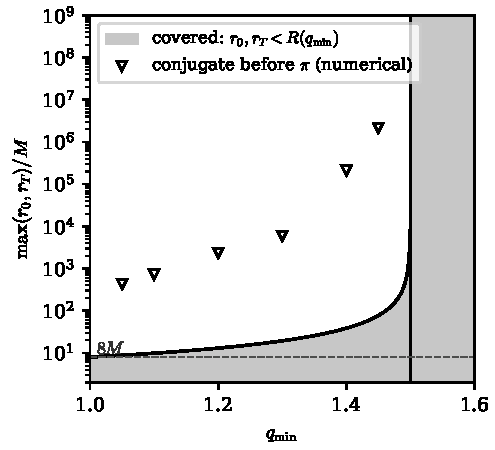
\includegraphics[width=0.6\textwidth]{../figures/fig2_radius.pdf}
\caption{Arrival branch, $a=0$. Theorem~\ref{thm:angle} covers $q_{\min}\ge3/2$ for an arbitrary
smooth factor. Below $3/2$, Theorem~\ref{thm:angle-radius} covers launch and target radii below $R(q_{\min})$ (shaded, logarithmic
scale), which exceeds $8M$ (dashed) for every $q_{\min}>1$ and diverges at $3/2$. Triangles: selected
numerical examples, for constant $A$, of in-plane conjugate points before $\pi$ (Remark~\ref{rmk:sharp32}),
plotted at $\max(r_0,r_T)$ with $r_T$ the radius of the zero; they do not mark the onset of failure.
The unshaded region is not covered by the radius estimate; failure at large radii is proved for
constant factors (Proposition~\ref{prop:sharp32}), and no sharp boundary is asserted.}
\label{fig:bands}
\end{figure}


\begin{remark}[what is new, and what is not covered]\label{rmk:angle-scope}
Theorem~\ref{thm:angle} holds for an arbitrary smooth conformal factor with $q\ge3/2$, with no
adiabatic assumption and no upper bound on $q$; for constant $A$ it strengthens the frozen
global-minimality statement of Paper~II to all competitors in three dimensions. The
convex-front argument in static conformal frames (supplementary material, sections~\ref{S-sec:frames}--\ref{S-sec:family}) is an
alternative proof on narrower ranges of $q$, where it also gives a stronger no-crossing
property. For $q<3/2$ somewhere, Theorem~\ref{thm:angle-radius} covers launch and
target radii below $R(q_{\min})$, in particular everything within $8M$ (Corollary~\ref{cor:within8M}).
Not covered by these swept-angle theorems: $q<3/2$ with launch or target beyond $R(q_{\min})$, where
the pointwise comparison of the two modes fails and, for constant $A$ at large radii, the rule
itself fails (Proposition~\ref{prop:sharp32}); small spin (Theorem~\ref{thm:D}) and persistence
(Theorem~\ref{thm:persistence}) cover some cases outside both theorems. Not covered at all: freezing; the spin $a\neq0$, where the drag of the seed adds a wind to the
front motion and the rotations about the launch axis are no longer isometries; and the
proper-time branch.
\end{remark}

% ======================================================================
\section{Persistence near constant data}
\label{sec:persistence}
% ======================================================================
Where the frozen problem is understood, its global minima survive a small change of the
conformal factor. The statement is qualitative.

\begin{theorem}[persistence, arrival branch]\label{thm:persistence}
Fix a launch event, two distinct spatial points and a compact time cylinder. Consider a
family of smooth, strongly convex rail indicatrices containing the origin uniformly,
depending on a parameter $A(\eta)$, and assume the uniform existence hypotheses of
Paper~I, Theorem~I.2, with a common competitor arriving with a strict time margin inside
the cylinder. Let the problem with $A\equiv A_0$ have a unique global minimum $\gamma_0$,
interior to the spatial region, such that the shooting map (initial direction, duration)
$\mapsto$ end point has invertible differential at $\gamma_0$. Then there is $\delta>0$ such
that for $\|A-A_0\|_{C^1}<\delta$ on the cylinder the arrival problem has a unique global
minimum in the region, the continuation of $\gamma_0$. The threshold $\delta$ depends on the
problem and on the cylinder.
\end{theorem}

\begin{proof}
Parametrize by $\eta$. With $B_A(\eta,x)=\{v:F_A(x,v,\eta)\le1\}$ the Hamiltonian is
$H_A=\max_{v\in B_A}\langle p,v\rangle$, for conformal Schwarzschild
$H_A=V_A|p|_{h_0^*}$; the flow $\dot x=\partial_pH_A$, $\dot p=-\partial_xH_A$ involves $A$
only through its value, and by homogeneity $|p(\eta_0)|=1$ may be imposed. Suppose
$A_k\to A_0$ with minimizers $\gamma_k$ different from the continued extremals. Theorem~I.2
gives existence; the common competitor and uniform coercivity give uniform bounds; a
subsequence converges in the convex body of velocities. For each fixed $\lambda<1$ sufficiently
close to one, slow the reference spatial trajectory by the factor $\lambda$: it lies strictly
inside the frozen velocity body, so it is admissible for the perturbed relaxed problem for
large $k$, and it arrives at $\eta_0+(T_0-\eta_0)/\lambda$; taking first $k\to\infty$ and then
$\lambda\uparrow1$ gives $\limsup T_k\le T_0$, while the limit reaches the target at a time $\ge T_0$. Hence
$T_k\to T_0$ and, by uniqueness, $\gamma_k\to\gamma_0$. For large $k$ the $\gamma_k$ are interior,
hence normal extremals (Theorem~I.2(ii)); their initial directions lie on a compact sphere
and every limit, together with $T_0$, generates $\gamma_0$, so by strong convexity the limit
direction is that of $\gamma_0$. The variational equations give convergence of the shooting
map and of its Jacobian, and the implicit function theorem gives a unique zero near that
of $\gamma_0$, which must be the data of $\gamma_k$: a contradiction.
\end{proof}

\begin{lemma}[persistence for a parameter family]\label{rmk:general-parameter}
Fix the launch, the spatial target and a compact regular time cylinder. Let $B_s(\eta,x)$ be a
uniformly coercive family of smooth, uniformly strongly convex velocity bodies, with the
origin uniformly in their interior. Assume a common competitor with a strict time margin,
existence and compactness of minimizers in a common region, and continuous dependence on $s$
of the bodies and of their support functions $H_s(\eta,x,p)$, including the $(x,p)$
derivatives needed for the Hamiltonian flow and its first variation away from $p=0$. If the
reference problem $s=0$, possibly non-autonomous, has a unique interior minimum with
invertible end-point shooting map, then for $s$ sufficiently close to $0$ there is a unique
global minimum in the common region, its continuation.
\end{lemma}

\begin{proof}
As for Theorem~\ref{thm:persistence}, which never uses that the reference is autonomous or
that the parameter is a conformal factor: the common competitor gives $\limsup$ of the
arrival times; closure in the convex body of velocities gives $\liminf$; uniqueness gives
convergence to the reference; interiority gives normality and normalized shooting data in a
compact set; the flow and strong convexity give convergence of those data; the invertible
Jacobian gives a local uniqueness that contains every perturbed minimum.
\end{proof}

\begin{remark}[quantifiers and the proper-time branch]
The order of quantifiers is ``for each frozen arc there is $\delta$''; no uniform $\delta$
over all arcs is claimed, and at $\Delta\varphi=\pi$ the frozen minimum is neither unique
nor non-degenerate. A slowly varying $A(\eta)=\bar A(\epsilon\eta)$ satisfies the $C^1$
condition on a fixed window, not on windows of length $O(\epsilon^{-1})$. The proper-time
problem requires a separate argument, because its cost differs from the arrival-time
functional. Section~\ref{sec:tau-var} establishes existence, absence of a relaxation gap and
perturbative global selection for $a=0$; finite variations of $A$ remain outside the
global-selection theorem.
\end{remark}

\begin{corollary}[near a constant factor]\label{cor:band}
Let $a=0$ and let $\gamma_0$ be an arrival extremal for a constant factor $A_0$ with
$q_0\ge3/2$ and $\Delta\varphi<\pi$. Then there is a $C^1$ neighborhood of $A_0$, depending
on $\gamma_0$, in which the continuation of $\gamma_0$ to the same target is the unique global
minimum among all rail curves.
\end{corollary}

\begin{proof}
Theorem~\ref{thm:angle} (for constant $A$ and $q\ge3/2$) gives uniqueness, and Lemmas~\ref{lem:tk-sturm}
and~\ref{lem:outofplane} give non-degeneracy before $\pi$ for a non-radial reference. For a radial reference,
Corollary~\ref{cor:radial} gives earliest arrival at every later event and no finite cut point, so no
finite conjugate point occurs. In the frozen problem the end-point shooting map is the exponential
map of the Fermat metric, parametrized by initial unit direction and length, and non-conjugacy
makes its differential invertible. Competitors that can
beat an arc of duration at most $T_{\rm up}$ satisfy $|\dd x/\dd\eta|_{h_0}\le1$ and stay in
the closed $h_0$-ball of radius $T_{\rm up}$, which is compact; take a regular region
containing it strictly. Theorem~\ref{thm:persistence} applies.
\end{proof}

\paragraph{Vaidya.} For ingoing Vaidya, the time reverse of Vaidya's radiating metric~\cite{Vaidya1951}, with frozen mass $m_0$,
$g=-f\,\dd v^2+2\,\dd v\,\dd r+r^2\dd\Omega^2$, $f=1-2m_0/r$, the Kodama
selector~\cite{Kodama1980,AbreuVisser2010} is $\partial_v=\partial_t$ with $v=t+r_*(r)$, $r_*'=1/f$, and the
rail charge is the Schwarzschild one. For a spatial tangent $\xi$ the arrival costs are
\begin{equation}
  F_t(\xi)=\frac{\Ehat}{\sqrt{\Ehat^2-f}}\sqrt{\frac{\xi_r^2}{f^2}+\frac{r^2}{f}|\xi_\Omega|^2},
  \qquad F_v(\xi)=F_t(\xi)+\frac{\xi_r}{f},
  \label{eq:vaidya-costs}
\end{equation}
so $\Delta v=\Delta t+r_*(r_f)-r_*(r_0)$: a fixed boundary term, which preserves the order of
all competitors. The frozen $v$-branch is therefore the Schwarzschild $t$-branch with
$q=\Ehat^2$, and its indicatrix is that of Paper~I. For a varying mass this is not a static
change of variables, and Theorem~\ref{thm:persistence} is applied directly to the Vaidya
support function with clock $v$ and parameter $m(v)$.

\begin{corollary}[Vaidya, arrival branch]\label{cor:vaidya}
Let $\Ehat^2\ge3/2$, $r_0,r_f>2m_0$, and let $\gamma_0$ be a frozen arrival extremal with
$\Delta\varphi<\pi$. Then every positive mass function $m(v)$ sufficiently close to $m_0$ in
$C^1$ on a common window admits a unique minimum of $v$ to the same target, the continuation
of $\gamma_0$, among all regular rail curves in $r>2m(v)$.
\end{corollary}

\begin{proof}
Frozen uniqueness and non-degeneracy come from Theorem~\ref{thm:angle} at constant mass, $q=\Ehat^2$. It remains to
confine the relevant competitors. With $w=\Ehat^2-f$, along every competitor
$\dd r/\dd v\le-w+\Ehat\sqrt w=f\sqrt w/(\Ehat+\sqrt w)<f/2\le1/2$, so none of duration at
most $T_{\rm up}$ goes beyond $r_0+T_{\rm up}/2$. For the inner side take
$2m_0<\rho<\min(r_0,r_f)$ and $|m-m_0|\le\epsilon_m$, $m_\pm=m_0\pm\epsilon_m$; in $r\ge\rho$,
$\dd r/\dd v\le\frac12(1-2m_-/r)$, so a competitor that dips below $\rho$ needs at least
\[
  L(\rho,r_f)=2(r_f-\rho)+4m_-\log\frac{r_f-2m_-}{\rho-2m_-}
\]
to climb back to $r_f$. At $\epsilon_m=0$ this bound diverges as $\rho\to2m_0$: choose first $\rho$
with $L>T_{\rm up}$ at $\epsilon_m=0$, then $\epsilon_m$ small enough to keep $L>T_{\rm up}$ and
$\rho>2m_+$ (at fixed $\epsilon_m>0$ the bound does not diverge). All relevant competitors then lie in a compact shell strictly outside
$2m(v)$, where $f>0$ and $w\ge\Ehat^2-1>0$ uniformly, and Theorem~\ref{thm:persistence}
applies.
\end{proof}

\begin{remark}
The radius of the neighborhood depends on the end points and the duration; it is not
uniform over Vaidya problems, and the result does not reach the region where the Kodama
selector stops being timelike. The arrival-time Fermat criterion does not certify minimality
of the proper-time functional, which is treated separately in section~\ref{sec:vaidya-tau}.
\end{remark}

% ======================================================================
\section{Ingoing Vaidya: the arrival branch}
\label{sec:vaidya-arrival}
% ======================================================================
Corollary~\ref{cor:vaidya} covers masses close to a constant. For every non-decreasing mass the
arrival branch is again a Fermat problem, and the results of sections~\ref{sec:schw}
and~\ref{sec:angle} carry over, with the mass in place of the conformal factor. With $w=\Ehat^2-f$, $f=1-2m(v)/r$ and $\Ehat>1$, define on
$D=\{(v,r,\Omega):v\in I,\ r>2m(v)\}$ the Lorentzian metric
\begin{equation}
  G=-w\,\dd v^2+\frac{(\dd r+w\,\dd v)^2}{\Ehat^2}+r^2\dd\Omega^2 .
  \label{eq:vaidya-G}
\end{equation}
For a curve parametrized by $v$, $G(1,s,\zeta)=-w+(s+w)^2/\Ehat^2+r^2|\zeta|^2$, so the future null
cone of $G$ is exactly the rail and its causal curves are the relaxed curves (the velocity body
$K$ of section~\ref{sec:vaidya-tau}); the $(v,r)$ block has determinant $-w/\Ehat^2<0$,
$G(\partial_v,\partial_v)=-wf/\Ehat^2<0$ in $D$, and $G^{-1}(\dd v,\dd v)=-1/w<0$, so $v$ is a temporal
function. The future null geodesics of $G$ are the arrival extremals, with $P_v=-h$ for the Vaidya
support function $h$. For constant mass, $v=t+r_*(r)$ gives
$G=(wf/\Ehat^2)\,[-\dd t^2+N h_0]$ with $N=\Ehat^2/w$, the auxiliary metric of
section~\ref{sec:schw} with $A=1$, up to a conformal factor. Equivalently, the normalized causal
velocities satisfy $(s+w)^2/\Ehat^2+r^2|\zeta|^2\le w$; the proper-time cost on this same velocity
body is treated separately in section~\ref{sec:vaidya-tau}.

\begin{theorem}[Vaidya arrival branch, non-decreasing mass]\label{thm:vaidya-arrival}
Let $\Ehat>1$ and let $m$ be smooth, positive and non-decreasing on an open interval $I$. Then
$(D,G)$ is globally hyperbolic. For every launch event $o$ and every spatial target $x_f\ne x_o$
reached by some future causal curve from $o$, the first arrival in $v$ is attained; every
first-arrival curve is a null pregeodesic of $G$; and a null geodesic $\gamma$ from $o$ is a first
arrival to the spatial point of $\gamma(\lambda)$, among all relaxed three-dimensional
competitors in $D$, exactly for $\lambda\le\lambda_c=\sup\{\lambda:\gamma(\lambda)\notin I^+(o)\}$.
If $\gamma(\lambda_c)$ is an interior event of $\gamma$, it is the first conjugate point or the first
point reached by a second maximal null geodesic, and before it the first arrival is unique up to
reparametrization.
\end{theorem}

\begin{proof}
A causal vector with $\dd v=0$ has $G=\dd r^2/\Ehat^2+r^2|\dd\Omega|^2\ge0$, so it vanishes: $v$
increases strictly along future causal curves and $(D,G)$ is causal. Let $q\in J^+(o)$ and let a
causal curve from $o$ to $q$ be parametrized by $v$. With $x=r-2m(v)$ and $s_+=-w+\Ehat\sqrt w$,
almost everywhere
$x'=s-2m'\le s_+\le f/2=x/(2r)\le x/(4m(v_o))$, using $m'\ge0$ twice and $\sqrt w\le\Ehat$; backward
integration gives $x\ge x_q\,e^{-(v_q-v)/(4m(v_o))}$, and $s\le1/2$ gives $r\le r_o+(v_q-v_o)/2$. Hence
$J^+(o)\cap J^-(q)$ lies in a compact subset of $D$. It is closed: for $z_n\to z$ in the diamond,
concatenate causal curves $o\to z_n\to q$; parametrized on $[v_o,v_q]$ they have uniformly bounded
velocities in that compact set, a subsequence converges uniformly to a causal curve from $o$ to
$q$ (closure of the cone through support functions), and it passes through $z$. Causality and
compact diamonds give global hyperbolicity~\cite{BernalSanchez2007}. If an arrival at $x_f$ occurs
at $v_q$, then $r_f>2m(v_q)\ge2m(v)$ for $v\le v_q$, so the line of $x_f$ is timelike on
$[v_o,v_q]$; Proposition~\ref{prop:first-arrival} applies with $\eta$ replaced by $v$.
\end{proof}

No closeness to constant mass and no limit of $m$ are assumed; the bound $m'\ge0$ is the null
energy condition of the ingoing dust. The theorem characterizes minimality by the cut point
without locating it: Corollary~\ref{cor:vaidya} places a prescribed target before the cut for
masses close to constant, and Theorem~\ref{thm:vaidya-antipodal-cut} below locates it at the
antipode for $\Ehat^2\ge3/2$. The construction is a specific instance of Fermat's principle in a
Lorentzian manifold~\cite{PerlickRayOptics}.

\begin{lemma}[antipodal bound]\label{lem:vaidya-antipode}
Rotations about the axis through the launch point are isometries of $G$. Along an equatorial
non-radial null geodesic they generate the Jacobi field $\varepsilon\, r\sin\varphi$ normal to the
plane, which vanishes at the launch and at $\varphi=\pi$. If a null geodesic reaches $\varphi=\pi$ in
$D$, that event is conjugate to $o$, and the cut point is not later.
\end{lemma}

\begin{theorem}[screen comparison]\label{thm:vaidya-sturm}
Let $\Ehat^2\ge3/2$ and let $m$ be smooth, positive and non-decreasing. Let $\gamma$ be a
future-directed non-radial null geodesic of $G$ starting at $o$, with positive swept angle
$\varphi$. There are no points conjugate to $o$ with $0<\varphi<\pi$. If $\gamma$ reaches $\varphi=\pi$
in $D$, that point is its first conjugate point and has screen multiplicity one.
\end{theorem}

\begin{proof}
Choose an affine parameter $\lambda$, an equatorial plane, and $L=r^2\varphi'>0$. The reflection
across the plane diagonalizes the tidal operator in a parallel screen frame
$(e_\perp,e_\parallel)$, $e_\perp=r^{-1}\partial_\theta$. With $K_i=R(e_i,k,e_i,k)$ and $k=\gamma'$,
$K_\perp+K_\parallel=\mathrm{Ric}(k,k)$, $K_\perp=L^2/r^4-r''/r$, and a direct computation gives
\[
  K_\perp-K_\parallel=\frac{L^2}{r^4(\Ehat^2r+2m-r)^2}
  \Big[\frac{mP(r)}{r}+m'\,r\big(3(\Ehat^2-1)r+4m\big)\Big],
\]
\[
  P(r)=3(2\Ehat^2-3)(\Ehat^2-1)r^2+(33\Ehat^2-38)mr+40m^2 .
\]
For $\Ehat^2\ge3/2$ every coefficient of $P$ is non-negative and the constant term is positive,
and $m'\ge0$: the right-hand side is positive. The normalized out-of-plane solution is
$u=(r_0/L)\,r\sin\varphi$, $u(0)=0$, $u'(0)=1$; let $z''+K_\parallel z=0$, $z(0)=0$, $z'(0)=1$. While
$u,z>0$, $(z'u-zu')'=(K_\perp-K_\parallel)uz>0$ and $(z/u)'=(z'u-zu')/u^2>0$; since $z/u\to1$ at the
launch, $z>u>0$ for $0<\varphi<\pi$, so the screen Jacobi determinant $uz$ does not vanish there.
If $\varphi=\pi$ is reached at $\lambda_\pi$ in $D$, then $u(\lambda_\pi)=0$, $u'(\lambda_\pi)=-r_0/r_\pi<0$, and
integrating the Wronskian identity gives $z(\lambda_\pi)>0$: only the out-of-plane mode vanishes.
\end{proof}

The threshold $\Ehat^2=3/2$ is that of Theorem~\ref{thm:angle}, where the same polynomial appears (Lemma~\ref{lem:tk-sturm}): the difference of the two modes is a Weyl component, and at constant mass the two metrics are conformal. Below it the
uniform comparison fails already for constant mass at large radii, and there, since at constant
mass the problem is conformal Schwarzschild with $q=\Ehat^2$, for $1<\Ehat^2<3/2$ there are in-plane conjugate
points before the antipode at large radii (Proposition~\ref{prop:sharp32}); the $m'$ term helps the sign of the comparison, which is not a
statement that accretion moves the cut point.

\begin{corollary}[strict local arrival minimality]\label{cor:vaidya-local-arrival}
Under the hypotheses of Theorem~\ref{thm:vaidya-sturm}, every compact segment with
$0<\varphi_T<\pi$ is a strict local minimizer of the arrival coordinate $v$ at the timelike receiver
of fixed spatial position through its endpoint, modulo orientation-preserving
reparametrization, among sufficiently close future-directed causal curves, with locality
understood for example in a fixed $C^1$ parametrization gauge.
\end{corollary}

\begin{proof}
On the screen the Dirichlet index form
$I(\eta,\eta)=\int_0^{\lambda_T}\sum_i(\eta_i'^2-K_i\eta_i^2)\,\dd\lambda$ is positive definite and
coercive on $H^1_0$ by Picone's identity, both fundamental solutions being positive on
$(0,\lambda_T]$. The arrival Hessian at the timelike receiver is $-I/G(k_T,\partial_v)$, with a
positive prefactor, and the local Fermat principle with a fixed reparametrization gauge gives
the claim for null competitors~\cite{GiannoniMasielloPiccioneFermat}; by spherical symmetry this
includes out-of-plane perturbations. The non-caustic null front defines a local causal barrier
in a sufficiently small tube about the segment, so nearby timelike competitors cannot arrive
earlier either.
\end{proof}

\paragraph{The cut at the antipode.} Conjugate points before $\pi$ are excluded; it remains to
exclude intersections of distinct earliest rays, with Proposition~\ref{prop:count}. Write $q=\Ehat^2$,
$w=q-1+2m(v)/r\in(q-1,q)$ in $D$, and
\[
  s_+(v,r)=-w+\sqrt{qw}=\frac{wf}{\sqrt{qw}+w},\qquad 0<s_+\le\frac f2\le\frac12 \quad\text{in } D .
\]
For a future causal curve parametrized by $v$ the cone gives $(\dd r/\dd v+w)^2/q\le w$, hence
$\dd r/\dd v\le s_+$. The radial null curves are $\dd r/\dd v=s_+$ (outgoing) and
$\dd r/\dd v=-w-\sqrt{qw}\le-(q-1)$ (ingoing), and at constant $r$ the curve with
$r^2(\dd\varphi/\dd v)^2=wf/q$ is null. A future causal vector with $\dd v=0$ vanishes, so along an
absolutely continuous curve whose velocity is future causal or zero almost everywhere, $v$ is
non-decreasing and $\dot r\le s_+\dot v$ almost everywhere.

\begin{theorem}[uniqueness in the planar cover]\label{thm:vaidya-cover-unique}
Let $\Ehat^2\ge3/2$, let $m$ be smooth, positive and non-decreasing on an open interval $I$, and
let $o=(v_0,r_0,0)$ lie in the universal cover $\widetilde D$ of the equatorial exterior. For every
$0<\delta<\pi$ there is at most one future null geodesic, up to reparametrization, from $o$ to the
partial receiver
\[
  \widetilde\Gamma=\{(v,r_T,\delta):\ v\in I,\ r_T>2m(v)\}.
\]
\end{theorem}

\begin{proof}
Suppose there are two, with arrivals $v_1\le v_2$. Then $r_T>2m(v_2)$; choose $b>v_2$ in $I$ with
$2m(b)<r_T$ and a smooth cutoff $0\le\chi\le1$ equal to one until after $v_2$ and zero for $v\ge b$.
Keep the mass before $v_2$ and set afterwards $\widetilde m(v)=m(v_2)+\int_{v_2}^v\chi(t)m'(t)\,\dd t$,
for all $v\ge v_2$, with $\chi m'$ extended by zero beyond $b$: a smooth, positive, non-decreasing mass on
$(\inf I,\infty)$, constant and equal to $m_\infty<r_T/2$ for $v\ge b$. Both rays are unchanged up to their
arrivals, and $\widetilde m\le m_\infty$ also before $v_0$, so the receiver is defined on all of $(\inf I,\infty)$.

With $\widetilde m$, Setting~(P) holds on $\widetilde D$ with $t=v$, $b=2\widetilde m$, $J=(\inf I,\infty)$,
$s_\pm=-w\pm\sqrt{qw}$ and $a=\sqrt{wf/q}/r$: the null cone is $(s+w)^2/q+r^2\zeta^2=w$, and $s_+\le1/2$. The
margin holds: $\sup b=2m_\infty<r_T$, $a(v,r_T)\ge\sqrt{(q-1)(1-2m_\infty/r_T)/q}/r_T$, and $s_-\le-(q-1)$. The
proof of Theorem~\ref{thm:vaidya-arrival} applies to $\widetilde m$; in the cover the angle is bounded on
diamonds as well, since $|\dd\varphi/\dd v|\le\sqrt w/r\le\Ehat/(2\widetilde m(v_a))$ along causal curves from any
event at $v=v_a$, so $\widetilde D$ is globally hyperbolic. The equatorial plane is totally geodesic, being the fixed set of a
reflection, so the null geodesics of $\widetilde D$ are the equatorial ones and their screen curvature
is $K_\parallel$. Along each of them $L=r^2\,\dd\varphi/\dd\lambda$ is conserved; $L=0$ gives $\varphi\equiv0\ne\delta$, so
$L\ne0$, $\varphi$ is strictly monotone and the swept angle is exactly $\delta\in(0,\pi)$. The proof of
Theorem~\ref{thm:vaidya-sturm} gives $z>0$ on $(0,\delta]$: every ray has index zero and a non-conjugate
end point. Proposition~\ref{prop:count} allows at most one, a contradiction.
\end{proof}

\paragraph{The direction of a ray.} The uniqueness proof does not need the following description
of the rays, which we record because it holds for every smooth positive mass. In a fixed plane,
with the orientation chosen so that $L>0$, a future null direction is described by an angle
$\alpha\in[0,\pi]$ through
\begin{equation}
  \frac{\dd r}{\dd v}=-w+\sqrt{qw}\cos\alpha,\qquad
  \frac{\dd\varphi}{\dd v}=\frac{\sqrt w}{r}\sin\alpha ,
  \label{eq:vaidya-alpha}
\end{equation}
$\alpha=0$ being the outgoing and $\alpha=\pi$ the ingoing radial direction. Here $q=\Ehat^2$ is the
case $A=1$; it is constant, unlike $\Ehat^2/A(\eta)^2$ in the conformal problem.

\begin{lemma}[direction equation]\label{lem:vaidya-direction}
Along a future non-radial null geodesic of $G$,
\[
  \frac{\dd\alpha}{\dd v}=\frac{\sin\alpha}{r}\,B(w,\cos\alpha),\qquad
  B(w,c)=c\,(2w-q+1)-\tfrac12\sqrt{q/w}\,(3w-q+1).
\]
The equation contains no $m'$ term; $B(q,1)=\tfrac12$ and
$B(q-1,c)=(q-1)c-\sqrt{q(q-1)}<0$ for $|c|\le1$.
\end{lemma}

\begin{proof}
Put $s=\dd r/\dd v$, $h=\dd v/\dd\lambda$ and $\dot w=2m'/r-2ms/r^2$, the total $v$-derivative of $w$
along the ray, and $\bar k=(1,s,\dd\varphi/\dd v)$. The connection of $G$ gives
\[
  \Gamma^v(\bar k,\bar k)=\frac{s}{r}+\frac{\dot w}{2w}+\frac{\cos\alpha}{r}\,B(w,\cos\alpha).
\]
Differentiating the conserved angular momentum $L=r\sqrt w\,h\sin\alpha$ and using
$h_v/h=-\Gamma^v(\bar k,\bar k)$, the term $\dot w/(2w)$, which carries $m'$, cancels against the
derivative of $\sqrt w$, and the stated equation follows where $\cos\alpha\ne0$; continuity gives it
also at $\cos\alpha=0$. (Equivalently, differentiate $\cos\alpha$ along the Hamiltonian flow of $G$ on
the null cone.)
\end{proof}


The accretion rate enters the direction only through the position of the ray, not explicitly;
in particular the outgoing radial direction is repelling near the boundary, where $B\to\frac12$,
and attracting at large radii, where $B<0$, for every mass profile.

\begin{theorem}[the arrival cut is at the antipode]\label{thm:vaidya-antipodal-cut}
Let $\Ehat^2\ge3/2$ and let $m$ be smooth, positive and non-decreasing. Every compact segment of
a future non-radial null geodesic of $G$ with swept angle in $(0,\pi)$ is the unique global
earliest arrival at its spatial end point, up to reparametrization, among all future causal
competitors in $D$, in three dimensions; in particular it is the unique minimum of $v$ among
all rail curves. If the geodesic reaches swept angle $\pi$ in $D$, that point is its first null
cut point.
\end{theorem}

\begin{proof}
By Theorem~\ref{thm:vaidya-arrival} an earliest arrival exists and is a null geodesic. By
spherical symmetry it lies in the plane through the center, the launch and the target; it
cannot have swept angle above $\pi$, since the antipodal conjugate point of
Lemma~\ref{lem:vaidya-antipode} would be interior, nor equal to $\pi$; so it is in the same short
lifted class as the given segment, and Theorem~\ref{thm:vaidya-cover-unique} identifies the two.
If the antipodal event, when reached in $D$, were in $I^+(o)$, openness of $I^+(o)$ would put
preceding points of the same ray there as well, contradicting their earliest-arrival property;
the rotations of the plane give distinct earliest rays, and beyond it the conjugate point is
interior.
\end{proof}

This is the analogue of Theorem~\ref{thm:angle} for every non-decreasing mass, with no
closeness to constant mass, no bound on the accretion rate and no limit of $m$. The step that
does not transfer from the static case, the convexity of the fronts, is replaced by the
count of Proposition~\ref{prop:count}, in which the moving boundary enters only through the
truncation of the mass and the margin of the receiver. As an illustration only, non-certified root searches with $\Ehat^2=2$,
$r_0=6$ and $r_T\in\{6,10\}$ found one same-sense ray for each sampled lifted angle in
$[0.02\pi,1.9\pi]$ for constant mass, $m=1+\frac12\tanh(v/5)$ and a jump of $m$ from $1$ to $2$ within
$\Delta v\approx0.6$; the search does not certify completeness, and the observations beyond $\pi$
are not conclusions of the theorem.

\paragraph{Below $\Ehat^2=3/2$: a radius bound.} As for conformal Schwarzschild
(Theorem~\ref{thm:angle-radius}), the comparison of Theorem~\ref{thm:vaidya-sturm} survives near the center,
and it suffices that the rays reaching a receiver do not go far out. Here, unlike the conformal case,
accretion can turn an outgoing ray back, because the velocity body moves with the mass; a bound on the
accretion rate excludes this. Write $q=\Ehat^2$, $f=1-2m/r$ and $\widehat R(q)=R(q)/M$, with $R$ from
Lemma~\ref{lem:radius}.

\begin{lemma}[no return beyond $3m$]\label{lem:vaidya-no-return}
Let $1<q<3/2$ and let $m$ be smooth, positive and non-decreasing with
\[
  m'<\mu_*(q):=\min\Big\{\frac1{27q},\frac{q-1}q\Big\}.
\]
At every point of a future null geodesic of $G$ where $\dd r/\dd v=0$ and $r\ge3m(v)$, one has
$\dd^2r/\dd v^2>0$. Consequently a segment with radial end points $r_0$, $r_T$ satisfies
$r\le\max\{r_0,r_T,3\sup m\}$.
\end{lemma}

\begin{proof}
By~\eqref{eq:vaidya-alpha} and Lemma~\ref{lem:vaidya-direction}, at a turning point $\cos\alpha=\sqrt{w/q}$ and the
total derivative of $w$ along the ray is $2m'/r$, so
\[
  \frac{\dd^2r}{\dd v^2}=-\frac1r\Big[m'+\Big(1-\frac wq\Big)Q(w)\Big],\qquad
  Q(w)=2w^2-\Big(\frac{5q}2-1\Big)w+\frac{q(q-1)}2 ,
\]
since $\sqrt{qw}\,B(w,\sqrt{w/q})=Q(w)$. With $w=q-f$ and $1/3\le f<1$ for $r\ge3m$, the function
$g_q(f)=-(1-w/q)Q(w)=-2f^3/q+(3/2+1/q)f^2-f/2$ satisfies
\[
  g_q(f)=\tfrac32(1-f)\frac1{27q}+\tfrac32\Big(f-\frac13\Big)\frac{q-1}q
  +\frac{(f-\frac13)(1-f)(12f+10-9q)}{6q}\ \ge\ \mu_*(q),
\]
because the first two weights are non-negative with sum one and $12f+10-9q>1/2$. Hence
$\dd^2r/\dd v^2=(g_q(f)-m')/r>0$. If a segment exceeded $\max\{r_0,r_T,3\sup m\}$, the radius would have an
interior maximum there, with $\dd r/\dd v=0$, $\dd^2r/\dd v^2\le0$ and $r>3m(v)$: a contradiction. No
assumption on the number of turning points is needed.
\end{proof}

\begin{theorem}[radius bound below $3/2$]\label{thm:vaidya-radius}
Let $1<\Ehat^2<3/2$ and let $m$ be smooth and non-decreasing on an open interval $I$, with
$0<m_0\le m\le m_{\max}$ and $m'<\mu_*(\Ehat^2)$. Let a non-radial future null geodesic of $G$ be launched at
$o=(v_0,r_0,\Omega_0)$, and consider its events at radius $r_T$, with the segment in $D$. If
\[
  \max\{r_0,r_T,3m_{\max}\}<\widehat R(\Ehat^2)\,m_0,
\]
the segment is a global earliest arrival in $v$ among all relaxed three-dimensional competitors, in
particular among all rail curves, if and only if its swept angle is at most $\pi$; for an angle below $\pi$
it is unique up to reparametrization; if the angle $\pi$ is reached in $D$, that event is the first null
cut point and the first conjugate point, of screen multiplicity one; beyond it the segment is not
minimizing. The bound on $m'$ is sufficient; it is not asserted to be necessary or sharp.
\end{theorem}

\begin{proof}
\emph{Comparison.} The identity for $K_\perp-K_\parallel$ in the proof of Theorem~\ref{thm:vaidya-sturm} holds for every
$q>1$, with $P(r;m)=m^2P_q(r/m)$ and $P_q$ the polynomial of Lemma~\ref{lem:radius} at $M=1$. Along every
ray with radial end points $r_0$, $r_T$, Lemma~\ref{lem:vaidya-no-return} and $m\ge m_0$ give
$r\le\max\{r_0,r_T,3m_{\max}\}<\widehat R(q)m_0\le\widehat R(q)m(v)$, so $P(r;m(v))>0$ pointwise; the $m'$ term is
non-negative. The Wronskian argument of Theorem~\ref{thm:vaidya-sturm} then excludes conjugate points before
$\pi$ and gives multiplicity one at $\pi$.

\emph{Uniqueness in the cover.} Suppose two rays reach the receiver $(v,r_T,\delta)$, $0<\delta<\pi$, at
$v_1\le v_2$. Truncate the mass after $v_2$ as in Theorem~\ref{thm:vaidya-cover-unique}; the new mass
$\widetilde m$ keeps $m_0\le\widetilde m\le m_{\max}$ and $0\le\widetilde m'=\chi m'<\mu_*(q)$. Every ray of the cover from the
launch to the receiver, including those arriving after $v_2$, has radial end points $r_0$, $r_T$, so the
previous step applies to all of them: index zero and non-conjugate end point. The other hypotheses of
Setting~(P), the margin of the receiver and global hyperbolicity use only $q>1$, as in the proof of
Theorem~\ref{thm:vaidya-cover-unique}; Proposition~\ref{prop:count} allows at most one ray.

\emph{Three dimensions and the cut.} As in Theorem~\ref{thm:vaidya-antipodal-cut}: an earliest arrival exists, is
planar and lies in the short class, so it is the given segment. Before an event at angle $\pi$ all
points have radius at most $\max\{r_0,r_T,3m_{\max}\}$ and are earliest arrivals; openness of $I^+(o)$ and the
rotations of the plane make the antipodal event the first cut point, and beyond it the out-of-plane
conjugate point is interior.
\end{proof}

\begin{corollary}[within $8m_0$]\label{cor:vaidya-8m}
Under the regularity, mass and accretion-rate assumptions of Theorem~\ref{thm:vaidya-radius}, if $m_{\max}\le\frac83m_0$, the
conclusions hold for every non-radial segment with launch and target radii $r_0,r_T\le8m_0$ in $D$.
\end{corollary}

\begin{proof}
$\widehat R(q)>8$ for every $q>1$, so $\max\{r_0,r_T,3m_{\max}\}\le8m_0<\widehat R(q)m_0$.
\end{proof}

The same holds on a finite window $[v_0,T]$, provided $m$ is smooth and non-decreasing on an open
neighborhood of it, with the bounds there and a slightly larger $\bar m_{\max}$ still satisfying the radius
condition. Choose a short interval after $T$ on which $0\le m'<\mu_*(q)$, $m\le\bar m_{\max}$ and $2m<r_T$, and a smooth cutoff
$\chi$, equal to one near $T$ and to zero afterwards; set $\widetilde m(v)=m(T)+\int_T^v\chi(s)m'(s)\,\dd s$ for $v\ge T$,
keeping $m$ unchanged up to $T$, as in the truncation of Theorem~\ref{thm:vaidya-cover-unique}. This preserves
monotonicity and the rate bound, and competitors arriving no later than $T$ meet only the unchanged
profile. One-sided monotonicity up to $T$ is not enough for this extension. The threshold $\mu_*$ equals $(q-1)/q$ for $q\le28/27$ and $1/(27q)$ above,
with maximum $1/28$ and $\mu_*\to0$ as $q\to1^+$. It is the best uniform lower bound of $g_q$ on $r\ge3m$; above it the
equations admit local apoastra. Whether the cut rule still holds under the stated radius restriction when
the accretion-rate bound is removed remains open.

\paragraph{Decreasing mass.} In the ingoing Vaidya convention, a decreasing $m(v)$ corresponds to
an ingoing negative-energy flux and violates the null energy condition; the profiles considered
here may be viewed as effective evaporation models, rather than classical positive-energy
accretion. The argument above used $m'\ge0$ only for global hyperbolicity and for the sign of the
accretion term in the comparison. Both have quantitative replacements, at the price of a domain
with a timelike boundary. The metric~\eqref{eq:vaidya-G} is Lorentzian on the whole ambient
$\{r>0\}$, where $w=q-1+2m/r>0$, the $(v,r)$ block has determinant $-w/q$ and $v$ remains a time
function; the competitors live in $\Lambda=\{r>2m(v)\}$. Set
\begin{gather*}
  F(v)=-2m''+\frac{m'+(4+5/q)\,m'^2+4(1+q)\,m'^3/q^2}{m},\\
  H_q(z)=\frac{z\,[3(2q-3)(q-1)+(33q-38)z+40z^2]}{3(q-1)+4z},
\end{gather*}
and, for a launch $o=(v_0,r_0,\Omega_0)$, $R(v)=r_0+(v-v_0)/2$.

\paragraph{Hypothesis (H$_{\rm dec}$).} $q=\Ehat^2\ge3/2$; $m\in C^\infty(\mathbb R)$ is positive with
$-q<m'<0$ and $F\le0$ everywhere; $-m'(v)\le H_q\big(m(v)/R(v)\big)$ for $v\ge v_0$; the launch has
$r_0>2m(v_0)$, and the receiver radius satisfies $r_T>2\sup m$.

\begin{lemma}[the boundary]\label{lem:vaidya-dec-boundary}
Under (H$_{\rm dec}$) the boundary $r=2m(v)$ of $\Lambda$ is smooth and timelike, and $\Lambda$ is light-convex: a
null geodesic of the ambient metric contained in $\bar\Lambda$ with end points in $\Lambda$ lies in $\Lambda$.
\end{lemma}

\begin{proof}
With $X=\partial_v+2m'\partial_r$, tangent to the boundary, $G(X,X)=4m'(1+m'/q)<0$. For a null vector $k$
tangent to the boundary, $k^r=2m'k^v$ and $(2m)^2|k^\Omega|^2=-4m'(1+m'/q)(k^v)^2$, and a direct
computation gives $\mathrm{Hess}_G(r-2m)(k,k)=(k^v)^2F(v)\le0$. Let a null geodesic in $\bar\Lambda$ touch the
boundary at an interior parameter; parametrize it by $v$ and put $u=r-2m(v)\ge0$, with $u=u'=0$ at
the contact. Eliminating the angular velocity with the null condition, which is regular there
because $-4m'(1+m'/q)>0$, the radial equation reads $u''=F+E$ with $|E|\le C(|u|+|u'|)$, so
$u''\le C(u+|u'|)$. Gr\"onwall applied to $(u')_+$ and $u$, forwards and backwards, gives $u\equiv0$
near the contact; the set of contacts is open and closed along the geodesic, which would then lie
on the boundary, contradicting its end points.
\end{proof}

\begin{lemma}[strict comparison]\label{lem:vaidya-dec-sturm}
Under (H$_{\rm dec}$), along every future causal curve from $o$, $r(v)<R(v)$ for $v>v_0$, and along every
non-radial null geodesic from $o$ in $\Lambda$, $K_\perp-K_\parallel>0$. In particular, in the plane of such a
geodesic the in-plane mode has no zero on $(0,\pi]$: within the plane, no point with swept angle
in $(0,\pi]$ is conjugate to $o$.
\end{lemma}

\begin{proof}
Along a causal curve, $\dd r/\dd v\le s_+=wf/(\sqrt{qw}+w)<f/2<\frac12$, since $w<q$ and $0<f<1$; so
$r(v)<R(v)$. For $q\ge3/2$, $H_q$ is strictly increasing on $z>0$: with $c_0=3(2q-3)(q-1)\ge0$, $c_1=33q-38>0$ and
$c_2=3(q-1)>0$, the numerator of $H_q'$ is $c_0c_2+2c_1c_2z+(4c_1+120c_2)z^2+320z^3>0$; hence
$m'+H_q(m/r)>m'+H_q(m/R)\ge0$, and the formula in the proof of Theorem~\ref{thm:vaidya-sturm}
writes $K_\perp-K_\parallel$ as a positive multiple of $m'+H_q(m/r)$: indeed
$mP(r)/r+m'r(3(q-1)r+4m)=r(3(q-1)r+4m)\,[m'+H_q(m/r)]$. With $u$ and $z$ as there, $W=z'u-zu'$ has
$W'=(K_\perp-K_\parallel)uz>0$ while $u,z>0$, so $z>u>0$ before $\varphi=\pi$; at $\varphi=\pi$, $u=0$ and $W>0$
give $z>0$.
\end{proof}

\begin{lemma}[null polygons]\label{lem:null-polygon}
Let $\Lambda$ be an open subset of a stably causal Lorentzian manifold of dimension at least two and
$c:[0,1]\to\Lambda$ a future causal curve. There is a future null broken geodesic in $\Lambda$ with the same end
points; in particular it admits an $H^1$ parametrization.
\end{lemma}

\begin{proof}
For each point of the compact image of $c$ choose a convex normal neighborhood $W$ with closure in $\Lambda$,
carrying a local time function $t$, and a smaller neighborhood $U$ with closure in $W$ such that every
future null geodesic from a point of $U$ can be continued inside $W$ at least up to the largest
value of $t$ on $U$; this is possible because null vectors normalized by $\dd t=1$ have uniformly
bounded spatial components on compact charts. By compactness and continuity, split $c$ at points
$p_0,\dots,p_n$ so that each subarc is contained in a common $U$; its end points are then causally related
within $W$. Below, $I^-_W$ and $J^-_W$ denote the chronological and causal pasts relative to $W$. If $p_i=p_{i+1}$, drop the piece; if they are null-related in $W$, use the null
segment. If $p_i\ll p_{i+1}$ in $W$, follow a future null geodesic from $p_i$ in $W$: it starts in $I^-_W(p_{i+1})$, it
does not pass through $p_{i+1}$ (otherwise the two points would be null-related in $W$), and at the level
$t(p_{i+1})$ it is at a point different from $p_{i+1}$, hence outside $J^-_W(p_{i+1})$. Its first crossing of
$\partial I^-_W(p_{i+1})$ is a point $e$ null-related to $p_{i+1}$ in $W$, and $p_ie$, $ep_{i+1}$ are null segments in $W$.
Concatenate.
\end{proof}

\begin{proposition}[one ray per class, decreasing mass]\label{prop:vaidya-dec-count}
Assume (H$_{\rm dec}$) and work in the universal cover $\tilde\Lambda$ of the equatorial domain, with the receiver
$\gamma(v)=(v,r_T,\Theta)$, $v\in\mathbb R$, $0<|\Theta|\le\pi$. Then there is exactly one future null geodesic from $o$ to
$\gamma$ in $\tilde\Lambda$, and it is the unique earliest arrival among all future causal curves in $\tilde\Lambda$ from
$o$ to $\gamma$.
\end{proposition}

\begin{proof}
\emph{Hypotheses of~\cite[Theorem~1.7]{GiannoniMasielloPiccioneMorse}.} The ambient
$\mathbb R_v\times(0,\infty)\times\mathbb R_\varphi$ is stably causal, $v$ being a time function. By
Lemma~\ref{lem:vaidya-dec-boundary} the boundary of $\tilde\Lambda$ is smooth, timelike and light-convex. The
receiver is timelike, since $G(\partial_v,\partial_v)=-wf/q<0$ at $r_T>2\sup m$, and a closed embedding; $o$ is not
on it. Sublevels of arrival at most $c\ge v_0$ lie in the compact subset
$K(c)=\big([v_0,c]\times[2m_{\min}(c),R(c)]\times[-\Phi_c,\Phi_c]\big)\cap\{r\ge2m(v)\}$ of the closure, with
$m_{\min}(c)=\min_{[v_0,c]}m$ and $\Phi_c=\sqrt q\,(c-v_0)/(2m_{\min}(c))$, by $\dd r/\dd v<\frac12$ and
$|\dd\varphi/\dd v|\le\sqrt w/r$; for $c<v_0$ they are empty. Precompactness in the closure is what GMP
require~\cite[Definition~1.2]{GiannoniMasielloPiccioneMorse}.
The space $\mathcal L^+$ is not empty: a radial null segment from $o$ to $r=r_T$, outgoing with
$\dd r/\dd v=s_+$ bounded below on $[r_0,r_T]$ since $m\le m(v_0)$ there, or ingoing, followed by the null
curve at $r=r_T$ with $|\dd\varphi/\dd v|=\sqrt{wf/q}/r_T$, bounded below because $r_T>2\sup m$. Every future null
geodesic from $o$ to $\gamma$ has swept angle exactly $|\Theta|$ (its angular momentum is conserved, and
$L=0$ cannot reach $\Theta\ne0$), so by Lemma~\ref{lem:vaidya-dec-sturm} it has index zero and a non-conjugate
end point.

\emph{Count.} Setting~(P) holds with $t=v$, $b=2m$, $s_\pm=-w\pm\sqrt{qw}$ and $a=\sqrt{wf/q}/r$, with the margin
$\sup b=2\sup m<r_T$, $a(v,r_T)\ge\sqrt{(q-1)f_*/q}/r_T$ with $f_*=1-2\sup m/r_T>0$, and
$s_-\le-(q-1)-\sqrt{q(q-1)}<0$ on $r\ge r_T$. We reuse only the tail construction, its $H^1$ continuity and
the contraction in the proof of Proposition~\ref{prop:count}; these do not use global hyperbolicity.
The outgoing tail from an event of a curve in $\tilde\Lambda$ stays above that curve by
Lemma~\ref{lem:outermost}, hence in $\tilde\Lambda$, and the ingoing and angular tails stay in $r\ge r_T>2\sup m$;
continuity is local on the compact images, not uniform up to the boundary. So $\mathcal L^+$ is
contractible, and the algebraic count at the end of that proof gives exactly one null geodesic
$\gamma_\Theta$. Non-emptiness was proved above and compactness by $K(c)$; earliest arrival is obtained
separately below.

\emph{Earliest arrival.} Let $T$ be the time function of~\cite{GiannoniMasielloPiccioneMorse} and
$Q(z)=\int_0^1(\dd(T\circ z)/\dd s)^2\dd s$, with $T$ the time function chosen there. A curve of $\mathcal L^+$ arriving at
$\gamma(a)$ satisfies $Q(z)\ge[T(\gamma(a))-T(o)]^2$, with equality when $T\circ z$ is affine, and $T\circ\gamma$ is
increasing. Reparametrize $\gamma_\Theta$ on $[0,1]$ so that $T\circ\gamma_\Theta$ is affine: it then represents the unique
critical point of $Q$, with value $[T(\gamma(a_\Theta))-T(o)]^2$, $\gamma(a_\Theta)$ being its arrival. If a causal curve
in $\tilde\Lambda$ arrived before $\gamma_\Theta$, Lemma~\ref{lem:null-polygon} would give a null broken geodesic $z$ with the
same arrival $a<a_\Theta$, which after reparametrization with $T\circ z$ affine has $Q(z)<Q(\gamma_\Theta)$. For
$Q(z)<b<Q(\gamma_\Theta)$, $b$ is not a critical value, since the only critical value exceeds it, and the sublevel
$\mathcal L^+\cap Q^b$ is not empty, so its zeroth Betti number is at least one; in the Morse relations on
sublevels~\cite[Theorem~7.1]{GiannoniMasielloPiccioneMorse}, proved in the same setting with boundary, the
constant term gives (number of critical points of index zero below $b$) $=b_0+s_0\ge1$, while the left
side is zero, a contradiction. Finally, a causal curve arriving at the same time as $\gamma_\Theta$ is a null pregeodesic,
otherwise local push-up and the timelike receiver would give an earlier arrival, so it is $\gamma_\Theta$.
\end{proof}

\begin{lemma}[angular reduction]\label{lem:vaidya-reduction}
Let $z=(v,r,\Omega)$ be a future causal curve in $\Lambda$ from $o$, absolutely continuous, and
$\theta=d_{S^2}(\Omega,\Omega_0)\in[0,\pi]$. The planar curve $\bar z=(v,r,\theta)$, in a fixed plane through the center and
$\Omega_0$, is future causal, lies in $\Lambda$, arrives at angular distance $\theta$ at the same value of $v$, and its
lifted angle stays in $[0,\pi]$.
\end{lemma}

\begin{proof}
The distance to $\Omega_0$ is $1$-Lipschitz on the sphere, so $\theta$ is absolutely continuous with
$|\theta'|\le|\Omega'|$ almost everywhere, also where $z$ passes through $\Omega_0$ or its antipode. The cone
$(r'+wv')^2/q+r^2|\Omega'|^2\le wv'^2$ depends on the angular motion only through $|\Omega'|$, and $v,r$ are
unchanged.
\end{proof}

\begin{theorem}[the arrival cut for decreasing mass]\label{thm:vaidya-dec}
Assume (H$_{\rm dec}$) and $\Ehat>0$, and fix a target at radius $r_T>2\sup m$. Let $\gamma$ be a non-radial future null
geodesic of $G$ from $o$ to that target, contained in $\Lambda$, with terminal swept angle $\delta$.
\begin{enumerate}
\item If $\delta\in(0,\pi)$, $\gamma$ is the unique global earliest arrival at the target, up to
  reparametrization, among all future causal competitors in $\Lambda$, in three dimensions.
\item If $\delta=\pi$, $\gamma$ is an earliest arrival at the target, not unique, and the target event is its
  first cut point.
\end{enumerate}
Moreover, every segment of a non-radial null geodesic from $o$ contained in $\Lambda$ with swept angle
greater than $\pi$ is not minimizing, whatever the radius of its end point.
\end{theorem}

\begin{proof}
Use the plane through the center, $\Omega_0$ and the target. By Lemma~\ref{lem:vaidya-reduction} every 3D competitor
reduces to a planar causal curve in the class $\Theta=\delta$ with the same arrival, so by
Proposition~\ref{prop:vaidya-dec-count} no competitor arrives before $\gamma_\delta$, the planar ray of that class,
which is therefore a 3D earliest arrival; $\gamma=\gamma_\delta$ by uniqueness in the class. For $\delta<\pi$, let $z$ be a 3D
earliest arrival: then $\bar z$ is a planar one, hence $\bar z=\gamma_\delta$, whose angle is monotone; since $\bar z$ is
null, the cone inequality for $z$ forces $|\Omega'|=|\theta'|$ almost everywhere, so the projection of $z$ to the
sphere has length $\delta$ and is the unique minimizing arc, and $z=\gamma_\delta$. For $\delta=\pi$, the rotations about
the axis through the center and $\Omega_0$ give a family of distinct earliest arrivals. No earlier event
of $\gamma$ is a cut point: a chronological advantage at a prefix would propagate to the target by
push-up, and a second maximal segment to an earlier event, concatenated with the tail of $\gamma$,
would create a corner that push-up improves, unless the tangents coincide, which by uniqueness
of geodesics would make the two segments equal. So the target event is the first cut point.
Beyond $\pi$ the out-of-plane Jacobi field generated by the rotations, proportional to $r\sin\varphi$ in the
plane, has an interior zero; a variation inside a compact neighborhood of the segment contained
in $\Lambda$ gives a timelike connection to the end point, and the static line through the end point,
timelike near it since $f>0$, yields an earlier arrival. This last step is local and needs no
margin on the radius of the end point.
\end{proof}

\paragraph{An admissible profile.} Let $q\in\{3/2,2\}$, $m(v)=1+\frac15\big/\big(1+e^{(v-5)/5}\big)$ (units with
$m_\infty=1$), $v_0=0$, $r_0=6$, $r_T>12/5$. With $s=1/(1+e^{(v-5)/5})$, $-m'=d=\frac1{25}s(1-s)\le\frac1{100}$ and
$|m''|\le\frac15d$, so $-q<m'<0$, and the bracket in $F$ is at most $-d(1-(4+5/q)d)\le-d/2$; hence
$F\le(\frac25-\frac5{12})d<0$. For Sturm, $d\le e^{1-v/5}/25$ and $R=6+v/2$. Since
$H_2(z)=z+z^2(24+40z)/(3+4z)\ge z$ and $Re^{-v/5}$ decreases for $v\ge0$, $Rd\le6e/25<1\le m$, so
$d<H_2(m/R)$. Since $H_{3/2}(z)=\frac{23}3z^2+\frac{28}3z^3/(\frac32+4z)\ge\frac{23}3z^2$ and $R^2e^{-v/5}$ decreases,
$R^2d\le36e/25<\frac{23}3\le\frac{23}3m^2$, so $d<H_{3/2}(m/R)$. Hypothesis (H$_{\rm dec}$) holds on the whole
future, at the threshold $q=3/2$ as well. For $q>3/2$ the bound $H_q(z)\ge(2q-3)z$ gives more room; for a
fixed profile the admissible launch radii are bounded, but a smaller amplitude admits any finite
$r_0$.

The statement concerns null geodesics of $G$, the arrival extremals, not arbitrary rail curves, and
it requires the margin $r_T>2\sup m$ on the receiver. A mass that becomes exactly constant makes the
boundary null in the future and is not covered by this argument; neither is a mass whose
derivative changes sign, where the boundary is partly spacelike.

% ======================================================================
\section{Conformal Kerr: a barrier, and small spin}
\label{sec:kerr}
% ======================================================================
For $a\neq0$ the exterior $r>2M$ is not globally hyperbolic for $\gopt$: $\Delta(2M)=a^2$, so
$r=2M$ lies at finite $h_0$-distance, the Randers condition degenerates there,
$|\beta|_{h_0}\to1$, and $N\to1$. Causal curves reach $r=2M$ in finite $\eta$, consistently
with Paper~II, where the compact-control problem ends at $r=2M$. We show that fast
competitors cannot get there.

\paragraph{Hypothesis (H2).} $0<|a|\le M$, $\Ehat>0$, $A\in C^\infty(I)$ positive with
$\sup_IA<\Ehat$ (no freezing on $r>2M$).

\subsection{The cost of an excursion}
Let
\begin{equation}
  \theta(r)=1-\frac{2M|a|}{r\sqrt\Delta},\qquad
  c(r)=\theta(r)\sqrt{P_0(r)}=\theta(r)\frac{r}{\sqrt{f\Delta}},\qquad
  C(r_1,r_2)=\int_{r_1}^{r_2}c(r)\,\dd r ,
  \label{eq:excursion}
\end{equation}
with $f=1-2M/r$ and $P_0=h_{0,rr}$ at the equator. $\theta$ increases, since $r^2\Delta$ does, from $0$ at $r=2M$ to
$1$, and $C(r_1,r_2)$ stays finite as $r_1\to2M^+$ when $a\neq0$.

\begin{lemma}[the equator is the worst latitude]\label{lem:worst}
For $r>2M$ and $|a|\le M$, the function $F(r,\vartheta)=(1-|\beta|_{h_0})\sqrt{h_{0,rr}}$ is,
at fixed $r$, minimal at the equator, where it equals $c(r)$; it is non-increasing in
$\sin\vartheta$, strictly if $a\ne0$.
\end{lemma}

\begin{proof}
With $x=\sin\vartheta$, $\Sigma=r^2+a^2-a^2x^2$ and $k=2M|a|r/\sqrt\Delta$ one has
$|\beta|_{h_0}=kx/\Sigma$ and $\sqrt\Delta\,F=G(x)=(\Sigma-kx)/\sqrt{\Sigma-2Mr}$, with
$(\Sigma-2Mr)^{3/2}G'(x)=a^2x(4Mr-\Sigma)-k\Delta$. If $4Mr\le\Sigma$ this is negative.
Otherwise $\Sigma\ge r^2$ and $x\le1$ give $a^2x(4Mr-\Sigma)\le a^2r(4M-r)$, and it remains to
show $|a|(4M-r)<2M\sqrt\Delta$ for $2M<r<4M$: with $r=2M+s$,
$4M^2\Delta-a^2(4M-r)^2=s(8M^3+4Ma^2)+s^2(4M^2-a^2)>0$.
\end{proof}

\begin{lemma}[excursion cost]\label{lem:excursion}
A causal curve that starts at $r\ge r_2$, reaches $r\le r_1$ and returns to $r\ge r_2$ uses a
conformal time at least $2C(r_1,r_2)$, at any latitude and with any polar motion.
\end{lemma}

\begin{proof}
For a future causal vector, $N\ge1$ and Lemma~\ref{lem:gopt-basic} give
$v^\eta\ge(1-|\beta|_{h_0})|v_x|_{h_0}\ge F(r,\vartheta)|v^r|\ge c(r)|v^r|$ by
Lemma~\ref{lem:worst}. With $B'=c$, $\int c(r)|r'|\ge|B(r_{\rm end})-B(r_{\rm start})|$; apply
it to each of the two crossings of $[r_1,r_2]$. This is a total-variation bound: no
monotone pieces are needed.
\end{proof}

\subsection{First arrival within the margin}
\begin{theorem}[conformal Kerr within the margin]\label{thm:kerr}
Assume (H2), $2M<r_1<r_2$, a launch event $o$ at $r_0\ge r_2$ and a target $x_f$ with
$r_f\ge r_2$, and a rail curve from $o$ to $x_f$ of duration $T_{\rm up}<2C(r_1,r_2)$ with
$[\eta_0,\eta_0+T_{\rm up}]\subset I$. Then every rail curve from $o$ reaching $x_f$ within
$T_{\rm up}$ stays in $r>r_1$; a first-arrival rail curve to $x_f$ exists and is a null
pregeodesic of $\gopt$ with no interior conjugate point. Moreover, let $\gamma$ be a rail
extremal from $o$ whose end point lies in $r\ge r_2$ and whose elapsed duration is at most
$T_{\rm up}$. For this segment and its prefixes, first arrival is characterized by the null
cut point in the confined problem: the segment is globally minimal among all
three-dimensional competitors precisely up to that point, the first conjugate point or the
first meeting with another minimizing null geodesic from $o$, and the minimum is unique
before it.
\end{theorem}

\begin{proof}
Choose $\delta>0$ with $T_{\rm up}<2C(r_1+\delta,r_2)$ and a smooth $\psi\ge1$ on $(r_1,\infty)$,
equal to $1$ for $r\ge r_1+\delta$, with $\int_{r_1}\sqrt{\psi P_0}\,\dd r=+\infty$, and replace
$h_0$ by $h_0^\psi$ (radial part multiplied by $\psi$). The cones of the modified metric
$\tilde g$ lie inside those of $\gopt$, and the two metrics coincide on $r\ge r_1+\delta$. With
$b_1=2M|a|/(r_1\sqrt{\Delta(r_1)})<1$ the slice metric is $\ge(1-b_1^2)h_0^\psi$, complete on
$(r_1,\infty)\times S^2$; the lapse lies between $1$ and $(1-b_1^2)^{-1/2}$ and the shift is
bounded by $b_1/(1-b_1^2)^{1/2}$. On compact time windows lapse and shift bound the speed
relative to $h_0^\psi$, so a causal curve with an interior time end point has a spatial limit
and extends: $(\tilde D,\tilde g)$ is globally hyperbolic (equivalently,
Fact~\ref{fact:CBC}). By Lemma~\ref{lem:excursion} with $r_1+\delta$, causal curves of either
metric that reach $x_f$ within $T_{\rm up}$ stay where the metrics coincide, so the first
arrival is the same in both problems; it is null, hence a rail curve.
Proposition~\ref{prop:first-arrival} in $\tilde g$ gives existence and the cut-point
characterization. For a prefix of a segment ending in $r\ge r_2$, a competitor to the prefix
concatenated with the tail is confined by the barrier, so the characterization holds for
prefixes too.
\end{proof}

At $r_2=6M$ the largest margin $2C(2M^+,r_2)$ is, numerically, $16.7M$ for $a=0.5M$, $12.9M$ for $a=0.9M$
and $12.4M$ for $a=0.99M$ (\texttt{kerr\_barrier.py} and
\texttt{kerr\_3d\_excursion.py} in the accompanying repository). Theorem~\ref{thm:kerr} characterizes the minimum; it does
not say which extremal is before its cut point. That is what persistence supplies for small
spin.

\subsection{Small spin}
\begin{theorem}[small spin]\label{thm:D}
Let $\gamma_0$ be an arrival extremal for $a=0$, from $o$ to $x_f$, covered by
Theorem~\ref{thm:angle} or Theorem~\ref{thm:angle-radius}, with $\Delta\varphi<\pi$. There is $\delta(\gamma_0)>0$ such
that for $0<|a|<\delta(\gamma_0)$, with the same $A$, $\Ehat$ and end points, the continuation of
$\gamma_0$ is the unique global minimum among all three-dimensional rail curves.
\end{theorem}

\begin{proof}
\emph{Reference.} At $a=0$, $\gamma_0$ is the unique global minimum and has no conjugate point
along the reference segment, so its shooting map is invertible; the reference may depend on $\eta$.

\emph{Common competitor.} The spatial arc of $\gamma_0$ lifts to a rail curve for small $a$; its
clock depends continuously on $a$ and arrives within some $T_{\rm up}>T_0$ inside $I$.

\emph{Confinement, inner side.} Let $r_2=\min(r_0,r_f)$ and choose $r_1\in(2M,r_2)$ with
$2C(r_1,r_2;0)=2\int_{r_1}^{r_2}\dd r/f>T_{\rm up}$, possible because the integral diverges as
$r_1\to2M$. At fixed $r_1>2M$, $C(r_1,r_2;a)$ is continuous in $a$, so the strict inequality
persists for small $a$, and Lemma~\ref{lem:excursion} confines all competitors arriving
within $T_{\rm up}$ to $r>r_1$.

\emph{Confinement, outer side.} For $|a|\le a_*$ and $r\ge r_1$,
\[
  |\beta_a|_{h_{0,a}}\le b_*=\frac{2Ma_*}{r_1\sqrt{r_1^2-2Mr_1+a_*^2}}<1,\qquad
  h_{0,a,rr}\ge\Big(1+\frac{a_*^2}{r_1^2}\Big)^{-1},
\]
so a causal curve has
$|\dd r/\dd\eta|\le v_*=\sqrt{1+a_*^2/r_1^2}/(1-b_*)$ and stays below $r_0+v_*T_{\rm up}$.

\emph{Persistence.} On the resulting compact shell $f_\vartheta>0$ uniformly, and
$F_a=\sqrt{N_a}|v|_{h_{0,a}}+\beta_a(v)$ is a strongly convex Randers norm with the origin
uniformly inside its unit body; its support function is smooth for $p\neq0$ and depends
smoothly on $a$. Choose the shell with outer radius strictly larger than
$r_0+v_*T_{\rm up}$ and inner radius $r_1$ with the barrier margin, so that the spatial
constraint is inactive. Lemma~\ref{rmk:general-parameter}, with the spin as parameter and
existence supplied by the barrier, gives a unique minimum in the shell, the continuation of
$\gamma_0$; by confinement it is global.
\end{proof}

The threshold depends on $\gamma_0$, $A$, $\Ehat$, the end points and the window, and may tend
to zero near $\Delta\varphi=\pi$. We do not show that the cut point stays at $\pi$ for finite spin.
In three dimensions, global selection beyond the margin of Theorem~\ref{thm:kerr}, where
competitors can approach the stationary limit, requires a separate
analysis of the state-constrained problem and is left for future work. On the equator it is
settled in section~\ref{sec:kerr-eq}: at every spin for constant $A$, and for variable $A$ under
explicit conditions on its derivatives and on the spin.

% ======================================================================
\section{Conformal Kerr on the equator, at every spin}
\label{sec:kerr-eq}
% ======================================================================
On the equatorial plane, which is totally geodesic for $\gopt$ by the reflection symmetry, the
arrival problem can be solved at every spin. The competitors are the future causal
\emph{equatorial} curves; in three dimensions, beyond Theorems~\ref{thm:kerr} and~\ref{thm:D}, the problem
at finite spin remains open (see the end of the section). We set $M=1$, write $u=1/q=A^2/\Ehat^2$, $f=1-2/r$, $\Delta=r^2-2r+a^2$,
$r_\pm=1\pm\sqrt{1-a^2}$, and assume $a\ge0$, the case $a<0$ following from $\varphi\mapsto-\varphi$.
Throughout, $\Ehat$ is a non-zero constant and $A$ is smooth and positive on an open interval
$I\supset[\eta_0,\infty)$ with $q\ge q_{\min}>1$ there, so $u\le u_{\max}=1/q_{\min}<1$; the profile is
needed on the whole future, since otherwise classes with many windings are not reachable. The
launch $o=(\eta_0,r_0,\varphi_0)$ and the static receiver $\gamma(\eta)=(\eta,r_f,\varphi_f)$ have
$r_0,r_f>2$, and the target is distinct: $r_f\ne r_0$ or $\varphi_f\ne\varphi_0$ modulo $2\pi$.

\subsection{The extended auxiliary metric}

On the equator $f\gopt$ extends across $r=2$:
\begin{equation}
\begin{gathered}
  G=-f\,\dd\eta^2-\frac{4a}r\,\dd\eta\,\dd\varphi+\frac{Nr^2}\Delta\,\dd r^2+G_{\varphi\varphi}\,\dd\varphi^2,\\
  N=\frac1{1-fu},\qquad
  G_{\varphi\varphi}=r^2+a^2\Big(1+\frac2r\Big)+\frac{u\Delta}{1-fu},
\end{gathered}
  \label{eq:kerr-G}
\end{equation}
on $D=\{(\eta,r,\varphi):\ \eta\in I,\ r>r_+\}$. For $r>2$, $G=f\gopt$ is a positive conformal multiple of
$\gopt$ and has the same null geodesics and conjugate points. For $r_+<r<2$, the ergoregion of the
seed metric, $\partial_\eta$ is spacelike and $G$ is not conformal to $\gopt$; the results below are
statements about $G$, and their physical reading inside the ergoregion, where the rail crosses
a region in which the coordinates themselves are dragged, is left open.

\begin{lemma}[structure of $G$]\label{lem:kerr-G}
For $|a|\le1$, $u\in[0,u_{\max}]$ and $r>r_+$: $1-fu>0$; $\det G=-N^2r^2$; the $(\eta,\varphi)$ block has
determinant $-N\Delta<0$; $G^{rr}=\Delta/(Nr^2)>0$;
$G^{\eta\eta}=-(r^4+a^2r^2+2a^2r+4a^2u)/(r^2\Delta)<0$, so $\eta$ is a time function; and
$G_{\varphi\varphi}\ge r^2$. Every future causal vector satisfies
\[
  \Big|\frac{\dd r}{\dd\eta}\Big|\le\frac{\Delta}{r\sqrt{G_{\varphi\varphi}}}\le\frac\Delta{r^2}\le1,\qquad
  \Big|\frac{\dd\varphi}{\dd\eta}\Big|\le\frac{2a}{r^3}+\frac{\sqrt{N\Delta}}{r^2}\le2+\sqrt{N_{\max}},
\]
with $N_{\max}=1/(1-u_{\max})$, and a null vector tangent to $r=\mathrm{const}$ is a multiple of
$X_\pm=\partial_\eta+\Omega_\pm\partial_\varphi$, $\Omega_\pm=(2a/r\pm\sqrt{N\Delta})/G_{\varphi\varphi}$.
\end{lemma}

\begin{proof}
The identities are direct computations (the second form of $G_{\varphi\varphi}$ uses
$f(r^2+a^2+2a^2/r)+4a^2/r^2=\Delta$). Completing the square in the tangential block,
\[
  G=-\frac{N\Delta}{G_{\varphi\varphi}}\dd\eta^2+G_{\varphi\varphi}\Big(\dd\varphi-\frac{2a}{rG_{\varphi\varphi}}\dd\eta\Big)^2+\frac{Nr^2}\Delta\dd r^2,
\]
so a causal vector has $(Nr^2/\Delta)\dot r^2\le(N\Delta/G_{\varphi\varphi})\dot\eta^2$, and its angular velocity lies
between $\Omega_-$ and $\Omega_+$. Finally $\Delta\le r^2$ since $a^2\le1\le2r$, $r>r_+\ge1$, and
$N\le N_{\max}$ since $f\le1$. The last two terms of $G_{\varphi\varphi}$ are non-negative, so $G_{\varphi\varphi}\ge r^2$;
hence $|\Omega_\pm|\le(2a/r+\sqrt{N\Delta})/r^2$, which gives the bound on $\dd\varphi/\dd\eta$ with $a\le1<r$ and
$\Delta\le r^2$.
\end{proof}

\subsection{Compactness, existence and the count in each class}

Let $F$ be a primitive of $r^2/\Delta$ on $(r_+,\infty)$: for $|a|<1$, with $S=r_-$,
$F=r+\frac{r_+^2}{r_+-S}\log(r-r_+)-\frac{S^2}{r_+-S}\log(r-S)$, and for $|a|=1$,
$F=r+2\log(r-1)-1/(r-1)$. In both cases $F$ maps $(r_+,\infty)$ onto $\mathbb R$, and by
Lemma~\ref{lem:kerr-G}, $|\dd F(r)/\dd\eta|\le1$ along every causal curve: the boundary $r=r_+$ is never
reached in finite time, including at the extremal spin.

\begin{proposition}[existence in every class]\label{prop:kerr-exist}
Let $|a|\le1$. Then $(D,G)$ and its azimuthal cover $\tilde D$ are globally hyperbolic. For every lifted
angle $\Theta\in\Delta\varphi+2\pi\mathbb Z$ the earliest arrival $m(\Theta)$ at the lifted receiver $\gamma_\Theta$ is
attained by a null pregeodesic of $G$, and
\[
  m(\Theta)-\eta_0\ge\frac{|\Theta|}{2+\sqrt{N_{\max}}} .
\]
\end{proposition}

\begin{proof}
$\eta$ is a time function, so $D$ and $\tilde D$ are causal. Causal curves from an event at $\eta_1$ that
end before $\eta_2$ keep $|F(r)-F(r_1)|\le\eta_2-\eta_1$, hence $r$ in a compact interval of
$(r_+,\infty)$, and the lifted angle within $(2+\sqrt{N_{\max}})(\eta_2-\eta_1)$ of its initial value. So the
causal diamonds lie in compact sets; they are closed by the limit-curve argument of
Theorem~\ref{thm:vaidya-arrival}, and causality with compact diamonds is global
hyperbolicity~\cite{BernalSanchez2007}. Every lifted receiver is reachable, inside $r>2$: go radially
from $r_0$ to $r_f$ at constant $\varphi$, along $\dd\eta=\sqrt{Nr^2/(f\Delta)}\,|\dd r|$, in finite time since $f$
and $\Delta$ are positive and $N$ is bounded between the two radii; then follow the circle $r=r_f$
with angular velocity $\Omega_+>0$ or $\Omega_-<0$, both bounded away from zero for $u\in[0,u_{\max}]$, until
the lifted angle $\Theta$; corners are allowed in a witness. Not every vertical line of $D$ is timelike,
since $G_{\eta\eta}=-f\ge0$ in the ergoregion, but the proof of
Proposition~\ref{prop:first-arrival}(1)--(2) uses only the receiver line, which is timelike at $r_f>2$:
the earliest arrival before the witness lies in a compact diamond, is attained on the horismos,
since a chronological contact could be moved earlier, and is reached by a null pregeodesic. The
last bound integrates the angular bound of Lemma~\ref{lem:kerr-G}.
\end{proof}

The count needs a time-like direction that does not degenerate in the ergoregion, where
$\partial_\eta$ is spacelike. Since $\partial_uG_{\varphi\varphi}=\Delta/(1-fu)^2>0$ and the other tangential coefficients do not
depend on $u$, the interval $(\Omega_-,\Omega_+)$ of timelike angular velocities shrinks as $u$ grows: the one
at $u_{\max}$ is contained in all the others. We therefore fix a field that does not depend on time.
Let $S_*(r)=G_{\varphi\varphi}(r,u_{\max})$, choose $r_1\in(2,\min(r_0,r_f))$ and a cut-off $\chi(r)\in[0,1]$ equal to $1$
for $r\le2$ and to $0$ for $r\ge r_1$, and set
\[
  \omega_*(r)=\chi(r)\,\frac{2a}{rS_*(r)},\qquad T=\partial_\eta+\omega_*(r)\,\partial_\varphi .
\]
$2a/(rS_*)$ is the angular velocity of the zero-angular-momentum observers at $u_{\max}$, inside the
interval at $u_{\max}$; for $r>2$ so is $0$, and the interval is convex. So $T$ is timelike on $D$ for
every $u\le u_{\max}$, and $-G(T,T)$ has a positive lower bound on every compact radial band, uniformly
in time. This fixes a reference field, not the factor $A$. Launch and receiver lie where
$\omega_*=0$.

\begin{proposition}[one ray per class]\label{prop:kerr-class}
Let $|a|\le1$ and $\Theta\in\Delta\varphi+2\pi\mathbb Z$. If no future null geodesic of $\tilde D$ from $\tilde o$ to $\gamma_\Theta$
has a point conjugate to $\tilde o$ in $(0,1]$, there is exactly one such geodesic, up to
reparametrization, and it is the earliest arrival of its class.
\end{proposition}

\begin{proof}
In the coordinates $\eta$, $r$, $\psi=\varphi-\omega_*(r)\eta$ one has $\partial_\eta=T$ exactly, because $\omega_*$ depends only
on $r$. A spatial curve $(r(s),\psi(s))$ from the launch to the receiver, with velocity
$V=(0,p,\psi'+\omega_*'\eta p)$, $p=r'$, has a unique future null lift,
\[
  \eta'=\frac{b+\sqrt{b^2+H_Tc}}{H_T},\qquad H_T=-G(T,T)>0,\quad b=G(T,V),\quad c=G(V,V)\ge0,
\]
with $\eta(0)=\eta_0$. Writing $\Phi(x,\eta,x')$ for the right-hand side, with $x=(r,\psi)$, on a compact radial band
and time interval
\[
  |\Phi(x,\eta_x,x')-\Phi(y,\eta_y,y')|\le C|x'-y'|+C\big(|x-y|+|\eta_x-\eta_y|\big)\big(|x'|+|y'|\big),
\]
also at zero velocity, since the square root is a norm on the spatial velocities; and
$0\le\eta'\le C(1+|\eta|)(|p|+|\psi'|)$. Gr\"onwall excludes blow-up, and with the embedding of $H^1$ in $C^0$ the
same estimate in $L^2$ gives locally Lipschitz dependence of the lift in $H^1$. A null curve with a given spatial projection is this
lift, rests included, because $T$ is timelike. So the space $\mathcal L^+$ of~\cite[(1.4)]{GiannoniMasielloPiccioneMorse}
is homeomorphic to the space of $H^1$ spatial curves between the end points; in the cover, whose
spatial section is a strip, that space is contractible by interpolation toward a fixed path. The
hypotheses of~\cite[Theorem~1.7]{GiannoniMasielloPiccioneMorse} hold with $\Lambda=\tilde D$: $\tilde D$ is globally hyperbolic,
the receiver is timelike and a closed embedding, $o$ is not on it, the sublevels are precompact by
Proposition~\ref{prop:kerr-exist}, and non-degeneracy is assumed. The algebraic count at the end of
the proof of Proposition~\ref{prop:count} then gives one geodesic, and Proposition~\ref{prop:kerr-exist}
identifies it with the earliest arrival of the class. Classes are preserved because $\omega_*=0$ near
both end points.
\end{proof}

\subsection{Only two classes compete}

Let $L=G(k,\partial_\varphi)$, conserved along every null geodesic since $\partial_\varphi$ is a Killing field for
every $A$, and let $\Theta_0$ be the lifted angle at which the null geodesic from $o$ with $L=0$ reaches
$r=r_f$. When $r_f=r_0$ we set $\Theta_0=0$ and extend the arrival value by $m(0)=\eta_0$: this value
represents the coincident end point and is not a non-constant null ray, and statements that
count rays concern distinct targets; $m$ is continuous at $0$ by small causal arcs on the circle,
and Lemma~\ref{lem:kerr-V} is applied only at $\Theta\ne0$.

\begin{lemma}[zero angular momentum]\label{lem:kerr-Z}
Along a null geodesic of $G$ with $L=0$, $\dot r$ never vanishes. Exactly two null geodesics from $o$
have $L=0$, one outgoing and one ingoing, and when $r_f\ne r_0$ the one directed toward $r_f$ reaches
it.
\end{lemma}

\begin{proof}
If $\dot r=0$, $k$ lies in the Lorentzian $(\eta,\varphi)$ block, where the orthogonal of the spacelike
$\partial_\varphi$ is timelike; $L=0$ would make $k$ timelike. Along it
$\dd r/\dd\eta=\pm\Delta/(r\sqrt{G_{\varphi\varphi}})$, bounded away from zero between $r_0$ and $r_f$, uniformly in $\eta$.
\end{proof}

\begin{lemma}[first variation in the receiver angle]\label{lem:kerr-V}
If $c$ is an earliest arrival at $\gamma_{\Theta}$ with tangent $k$ and $E_f=-G(k,\partial_\eta)>0$ at the arrival, then
$m(\Theta+\epsilon)\le m(\Theta)+(L/E_f)\,\epsilon+o(\epsilon)$ for $\epsilon$ of either sign.
\end{lemma}

\begin{proof}
Take a point $e'$ of $c$ in a convex normal neighborhood of the arrival $e$. The nearby receivers
are timelike and meet the null cone of $e'$ once, transversally, at times $\tau(\epsilon)$ with
$\tau(0)=m(\Theta)$. Along the variation by null geodesics from $e'$, $G(k,J)$ is constant and vanishes at $e'$;
at the arrival $J=\tau'(0)\partial_\eta+\partial_\varphi$, so $-E_f\tau'(0)+L=0$. The prefix of $c$ followed by the null
segment from $e'$ is causal and arrives at $\tau(\epsilon)$.
\end{proof}

\begin{theorem}[two classes]\label{thm:kerr-W}
Let $|a|\le1$. If $r_f\ne r_0$, $m$ is strictly decreasing on $(-\infty,\Theta_0]$ and strictly increasing on
$[\Theta_0,\infty)$, and the null geodesic with $L=0$ is the earliest arrival on the circle $r=r_f$. If
$r_f=r_0$, $m$ is strictly decreasing on $(-\infty,0)$ and strictly increasing on $(0,\infty)$. Hence, with
$\Theta_-\le\Theta_0<\Theta_+=\Theta_-+2\pi$ the two lifted angles of the target adjacent to $\Theta_0$, the earliest arrival
lies in the class $\Theta_-$ or $\Theta_+$, and every further winding in either sense arrives strictly
later. On each circle $r=r_f$ there is exactly one physical angle at which the two adjacent classes
tie.
\end{theorem}

\begin{proof}
$m$ is Lipschitz, by a circular arc at $r_f$, and coercive by Proposition~\ref{prop:kerr-exist}. At a
weak local minimum of $m$, Lemma~\ref{lem:kerr-V} with both signs of $\epsilon$ forces $L=0$, so by
Lemma~\ref{lem:kerr-Z} the only weak local minimum is $\Theta_0$, which is also the global minimum when
$r_f\ne r_0$. If $a<b$ in $[\Theta_0,\infty)$ had $m(a)\ge m(b)$, the minimum of $m$ on $[a,\infty)$, which exists by
coercivity, would be a weak local minimum different from $\Theta_0$; the left side is the same. For
the tie, $D(\theta)=m(\theta)-m(\theta-2\pi)$ is continuous and strictly increasing on $[\Theta_0,\Theta_0+2\pi]$, negative at
the left end and positive at the right end, so it has exactly one zero.
\end{proof}

Theorem~\ref{thm:kerr-W} uses neither conjugate points nor the size of $A'$; it uses the Killing
field $\partial_\varphi$, the first variation and existence in each class.

\subsection{No conjugate points: three curvature certificates}

In $2+1$ dimensions the screen is one-dimensional and a transverse Jacobi field obeys
$y''+\mathrm{Ric}(k,k)\,y=0$ in an affine parameter. If $\mathrm{Ric}(k,k)\le0$ along a null geodesic, then
$\int y'^2=\int\mathrm{Ric}(k,k)y^2\le0$ on any interval where $y$ vanishes at both ends, so $y$ has no second
zero: there are no conjugate points. Conjugate points are conformally invariant and
$\mathrm{Ric}(k,k)$ is not, so the representative can be chosen.

\paragraph{The representative $h=G/N$, constant $A$.} In the frame of the zero-angular-momentum
observers of $h$, with $k=e_0+c\,e_1+s\,e_2$, $c^2+s^2=1$,
\[
  \mathrm{Ric}_h(k,k)=U c^2+V s^2+J s .
\]
With $R=r_+\in[1,2]$, $a^2=R(2-R)$ and $x=R/r\in(0,1)$ the coefficients are rational in
$(x,R,u)$ up to a single square root in $J$:
\[
  U=\frac{x^3\mathcal DP_U}{R^3\tilde wH},\qquad V=-\frac{x^3P_V}{R^4\tilde w^2H},\qquad
  J^2=\frac{4x^8(2-R)\mathcal DP_J^2}{R^7\tilde w^3H^2},
\]
with $\tilde w=R(1-u)+2ux$, $\mathcal D=(1-x)(R(1+x)-2x)$ and $H=(r^4+a^2r^2+2a^2r+4a^2u)x^4/R$, all
positive; $P_U$, $P_V$, $P_J$ are polynomials. At large $r$, $U\sim-uz^3/(1-u)$ and
$V\sim z^3(5u-3)/(1-u)$, $z=1/r$: the natural threshold is $u\le3/5$.

\begin{proposition}[$K_\infty$]\label{prop:kerr-Kinf}
For constant $A$ with $q\ge5/3$ and every $|a|\le1$, $\mathrm{Ric}_h(k,k)\le0$ for every null $k$ and every
$r>r_+$. Hence no equatorial null geodesic of $G$ has conjugate points.
\end{proposition}

\begin{proof}
On $s\in[-1,1]$ the maximum of $U(1-s^2)+Vs^2+Js$ is non-positive if $V\le0$, $V^2\ge J^2$ and one of:
the value at the vertex is non-positive; $V\ge U$; or $U\le0$ and $J^2\le U^2$. These are polynomial
inequalities in $(x,R,u)\in[0,1]\times[1,2]\times[0,3/5]$, proved by an exact Bernstein subdivision with $19$ cells
(section~\ref{S-sec:supp-kerr-cert}), which fails, as it must, if $u$ is allowed up to $2/3$.
\end{proof}

\paragraph{Variable $A$.} With $u=u(\eta)$ the curvature acquires jets, and in $h$ they group
exactly as
\[
  \mathrm{Ric}_h(k,k)=R_{\rm stat}+D_1u'-C\,c^2\Big[u''+\frac f{2w}u'^2\Big],\qquad
  C=\frac{2a^2}{r^2\Delta w},\quad w=1-fu,
\]
with $D_1$ proportional to $c$. For a weight $\sigma(r)$, on the same null vector,
\[
  \mathrm{Ric}_{e^{2\sigma}h}(k,k)=\mathrm{Ric}_h(k,k)-\sigma'\,\mathrm{Hess}_hr(k,k)+(\sigma'^2-\sigma'')(k^r)^2 ,
\]
and $\mathrm{Hess}_hr$ contains no jet, so $D_1$ and $C$ are the same in every such representative. At
$a=0$ all jets vanish and no condition on $A'$ is needed. Since $-f/(2w)\le\frac12$ on $r>r_+$ (there $f>-1$ and $0<1-u\le1$, so $-f(1-u)<1$, that is $-f<w$),
\[
  \mathrm{Ric}_{e^{2\sigma}h}(k,k)\le R_\sigma+|D_1||u'|+Cc^2\big[(-u'')_++\tfrac12u'^2\big],
\]
where $R_\sigma$ is the static part in the weighted representative.

\begin{proposition}[$K_{\rm var}$]\label{prop:kerr-Kvar}
Let $q\ge5/2$ on $I$.
\begin{enumerate}
\item If $|a|\le33/50$ and, at every time, $\frac54|u'|+\frac13(-u'')_+<1$, then in
  $\bar g_\infty=N^{-1}\gopt$, $\mathrm{Ric}(k,k)<0$ for every null $k$ at $r>2$.
\item Let $\sigma=-\frac12\log(1-r_+/r)$. If $r_+\in[R_{\rm lo},R_{\rm hi}]$ is in one of the bands
  \begin{center}
  \begin{tabular}{lcccc}
  \hline
  band & $[R_{\rm lo},R_{\rm hi}]$ & $a$, approximately & $K_1$ & $K_2$\\
  \hline
  B1 & $[8/5,44/25]$ & $[0.650,0.800]$ & $3/2$ & $7/2$\\
  B2 & $[143/100,8/5]$ & $[0.800,0.903]$ & $3$ & $9$\\
  B3 & $[131/100,143/100]$ & $[0.903,0.951]$ & $5$ & $19$\\
  B4 & $[57/50,131/100]$ & $[0.951,0.9902]$ & $14$ & $110$\\
  \hline
  \end{tabular}
  \end{center}
  and, at every time, $\delta=K_1|u'|+K_2[(-u'')_++\frac12u'^2]<1$, then
  $\mathrm{Ric}_{e^{2\sigma}h}(k,k)\le0$ for every null $k$ at $r\ge r_+ +(r_+-1)/10$.
\end{enumerate}
The band conditions are implied by the uniform one $14|u'|+110[(-u'')_++\frac12u'^2]<1$; B1 starts at
$a=\sqrt{264}/25$ and B4 ends at $a=\sqrt{2451}/50\approx0.9902$.
\end{proposition}

\begin{proof}
(1) In $\bar g_\infty$, with its own static part $R_{\rm stat}$ and jet coefficients $D_1,D_2,D_3$ (not
those of $h$), the coefficients of $u''$ and $u'^2$ are non-positive for $r>2$, so
$\mathrm{Ric}\le R_{\rm stat}+|D_1||u'|+|D_2|(-u'')_+$; exact Bernstein certificates give $R_{\rm stat}<0$ for $q\ge2$,
$|a|\le33/50$, and $|D_1|\le\frac54(-R_{\rm stat})$, $|D_2|\le\frac13(-R_{\rm stat})$ for $q\ge5/2$. (2) In the weighted
representative $R_\sigma$ contains the single radical $a\sqrt{\Delta w}$, and so does $D_1^2$. Exact Bernstein
certificates in $(x,t,u,R)$, $t=\tan(\alpha/2)$, prove on each band and for $x\le10R_{\rm lo}/(11R_{\rm lo}-1)$
the three inequalities $-R_\sigma\ge0$, $Cc^2\le K_2(-R_\sigma)$ and $D_1^2\le K_1^2R_\sigma^2$; then
$\mathrm{Ric}_{e^{2\sigma}h}\le R_\sigma(1-\delta)\le0$.
\end{proof}

The rays of case~(2) stay where the certificate holds. At a radial minimum of a null geodesic with
affine tangent $k=k^\eta X_\pm$, $\dd^2r/\dd\lambda^2=\frac12G^{rr}(k^\eta)^2\partial_rG(X_\pm,X_\pm)$, with no derivative of $u$,
since $G$ has no mixed terms with $\dd r$ and $k^r=0$ there; an exact certificate shows
$\partial_rG(X_\pm,X_\pm)<0$ on $(r_+,r_++(r_+-1)/10]$ for $r_+\in[57/50,44/25]$ and $u\in[0,2/5]$, so a null geodesic
with both end points beyond $2$ has no radial minimum there, and stays in $r>r_++(r_+-1)/10$. At the
boundary itself, $\partial_rG(X_H,X_H)=-(r_+-1)/(2(1-f(r_+)u))$. In case~(1) the rays of interest stay
in $r>2$ by a light-convex collar: for $|a|<a^*(q_{\min})$, with
\[
  a^*(q)=\sqrt{\frac{4q}{\sqrt{(4q+1)^2+3}+4q+1}}\qquad(\text{increasing, from }0.6234\text{ to }1/\sqrt2),
\]
the prograde tangential cost has negative radial derivative at $r=2^+$, its numerator
$3a^4u^2+8a^2u+32a^2-16$ being increasing in $u$ and negative at $u_{\max}$, and the retrograde one is
smaller still; so tangent null geodesics have $\dd^2r/\dd\lambda^2<0$ on some $(2,r_*]$, uniformly in $u$, and
$\{r>r_m\}$, $2<r_m<\min(r_0,r_f,r_*)$, is light-convex. Since $33/50<a^*(5/2)\approx0.672$, case~(1)
applies there.

The certificates are exact, in rational arithmetic, and are distributed as portable files with
an independent verifier that recomputes every polynomial, every Bernstein enclosure and the
subdivision tree without the code that produced them; the identification of the polynomials
with the geometric quantities is a separate symbolic computation. Section~\ref{S-sec:supp-kerr-cert} of the
supplementary material lists the $33$ certificates with their variables, domains and sizes, and the steps
that the verifier does not check.

\subsection{Global minimality on the equator}

\begin{theorem}[equatorial global minimality]\label{thm:kerr-eq}
Assume one of:
\begin{enumerate}
\item[(i)] $A$ constant, $q\ge5/3$, $|a|\le1$; competitors: all future causal equatorial curves in $D$;
\item[(ii)] $q\ge5/2$, $|a|\le33/50$, and the condition of Proposition~\ref{prop:kerr-Kvar}(1) at every
  future time; competitors: all future causal equatorial curves in $r>2$;
\item[(iii)] $q\ge5/2$, $r_+$ in one of the bands, and the condition of
  Proposition~\ref{prop:kerr-Kvar}(2) at every future time; competitors: all future causal equatorial
  curves in $D$.
\end{enumerate}
Then each winding class contains exactly one null geodesic from $o$ to the receiver, and it is the
earliest arrival of its class; the earliest arrival overall lies in one of the two classes
adjacent to $\Theta_0$, and is unique unless these two tie; on each circle $r=r_f>2$ they tie at exactly
one angle, where the two minimizers are distinct; and the equatorial null cut locus of $o$,
restricted to events with $r>2$, is the set of these tie events.
\end{theorem}

\begin{proof}
(i) Proposition~\ref{prop:kerr-Kinf} gives non-degeneracy, Proposition~\ref{prop:kerr-class} one ray per
class, and Theorem~\ref{thm:kerr-W} the two classes and the tie. (iii) The same, with
Proposition~\ref{prop:kerr-Kvar}(2) on the region where the rays stay, which contains them by the
radial certificate, which confines every null geodesic between the end points, not only the
minimizers.

(ii) The competitors live in $\{r>2\}$, where $G=f\gopt$; for $a=0$ the statement is contained in
Theorem~\ref{thm:angle}. Choose $2<r_m<\min(r_0,r_f,r_*)$ with the collar above. The projection
$r\mapsto\max(r,r_m)$ keeps $\eta$ and $\varphi$, hence arrival time and class; in the collar the tangential
costs of both orientations decrease toward $r_m$, so removing the radial velocity keeps the
curve causal with the same clock. A projected minimizing sequence stays in $r\ge r_m$ with bounded
time, radius and lifted angle, a compact subset of $\{r>2\}$, and its causal limit attains the
infimum of the original problem. A minimizer is a null pregeodesic by local push-up, and it
cannot touch $r_m$, where it would have a radial minimum with negative acceleration. The same
holds for every null geodesic between the end points: if it went down to $r_m$ or below, it
would have a radial minimum in the collar. So all of them lie in $\Lambda=\{r>r_m\}$, whose boundary is
timelike ($G^{rr}>0$) and light-convex. On $\Lambda$ the lift holds with $T=\partial_\eta$, the sublevels are
precompact in the closure, and~\cite[Theorem~1.7]{GiannoniMasielloPiccioneMorse} with
Proposition~\ref{prop:kerr-Kvar}(1) gives one geodesic per class; it is therefore the only one in
$\{r>2\}$. Theorem~\ref{thm:kerr-W} holds with the same proof: coercivity holds for competitors in
$r>2$, and Lemma~\ref{lem:kerr-V} is used at $r_f>2$.

\emph{Cut locus.} Before the tie the winner is unique and has no conjugate point. After the tie
event $e$, consider an event of the losing ray $c_1$ at $r>2$: concatenate the prefix of the other
minimizer $c_2$ up to $e$ with the tail of $c_1$. The tangents of $c_1$ and $c_2$ at $e$ are distinct,
otherwise uniqueness for the geodesic equation would make the two rays coincide, so the
concatenation has a corner, and push-up gives a timelike connection; since the receiver at $r>2$ is
timelike, the chronological advantage becomes a strictly earlier arrival, so $c_1$ is no longer
minimizing beyond $e$.
\end{proof}

\begin{corollary}[physical rails]\label{cor:kerr-rails}
Assume $\Ehat>0$. In cases~(i) and~(iii) of Theorem~\ref{thm:kerr-eq}, suppose that at least one of the
$G$-minimizing curves remains entirely in $r>2$. Then the minimum arrival time among equatorial rail
curves of charge $\Ehat$ entirely in $r>2$ is attained and equals the minimum for $G$. Its minimizers
are exactly the $G$-minimizers that remain entirely in $r>2$, up to reparametrization. In
particular, there are two physical minimizers precisely when the two adjacent classes tie and
both tied minimizers remain entirely in $r>2$; otherwise the physical minimizer is unique.
\end{corollary}

\begin{proof}
On $r>2$, $G=f\gopt$ with $f>0$, and for $\Ehat>0$ Proposition~\ref{prop:rail-null} identifies the rail curves
of charge $\Ehat$ with the future null curves of $\gopt$; so the equatorial rails entirely in $r>2$ are
causal curves of $G$ in $D$, a subset of the competitors of Theorem~\ref{thm:kerr-eq}. Let $T_G$ be the
minimum for $G$. Every rail arrives no earlier than $T_G$, and a $G$-minimizer entirely in $r>2$ is null,
hence a rail, arriving at $T_G$: the restricted minimum is $T_G$ and is attained. Conversely, a rail
arriving at $T_G$ is a $G$-minimizer, and it lies in $r>2$. So the restricted minimizers are exactly
the $G$-minimizers in $r>2$, and the count follows from Theorem~\ref{thm:kerr-eq}.
\end{proof}

If no $G$-minimizer remains entirely in $r>2$, the corollary gives no conclusion about attainment in
the restricted rail problem. The physical interpretation of $G$ inside the ergoregion, which would
decide the rail reading of such curves, remains open; the corollary makes the statement about
physical rails independent of that question.

The cut locus is described only for receivers at $r>2$, where the static receiver is timelike;
inside the ergoregion one would need receivers adapted to $T$. In case~(i) the theorem covers the
extremal spin $|a|=M$, where no collar exists: at $a=1$ both $\Omega_\pm$ decrease at $r_+$, and
compactness rests on $F$. The thresholds are those of the method: below $q=5/3$ the pointwise
criterion fails at large radii for constant $A$, which does not by itself produce conjugate
points, and the weighted asymptotics $\sigma=b/r$, $b=(1-2u)/(1-u)$, suggest, as an indication of the
method and not as a theorem, that a threshold at $q=3/2$ may be reachable also with spin. Open on
the equator, at non-zero spin and for variable $A$ beyond the stated conditions: spins above
$\sqrt{2451}/50\approx0.990152\,M$, and $2\le q<5/2$; at $a=0$ Theorem~\ref{thm:angle} already covers every
factor with $q\ge3/2$. In three dimensions only Theorems~\ref{thm:kerr} and~\ref{thm:D} are proved here, and
Theorem~\ref{thm:kerr-W} does not transfer: Lemma~\ref{lem:kerr-Z} fails when the ray
can move in $\vartheta$, and the section $r>2M$ is simply connected, so windings do not classify
homotopy; uniqueness in three dimensions needs the conjugate points of the polar mode, which
are not controlled here.

% ======================================================================
\section{The proper-time branch}
\label{sec:tau}
% ======================================================================
The proper-time branch minimizes a different functional, and the methods above do not
apply to it. Its structure is in fact different near $r=2M$.

\begin{lemma}[proper-time density]\label{lem:tau-density}
Along a rail curve, for any $a$,
\begin{equation}
  \dd\tau=\frac{A(\eta)^2f}{\Ehat}\big(\dd\eta-\beta(\dd x)\big)
  =\frac{A(\eta)^2f\sqrt N}{\Ehat}\,|\dd x|_{h_0} .
  \label{eq:dtau}
\end{equation}
For constant $A$ and $a=0$ this is the length of
$h_\tau=(A^4N/\Ehat^2)(\dd r^2+f\,r^2\dd\Omega^2)$, whose radial coefficient tends to
$A^4/\Ehat^2$ and whose angular coefficient tends to zero at $r=2M$.
\end{lemma}

\begin{proof}
With $w=u^\eta-\beta(u)=\Ehat/(A^2f)$ (proof of Proposition~\ref{prop:rail-null}),
$w\,\dd\tau=\dd\eta-\beta(\dd x)$ along the curve, and on the null cone of $\gopt$
$\dd\eta-\beta(\dd x)=\sqrt N|\dd x|_{h_0}$. The limits follow from $N\to1$ as $f\to0$.
\end{proof}

For non-constant $A$, \eqref{eq:dtau} is a density depending on the clock $\eta$, not a
static Riemannian metric. For $a=0$, in the uniform estimate with $A_{\max}$, the cost of
angular legs near $r=2M$ tends to zero while radial motion there costs a finite amount; for
constant $A$ this means that the stationary limit is at finite proper-time distance and has
zero proper-time diameter.

\begin{theorem}[the dive]\label{thm:dive}
Let $a=0$, let the time domain contain the whole future of the launch, $I\supseteq[\eta_0,\infty)$,
and let $A_{\max}=\sup_{\eta\ge\eta_0}A<\Ehat$, $N_{\max}=(1-A_{\max}^2/\Ehat^2)^{-1}$. For a launch at
$r_0$ and a target at $r_f$, at any angular separation,
\[
  \inf\tau\ \le\ \frac{A_{\max}^2\sqrt{N_{\max}}}{\Ehat}\big[(r_0-2M)+(r_f-2M)\big].
\]
An interior proper-time extremal of larger proper time is not a global minimum.
\end{theorem}

\begin{proof}
Go radially to $2M+\epsilon$, along a great circle there, and radially to $r_f$. By
Lemma~\ref{lem:tau-density} the radial legs cost at most
$A_{\max}^2\sqrt{N_{\max}}\,\dd r/\Ehat$ and the arc at most
$A_{\max}^2\sqrt{N_{\max}}\sqrt{f(2M+\epsilon)}(2M+\epsilon)\pi/\Ehat\to0$. The arc is Lipschitz,
away from the boundary, and its clock arrives in finite time for each $\epsilon$; corners
can be smoothed at arbitrarily small extra cost. Let $\epsilon\to0$.
\end{proof}

The conformal time of the angular leg diverges like $\epsilon^{-1/2}$, and that of the radial
legs logarithmically, so a fixed finite window does not allow the limit. For a constant
conformal factor, the circular leg of this explicit competitor requires proper acceleration
$|\mathfrak a|\sim\Ehat^2f^{-3/2}/(4A^3M)$, whereas its radial legs are geodesic; corners
require regularization. This particular approximating family has no uniform thrust bound; a
problem with a prescribed thrust bound requires a separate analysis.

\begin{proposition}[completion, constant factor]\label{prop:completion}
Let $a=0$ and $A$ constant, $c=A^2/\Ehat$, $q=\Ehat^2/A^2>1$,
$R(r)=c\int_{2M}^r\sqrt{N}\,\dd s$ and $\rho=c\,r\sqrt{Nf}$, so that $h_\tau=\dd R^2+\rho(R)^2\dd\Omega^2$.
The metric completion adds a single point $p_*$, with $d(x,p_*)=R(r)$; it is a proper
length space. For the identification with the infimum over rail curves, assume that the time
domain contains the whole future of the launch and that the arrival time is otherwise
unrestricted. With $\ell_{\rm int}$ the infimum of the lengths of interior geodesics between
the end points ($+\infty$ if there are none),
\[
  \inf_{\text{rail curves in }r>2M}\tau=\min\{\ell_{\rm int},\,R(r_0)+R(r_f)\}.
\]
If $R(r_0)+R(r_f)<\ell_{\rm int}$, the infimum is not attained by any rail curve.
\end{proposition}

\begin{proof}
Near $R=0$, $\rho^2\sim2McR\to0$, so all Cauchy sequences toward $r=2M$ have the same limit,
and none escapes to infinity because $R\to\infty$. The closed ball of radius $L$ about $p_*$
is the compact quotient of $[0,L]\times S^2$ with $\{0\}\times S^2$ collapsed, so the
completion is proper; Hopf--Rinow for proper length spaces gives a minimizer. One through
$p_*$ has parts of lengths $R(r_0)$ and $R(r_f)$, hence is two radial segments; one avoiding
$p_*$ stays away from the boundary and is a smooth interior geodesic.
\end{proof}

In case of equality one must check whether an interior geodesic of the same length exists.
The completion describes a limit of the cost; curves through $p_*$ are not admissible.

\begin{theorem}[antipodal targets]\label{thm:antipodal}
Under the hypotheses of Proposition~\ref{prop:completion}, including the unrestricted
future, for antipodal end points the
proper-time infimum is exactly $R(r_0)+R(r_f)$ and is attained by no rail curve in $r>2M$.
\end{theorem}

\begin{proof}
$\dd\rho/\dd R=(r-M)/(r\sqrt f)+M\sqrt f/(r(q-f))>1$, because $(r-M)^2-r(r-2M)=M^2>0$; with
$\rho(0)=0$ this gives $\rho(R)>R$ for $R>0$. The metric $\dd R^2+\rho^2\dd\Omega^2$ thus
dominates the Euclidean metric in polar form $\dd R^2+R^2\dd\Omega^2$, in which antipodal
points are at distance $R(r_0)+R(r_f)$, realized by the dive. A curve in $r>2M$ changes its
angular direction at some $R>0$, where $\rho>R$, and cannot attain equality.
\end{proof}

\subsection{Equal radii: the critical separation}
For constant $A$, $a=0$, unrestricted arrival time and end points at the same radius
$r_0=r_f$, write $\rho_0=\rho(R_0)$ and, on the plane of a geodesic, $w(\rho)=\dd R/\dd\rho\in(0,1)$
(by the proof of Theorem~\ref{thm:antipodal}).

\begin{lemma}[symmetric dips]\label{lem:dips}
Every non-radial interior geodesic joining the two end points is a symmetric dip with a
single periastron $\rho=L\in(0,\rho_0)$ (its Clairaut constant), sweeping
\[
  \Delta(L)=2\int_L^{\rho_0}\frac{L\,w(\rho)}{\rho\sqrt{\rho^2-L^2}}\,\dd\rho,\qquad
  0<\Delta(L)<2\arccos\frac L{\rho_0}<\pi ,
\]
with length $\ell(L)$. $\Delta$ extends continuously by zero to $L=0$ and $L=\rho_0$, so
$\Delta_{\max}=\max\Delta<\pi$, attained in the interior.
\end{lemma}

\begin{proof}
In arclength, $\dot R^2+L^2/\rho^2=1$ and $\ddot R=L^2\rho'/\rho^3>0$: $R$ is strictly convex,
there is no apoastron, and a geodesic returning to the same radius has one periastron and two
symmetric halves. The bound follows from $w<1$ and
$2\int_L^{\rho_0}L\,\dd\rho/(\rho\sqrt{\rho^2-L^2})=2\arccos(L/\rho_0)$. As $L\to\rho_0$ the bound gives
$\Delta\to0$. As $L\to0$, $\rho^2\sim2McR$ gives $w(\rho)\sim\rho/(Mc)$; for fixed small $\rho_1$ the
part over $[L,\rho_1]$ is $O(L\,\mathrm{arcosh}(\rho_1/L))$ and the rest is $O(L)$, so $\Delta\to0$.
The substitution $\rho=L\sec\theta$ removes the singularity and gives continuity inside.
\end{proof}

\begin{lemma}[first variation]\label{lem:first-variation}
With $\mathcal S(L)=\ell(L)-L\Delta(L)=2\int_{R_t}^{R_0}\sqrt{1-L^2/\rho^2}\,\dd R$ one has
$\mathcal S'(L)=-\Delta(L)$, hence
\[
  \ell'(L)=L\,\Delta'(L),\qquad \ell(L)-2R_0=L\Delta(L)-\int_0^L\Delta(s)\,\dd s,
\]
with $\ell(0^+)=2R_0$ and $\ell(\rho_0^-)=0$.
\end{lemma}

\begin{proof}
The boundary term at the moving periastron vanishes because the integrand does, and
differentiation under the integral gives $\mathcal S'=-\Delta$. The limits follow from the same
regularized integrals and $w=O(\rho)$ at the inner end.
\end{proof}

\begin{proposition}[critical separation]\label{prop:critical}
Let $d(\delta)$ be the distance in the completion between the two end points at angular
separation $\delta\in[0,\pi]$. There is $\delta_c$ with $0<\delta_c<\Delta_{\max}<\pi$ such that
$d(\delta)<2R_0$ for $\delta<\delta_c$ and $d(\delta)=2R_0$ for $\delta\ge\delta_c$. Below $\delta_c$ the
proper-time minimum is attained by at least one interior geodesic; at $\delta_c$ an interior
geodesic ties with the dive; above $\delta_c$ the infimum is the dive and is not attained by any
rail curve in $r>2M$.
\end{proposition}

\begin{proof}
The dive gives $d\le2R_0$, and $d$ is continuous in $\delta$. If the minimizer at $\delta_2$ is
interior, rescaling $\varphi$ by $\delta_1/\delta_2<1$ along its radial profile gives a strictly
shorter curve at $\delta_1$; if it passes through $p_*$, $d(\delta_2)=2R_0\ge d(\delta_1)$. So $d$ is
non-decreasing, strictly so at every value with an interior minimizer. For small $\delta$ the arc
at $R_0$ has length $\rho_0\delta<2R_0$, and for $\delta>\Delta_{\max}$ no interior geodesic exists, so
$d=2R_0$: a unique threshold $\delta_c$ exists. At any maximizer $L_m$ of $\Delta$,
Lemma~\ref{lem:first-variation} gives $\ell(L_m)-2R_0=L_m\Delta_{\max}-\int_0^{L_m}\Delta>0$; the set
of maximizers is compact and away from the ends, so all dips with angle close to $\Delta_{\max}$
are longer than the dive and $\delta_c<\Delta_{\max}$. At $\delta_c$, interior minimizers for
$\delta_n\uparrow\delta_c$ have $L_n$ bounded away from $0$ and $\rho_0$ (where $\Delta\to0$), and a limit
gives an interior geodesic of length $2R_0$. Above $\delta_c$ an interior minimizer of length
$2R_0$ would, rescaled to an angle in $(\delta_c,\delta)$, give a curve shorter than the distance
there.
\end{proof}

Uniqueness of the interior minimizer below $\delta_c$ follows once $\Delta$ has a single
maximum. This is not true for every $q$, but it is a theorem for $q\ge3/2$. The reason is
that the dip angle has already been studied in Paper~II. Write $b=q-1$ and
$V(r)=r^2(r-2M)/(br+2M)$, the potential of Paper~II. For constant $A>0$ the proper-time
radius satisfies $\rho^2=A^2V$, while $c\sqrt N/\rho=1/\sqrt{r(r-2M)}$; the factors of $A$
cancel in the angle, which is
\[
  \tfrac12\Delta=\sqrt{V_t}\int_t^{r_0}\frac{\dd r}{\sqrt{r(r-2M)}\,\sqrt{V(r)-V_t}},\qquad V_t=V(t),
\]
which is the proper-time half-angle $\Phi_\tau$ of Paper~II at frozen energy $E^2=q$ and
$a=0$ (\cite{PaperTwo}, proposition `where the $\tau$ half-angle decreases' and its appendix).
Moreover $L=A\sqrt{V(t)}$ and $w(A\sqrt V)=2VW$, with $W=K/V'$ as in Paper~II, so our edge
formula for $\Delta'(L)$ is its equation (app-g) after this rescaling. The number of maxima,
the critical periastron and the angles do not depend on $A$; $R$, $\rho$, $L$ and $\ell$ scale
with it.

\begin{theorem}[a single maximum for $q\ge3/2$]\label{thm:single-max}
Let $q\ge3/2$ and $r_0>2M$. Then $\Delta$ has exactly one critical point on $(2M,r_0)$, a
non-degenerate maximum. Hence:
\begin{enumerate}
\item every $0<\delta<\Delta_{\max}$ is the angle of exactly two dips, a deep one and a
  shallow one, and $\delta=\Delta_{\max}$ of exactly one;
\item the deep dip is longer than the dive, $\ell>2R_0$;
\item along the shallow branch $\ell$ decreases strictly and equals $2R_0$ at exactly one
  periastron $t_*$, with $\delta_c=\Delta(t_*)$;
\item for $0<\delta<\delta_c$ the proper-time minimizer is unique up to reparametrization,
  the shallow dip of angle $\delta$. At $\delta_c$ the minimizers in the metric completion are
  exactly that dip and the radial path through $p_*$; in the physical domain $r>2M$ only the
  dip is attained, the radial path being the limit of a sequence of dives.
\end{enumerate}
\end{theorem}

\begin{proof}
The single non-degenerate maximum is part (v) of Paper~II's proposition, applied at $a=0$,
$E^2=q$. Its proof sets $g=VW$, $W=K/V'$, $K=1/\sqrt{r(r-2M)}$, and shows $g'>0>g''$ for
$E^2-1\ge1/2$ by polynomials with positive coefficients; the concavity of $g$ then gives a
single zero of $\Delta'$.
Since $L=\rho(t)$ is increasing in $t$, the same holds in $L$. Items (1)--(3) then follow from
$\ell'(L)=L\Delta'(L)$ and $\ell(L)-2R_0=L\Delta(L)-\int_0^L\Delta$
(lemma~\ref{lem:first-variation}). On the deep branch $\Delta$ increases, so
$\int_0^L\Delta<L\Delta(L)$. On the shallow branch $\ell$ decreases from a value above $2R_0$
(at the maximum) to $0$. Item (4) combines (1)--(3) with proposition~\ref{prop:critical} and
proposition~\ref{prop:completion}.
\end{proof}

Below $q=3/2$ the single maximum can fail. Paper~II certifies, by interval arithmetic, that
at $E^2=q=1.01$ and $r_0=10^4M$ the derivative of $\Phi_\tau$ has signs $+,-,+,-$ at
periastra $3M,6M,30M,9000M$. Hence $\Delta$ has at least two maxima, and there are more than
two dips for some angles. Proposition~\ref{prop:critical} does not use the single maximum
and still holds. Items (1)--(4) need it, and below $3/2$ we establish it on a grid.

\begin{proposition}[certified grid]\label{prop:certified}
For $q=6/5$ and $r_0\in\{4M,6M,10M,20M\}$, $\Delta$ has exactly one critical point, a
maximum, so items (1)--(4) of theorem~\ref{thm:single-max} hold. For the twenty pairs
$q\in\{6/5,3/2,2,4,10\}$, $r_0\in\{4M,6M,10M,20M\}$, the enclosures of $\delta_c/\pi$ are
those of table~\ref{tab:deltac}; in particular $\delta_c<\pi/2$ at $r_0=4M$ for
$q=6/5,3/2,2$.
\end{proposition}

\begin{table}[h]
\centering
\caption{Certified enclosures of $\delta_c/\pi$ (end points rounded outwards).}
\label{tab:deltac}
\small\setlength{\tabcolsep}{4pt}
\begin{tabular}{lcccc}
\hline
$q\backslash r_0$ & $4M$ & $6M$ & $10M$ & $20M$\\
\hline
$6/5$ & $[0.478032,0.478041]$ & $[0.560637,0.560647]$ & $[0.628871,0.628880]$ & $[0.691007,0.691015]$\\
$3/2$ & $[0.486257,0.486267]$ & $[0.575456,0.575466]$ & $[0.652406,0.652416]$ & $[0.725796,0.725805]$\\
$2$   & $[0.493846,0.493856]$ & $[0.588406,0.588417]$ & $[0.671513,0.671523]$ & $[0.751130,0.751141]$\\
$4$   & $[0.504191,0.504201]$ & $[0.605064,0.605075]$ & $[0.694412,0.694424]$ & $[0.778986,0.778998]$\\
$10$  & $[0.509874,0.509885]$ & $[0.613780,0.613792]$ & $[0.705767,0.705779]$ & $[0.792024,0.792036]$\\
\hline
\end{tabular}
\end{table}

\begin{proof}[Proof (computer-assisted)]
Since angles and the number of maxima do not depend on $A$, we set $M=A=1$. With the regular kernel
$r=t+(r_0-t)u^2$, $u\in[0,1]$, and $\rho^2(r)-\rho^2(t)=(r-t)W/D$, where
$W=(q-1)rt(r+t-2)+2(r^2+rt+t^2-2r-2t)$ and $D=((q-1)r+2)((q-1)t+2)$, the integrands of $\Delta$ and $\ell$
are smooth on $[0,1]$ and analytic in the periastron $t$. The claim then reduces to finitely many sign
conditions: $\Delta'>0$ near $2M$ and $\Delta'<0$ near $r_0$, from explicit monotone bounds in the variable
$\rho$; a tiling of the remaining interval of periastra by pieces on which $\Delta'>0$, $\Delta''<0$ or
$\Delta'<0$, with no piece of the last kind before one of the first, which leaves exactly one
non-degenerate zero of $\Delta'$; and a sign change of $\ell-2R_0$ across a short interval on which
$\Delta'<0$, which brackets $\delta_c$. Each condition is verified in outward-rounded interval
arithmetic, with $q$ an interval containing the rational value; the end-point bounds, the pieces and
the remainders are in section~\ref{S-sec:supp-tau-cert} of the supplementary material. Items (1)--(4) then
follow as in the proof of theorem~\ref{thm:single-max}.
\end{proof}

The certificate was also run for the sixteen grid cases with $q\ge3/2$, as an independent check of
theorem~\ref{thm:single-max}; all pass.
The enclosures agree with thirty-digit quadrature. Over the grid, $\delta_c$ increases with
$r_0$ and with $q$; this is an observation, not a proved monotonicity.

\subsection{Selection of the minimizer: the Maxwell rule}
Theorem~\ref{thm:single-max} uses the single maximum only to select the minimizer. The
selection itself reduces to a scalar problem for every $q>1$. We keep the setting of this
section and use the function $\mathcal S$ of lemma~\ref{lem:first-variation}, extended by
$\mathcal S(0)=2R_0$ and $\mathcal S(\rho_0)=0$, and
\[
  F_\delta(L)=\mathcal S(L)+\delta L,\qquad L\in[0,\rho_0],\qquad
  \frac{\dd F_\delta}{\dd L}=\delta-\Delta(L).
\]
Derivatives of $\Delta$ are taken in $L$ in this subsection.

\begin{lemma}[analyticity]\label{lem:analytic}
For $q>1$, $\Delta$ and $\mathcal S$ are real analytic on $(0,\rho_0)$, and $\Delta$ is
constant on no interval.
\end{lemma}

\begin{proof}
In the regular kernel of the proof of proposition~\ref{prop:certified} the integrand depends
analytically on the periastron $t$ on compact subsets of $(2M,r_0)$, with a positive
denominator, and integration over $u\in[0,1]$ preserves analyticity. $L=\rho(t)$ is analytic
with $\dd L/\dd t>0$. $\Delta$ is positive inside and tends to zero at both ends
(lemma~\ref{lem:dips}), so it is not constant, and a non-constant analytic function is
constant on no interval.
\end{proof}

\begin{theorem}[Maxwell rule, equal radii]\label{thm:maxwell}
Let $q>1$, $r_0>2M$, and let $\hat{\mathcal S}$ be the lower convex envelope of $\mathcal S$ on
$[0,\rho_0]$. For $\delta\in(0,\pi]$:
\begin{enumerate}
\item $d(\delta)=\min_{[0,\rho_0]}F_\delta$. The minimizers in the completion are, up to
  reparametrization, the radial path through $p_*$ when $L=0$ minimizes and the dips of
  Clairaut constant $L$ for the interior minimizers $L$ of $F_\delta$; these have $\Delta(L)=\delta$.
  $L=\rho_0$ never minimizes.
\item The minimizers are the contact points of $\mathcal S$ with its supporting line of
  slope $-\delta$. The minimizer is unique except at angles $\delta$ for which $-\delta$ is the
  slope of a maximal affine face of $\hat{\mathcal S}$ with at least two contact points; these
  angles form an at most countable set. Between two minimizers $L_1<L_2$ at such an angle,
  \[
    \int_{L_1}^{L_2}\bigl(\Delta(s)-\delta\bigr)\,\dd s=0 .
  \]
  A face may have further contact points in its interior.
\item The critical separation of proposition~\ref{prop:critical} is
  \[
    \delta_c=\max_{0<L\le\rho_0}\frac1L\int_0^L\Delta(s)\,\dd s .
  \]
  The maximum is attained inside, where $\Delta(L_c)=\delta_c$ and $\ell(L_c)=2R_0$.
\item $d$ is concave and non-decreasing. Every choice of minimizer $L_*(\delta)$ is
  non-increasing, the one-sided derivatives of $d$ are $d'_+(\delta)=\min\operatorname{argmin}F_\delta$
  and $d'_-(\delta)=\max\operatorname{argmin}F_\delta$, and $d'=L_*$ where the minimizer is unique.
\item Let $L_c^+$ be the largest maximizer in item~(3). The minimizer is unique for every
  $0<\delta<\delta_c$ if and only if $\Delta$ is non-increasing on $[L_c^+,\rho_0]$; it is then
  strictly decreasing there and $\mathcal S$ is strictly convex. Otherwise there is
  $\delta_i\in(0,\delta_c)$ at which two distinct dips in $r>2M$ are both global minimizers.
\end{enumerate}
\end{theorem}

\begin{proof}
(1) By proposition~\ref{prop:completion} a minimizer exists in the completion and is the
radial path through $p_*$, of length $2R_0=F_\delta(0)$, or an interior geodesic. By
lemma~\ref{lem:dips} an interior geodesic is a dip of some $L\in(0,\rho_0)$ with
$\Delta(L)<\pi$, so for $\delta\le\pi$ neither the other orientation nor windings occur, and
its length is $\ell(L)=\mathcal S(L)+L\Delta(L)=F_\delta(L)$. Hence $d(\delta)$ is the minimum of
$F_\delta$ over $\{0\}\cup\{\Delta=\delta\}$. $F_\delta$ is continuous on $[0,\rho_0]$
(lemma~\ref{lem:first-variation}); an interior minimum has $\Delta=\delta$, and $\rho_0$ is not a
minimum because $\Delta\to0$ there, so $\dd F_\delta/\dd L>0$ nearby. Thus the global minimum
of $F_\delta$ lies in that set and equals $d(\delta)$. Note that $F_\delta(L)$ for
$\Delta(L)\neq\delta$ is not the length of a curve to the target; only its minimizers are.

(2) $L$ minimizes $F_\delta$ if and only if the line of slope $-\delta$ through $(L,\mathcal S(L))$
supports the graph. If it touches at two points, $\hat{\mathcal S}$ is affine between them, so
both lie on a maximal affine face of that slope. Distinct maximal faces of positive length
have disjoint interiors, hence countably many slopes. For two contacts
$\mathcal S(L_2)-\mathcal S(L_1)=-\delta(L_2-L_1)$, which is the equal-area identity by
$\mathcal S'=-\Delta$.

(3) $L=0$ minimizes if and only if $\delta L\ge2R_0-\mathcal S(L)=\int_0^L\Delta$ for all $L$,
that is $\delta\ge m(L)=L^{-1}\int_0^L\Delta$. The mean $m$ is continuous on $(0,\rho_0]$, tends
to zero at $0$, and $m'=(\Delta-m)/L<0$ near $\rho_0$, so its supremum is an interior maximum
$L_c$ with $\Delta(L_c)=m(L_c)$, and lemma~\ref{lem:first-variation} gives $\ell(L_c)=2R_0$.

(4) $d$ is a minimum of affine functions of $\delta$ with slopes $L\ge0$. For $\delta_1<\delta_2$
with minimizers $L_1,L_2$, adding the two minimality inequalities gives
$(\delta_2-\delta_1)(L_2-L_1)\le0$. The one-sided derivatives follow from the compactness of the
argmin (Danskin's theorem~\cite{Danskin1966}).

(5) By (4) and comparison with $L_c^+$ at $\delta_c$, every minimizer for $\delta<\delta_c$ lies in
$(L_c^+,\rho_0]$, and $L_c^+$ itself does not minimize there since $\dd F_\delta/\dd L=\delta-\delta_c<0$
at it. If $\Delta$ is non-increasing on $[L_c^+,\rho_0]$, lemma~\ref{lem:analytic} makes it
strictly decreasing, so $\mathcal S$ is strictly convex there and every supporting line touches
once. If not, $\mathcal S$ is not convex on $[L_c^+,\rho_0]$, and $\hat{\mathcal S}$ has a face there
with two contact points; its slope is $-\delta_i$ with $0<\delta_i<\delta_c$, since the slopes of
$\hat{\mathcal S}$ increase. Both contacts are interior, so they are dips.
\end{proof}

The construction is the classical one of conjugate functions and convex envelopes
\cite{Rockafellar1970}; for Clairaut geodesics on surfaces of revolution see
\cite{SinclairTanaka2007,TanakaEtAl2022}, and for Maxwell strata and wave fronts
\cite{MoiseevSachkov2010,Arnold1990}. What is specific here is the vertex $p_*$ of the
completion, which makes $L=0$ a competitor and gives item~(3). For $q\ge3/2$, $\Delta$ has a
single maximum and theorem~\ref{thm:single-max} is the special case in which the only face is
the one from $L=0$. Item~(5) is the exact uniqueness criterion, and the second branch of
$\Delta$ beyond $L_c^+$ is what matters, not the number of maxima: at $q=1.01$, $r_0=10^4M$,
where $\Delta$ has two maxima, a numerical evaluation finds both maxima under the face from
$L=0$ and $\Delta$ decreasing after its contact point, so the minimizer is unique below
$\delta_c$ (not certified). Uniqueness can nevertheless fail.

\begin{proposition}[an interior Maxwell angle]\label{prop:maxwell-angle}
Let $q=1001/1000$ and $r_0=1500M$. There is a unique angle $\delta_*$ with
\[
  \delta_*/\pi\in[0.677106398,\,0.677112765]
\]
at which exactly two interior dips, with periastra in $[21.33M,30M]$ and $[105M,140M]$, are
global minimizers in the completion, up to reparametrization. Both are strictly shorter than
the radial path through $p_*$, so $\delta_*<\delta_c$ and the minimizer is not unique below
$\delta_c$.
\end{proposition}

\begin{proof}[Proof (computer-assisted)]
Three steps, each verified in the interval arithmetic of proposition~\ref{prop:certified} with $q$ an interval
containing $1001/1000$. (A) On two intervals of periastra $\Delta$ is strictly decreasing and crosses every angle
of a short window $[\delta_a,\delta_b]$, so each interval contributes exactly one dip, which minimizes $F_\delta$
there. (B) The difference of the two lengths changes sign on the window and is strictly increasing in $\delta$
by lemma~\ref{lem:first-variation}, so there is exactly one tie $\delta_*$. (C) Every other candidate, the radial
path through $p_*$ included, is longer, by enclosures of $F_\delta$ on cells of periastra. The intervals, the
excluded cells and the margins are in section~\ref{S-sec:supp-tau-cert} of the supplementary material.
\end{proof}

The value of $\delta_*$ may depend on $q$ within the interval; the certificate does not
classify the Maxwell angles outside the stated interval, nor give $\delta_c$ for this case.
In the theorem, $\dd^2F_\delta/\dd L^2=-\dd\Delta/\dd L$ is the convexity of the reduced scalar
problem, not the second variation of length.

\subsection{Unequal radii}
Let $2M<r_f<r_0$, with $\rho_i=\rho(R_i)$, and write the half-angle from periastron $L$ to
radius $r_i$ as $A_i(L)=\int_L^{\rho_i}L\,w\,\dd\rho/(\rho\sqrt{\rho^2-L^2})$. By the convexity of
$R$ (proof of lemma~\ref{lem:dips}) an interior geodesic from $P_f$ to $P_0$ is either
\emph{monotone}, with angle $\Phi_-=A_0-A_f$, or a \emph{dip} with periastron below $r_f$ and
angle $\Phi_+=A_0+A_f$, with $L\in(0,\rho_f]$. Both families meet at the geodesic tangent to
$r=r_f$, of angle $\delta_{\rm tan}=A_0(\rho_f)$, and $\Phi_\pm<\pi$. The radial path through
$p_*$ has length $R_0+R_f$. Parametrized by the launch angle $\theta\in(0,\pi)$ at $P_f$, with
$L=\rho_f\sin\theta$, the front $\theta\mapsto(\Phi,\ell)$ is smooth, also at $\theta=\pi/2$, and
$\dd\ell=L\,\dd\Phi$ along it.

\begin{theorem}[unequal radii]\label{thm:unequal}
Let $A>0$ be constant, $a=0$, $q\ge3/2$ and $r_0>r_f>2M$. Then $\Phi_+$ has a single
non-degenerate maximum $\Phi_{\max}$, and there is a unique critical separation
$0<\delta_c<\Phi_{\max}$. Below it the unique minimizer, up to reparametrization, is the
monotone geodesic when $\delta\le\delta_{\rm tan}$ and the shallow dip when
$\delta_{\rm tan}<\delta<\delta_c$. Above it only the radial path through $p_*$ minimizes in the
completion and the physical infimum is not attained. At $\delta_c$ the interior geodesic and the
radial path tie in the completion.
\end{theorem}

\begin{proof}
\emph{Single maximum.} With $x=(L/A)^2$, $V_i=V(r_i)$, $y_i=V_i-x$ and $g=VW$ as in
theorem~\ref{thm:single-max}, identity (app-g) of Paper~II gives for each half-angle
\[
  J_i(x)=\sqrt x\,\frac{\dd A_i}{\dd x}
  =2\sqrt{y_i}\int_0^1g'(x+y_iu^2)\,\dd u-\frac{g(V_i)}{\sqrt{y_i}},
\]
\[
  J_i'(x)=-\frac1{\sqrt{y_i}}\int_0^1g'\,\dd u
  +2\sqrt{y_i}\int_0^1g''(x+y_iu^2)(1-u^2)\,\dd u-\frac{g(V_i)}{2y_i^{3/2}} .
\]
For $q\ge3/2$, $g'>0>g''$ (Paper~II, part (v)), so $J=J_0+J_f$ is strictly decreasing on
$(0,V_f)$. It tends to $+\infty$ as $x\to0$ and to $-\infty$ as $x\to V_f$, through the term
$-g(V_f)/\sqrt{y_f}$. Hence $\dd\Phi_+/\dd x$ has one zero $x_{\rm pk}$, with
$\dd^2\Phi_+/\dd x^2=J'(x_{\rm pk})/\sqrt{x_{\rm pk}}<0$. Applied to a single term, the same
computation is a shorter variant of Paper~II's proof of part~(v), under the same signs of $g$.

\emph{Ordering.} $\Phi_-$ increases strictly, since its domain $[\rho_f,\rho_0]$ is fixed and
the integrand increases with $L$, and $\Phi_+>\Phi_-$. So a dip and a monotone geodesic of
equal angle have $L_{\rm dip}<L_{\rm mono}$, and two dips of equal angle are ordered by
$\sin\theta$. Hence, of two points of the front with equal angle, the one with larger $\theta$
has smaller $L$.

\emph{Cusp.} By the single maximum, each $\delta\in(0,\Phi_{\max})$ is the angle of exactly two
interior geodesics, $\theta_1(\delta)<\theta_2(\delta)$, which meet at the cusp
$\delta=\Phi_{\max}$. With $\dd\ell_k/\dd\delta=L_k$,
\[
  \ell_2(\delta)-\ell_1(\delta)=\int_\delta^{\Phi_{\max}}\bigl(L_1(s)-L_2(s)\bigr)\,\dd s>0 .
\]
$\ell_1$ increases from $R_0-R_f$ (the radial geodesic), and $\ell_2$ increases from $R_0+R_f$
(the dip tending to $p_*$), so $\ell_1(\Phi_{\max})=\ell_2(\Phi_{\max})>R_0+R_f$ and there is a
unique $\delta_c$ with $\ell_1(\delta_c)=R_0+R_f$. Proposition~\ref{prop:completion}, with
$R_0+R_f$ for $2R_0$, completes the proof. If $\delta_c\le\delta_{\rm tan}$, no dip ever
minimizes.
\end{proof}

For $\delta\ge\delta_{\rm tan}$ the monotone geodesics are no longer candidates, and
theorem~\ref{thm:maxwell} holds on the dips with $\mathcal S_+=\ell_+-L\Phi_+$ and $L\in[0,\rho_f]$;
if $\delta_c\ge\delta_{\rm tan}$, then $\delta_c=\max_{0<L\le\rho_f}L^{-1}\int_0^L\Phi_+$. The
concavity of $d$ holds only in that regime: along the monotone branch
$\dd^2\ell/\dd\delta^2=\dd L/\dd\delta>0$. Open: the case $\delta<\delta_{\rm tan}$ when $\Phi_+$ has
several maxima, which requires comparing the monotone branch with the dips; the number of
maxima of $\Delta$ for $1<q<3/2$ off the grid; and the number of interior Maxwell angles.

For ingoing Vaidya with
frozen mass the same rail and proper time give the same results with $A=1$, $M=m_0$.

\begin{remark}[spin]
For $a\neq0$ the equatorial coefficients of $h_\tau$ behave differently: at the stationary
limit the radial one tends to zero but the azimuthal one tends to $A^4a^2/\Ehat^2$. In the full
three-dimensional domain $f_\vartheta>0$ the boundary nevertheless collapses to one point of
the completion (constant $A$, $0<|a|<M$): along $r=r_s(\vartheta)+\epsilon$,
$r_s=M+\sqrt{M^2-a^2\cos^2\vartheta}$, one has $\Sigma-2Mr=\epsilon(2r_s-2M+\epsilon)$ and
$r_s'^2/\Delta\le a^2/(M^2-a^2)$, so meridians cost
$O(\sqrt\epsilon)$ and connect any two boundary points through the pole. In the strictly
equatorial problem the boundary is instead a curve of positive length; that problem is treated
in section~\ref{sec:tau-eq}. The distance from the collapsed boundary in three dimensions is not
treated here.
\end{remark}

% ======================================================================
\section{The proper-time branch with a time-dependent factor}
\label{sec:tau-var}
% ======================================================================
In this section $a=0$, $M>0$, $\Ehat>0$, and $A\in C^1(I)$ is positive with $\sup_IA<\Ehat$;
thus only $C^1$ regularity is needed in place of the smoothness assumed in (H1). We assume
$I\supseteq[\eta_0,\infty)$ and an unrestricted arrival time. With $f=1-2M/r$, $N$ as
in~\eqref{eq:ZN} and
\[
  \omega(\eta,r)=\frac{A(\eta)^2f(r)}{\Ehat},\qquad
  v=\frac{f}{\sqrt N},\qquad
  w_0=\frac{\sqrt f}{r\sqrt N},
\]
lemma~\ref{lem:tau-density} gives $\dd\tau=\omega\,\dd\eta$ along a rail curve, and a rail
curve is a graph $x(\eta)$ with $|\dot x|_{h_0}=N^{-1/2}$. For constant $A$ the reduction to
the Riemannian metric $h_\tau$ is the stationary proper-time reduction of
Perlick~\cite{Perlick1991} (Proposition~3.1 there); for $A'\neq0$ the selector $\partial_\eta$ is not a
Killing field and $\dd\tau$ depends on the clock.

\subsection{Relaxation, radial reduction and existence}
A \emph{relaxed curve} is a Lipschitz graph $x(\eta)$, $\eta\in[\eta_0,T]$, with
$|\dot x|_{h_0}\le N^{-1/2}$, i.e.\ a causal curve of $\gopt$, with cost
$C=\int_{\eta_0}^T\omega(\eta,x(\eta))\,\dd\eta$. This set of velocities is the convex hull of
the rail cone, and $C$ equals the proper time only on rails. The cost contains no
derivative: the proper time is the integral in conformal time of a positive potential
under a speed limit.

\begin{lemma}[radial reduction]\label{lem:radial-red}
For every relaxed curve from $x_0$ to $x_f$ there is a rail curve with the same radial
profile $r(\eta)$, the same duration and the same cost.
\end{lemma}

\begin{proof}
Write $|\dot x|^2_{h_0}=\dot r^2/f^2+(r^2/f)|\dot\Omega|^2$. On a rail with radial profile $r$
the angular speed is $w=(\sqrt f/r)\sqrt{N^{-1}-\dot r^2/f^2}$, and the relaxed curve has
$|\dot\Omega|\le w$, so $B=\int w\,\dd\eta$ is at least its angular length, hence at least the
angular distance $\delta$ of the end points. Let $\alpha:[0,B]\to S^2$ be a minimal arc of
length $\delta$ followed by an out-and-back arc of total length $B-\delta$, parametrized by
arclength, and put $\Omega(\eta)=\alpha(\int_{\eta_0}^\eta w)$. This is Lipschitz with speed
$w$ almost everywhere. The cost depends only on $(\eta,r)$.
\end{proof}

Hence the infima over rails and over relaxed curves coincide for every $A$, and the problem
is equivalent to choosing a radial profile with $|\dot r|\le v$, $r(\eta_0)=r_0$, $r(T)=r_f$,
subject to the angular budget $\int w_0\sqrt{1-u^2}\,\dd\eta\ge\delta$, where $\dot r=vu$.

\begin{proposition}[minimizers are rails]\label{prop:tau-rail}
Assume $x_f\neq x_0$. Every relaxed minimizer attained at a finite time inside $I$ is a rail
curve almost everywhere. No assumption on the sign of $A'$ is needed.
\end{proposition}

\begin{proof}
Write $\dot x=v_{\rm s}\sum u_iE_i$ in an $h_0$-orthonormal frame, $|u|\le1$, $v_{\rm s}=N^{-1/2}$,
and adjoin the clock to the state, with costate $p_\eta$. The maximized Hamiltonian is
$\mathcal H=p_\eta+v_{\rm s}|p|_{h_0^*}+p_0\omega$. The free clock at the target gives $p_\eta(T)=0$, and the
free final time of the autonomous system gives $\mathcal H\equiv0$. If $p_0=0$ then
$|p(T)|=0$ and all multipliers vanish, so $p_0=-1$. Where $p\neq0$, $|u|=1$. On $\{p=0\}$ the
adjoint equation gives $\dot p=\dd_x\omega$, whereas an absolutely continuous function has
zero derivative almost everywhere on its zero set; since
$\partial_r\omega=2MA^2/(\Ehat r^2)>0$, that set is null.
\end{proof}

\begin{proposition}[the angular budget of a minimizer]\label{prop:tau-budget}
Let $0<\delta<\pi$ be the angle between the end directions. For a radial profile with $\dot r=vu$,
$|u|\le1$, call $\int_{\eta_0}^Tw_0\sqrt{1-u^2}\,\dd\eta$ its angular budget. Every global minimizer
attained at a finite time, relaxed or rail, saturates it:
\[
  \int_{\eta_0}^{T}\frac{\sqrt f}{r\sqrt N}\sqrt{1-\frac{N\dot r^2}{f^2}}\;\dd\eta=\delta ,
\]
and its direction runs along the unique short great-circle arc between the end directions,
without returns. In particular every minimizer is planar, in the plane through the center and the
two end points, and its angular momentum $L=p_\varphi$ is a non-zero constant.
\end{proposition}

\begin{proof}
A relaxed curve with a given radial profile has angular speed at most $w=w_0\sqrt{1-u^2}$, so its
spherical length, which is at least $\delta$, is at most the budget $B_{\rm ang}=\int w\,\dd\eta$. Let a
minimizer have $B_{\rm ang}>\delta$. Replacing its direction by the short arc run at the speed
$(\delta/B_{\rm ang})w$ gives a relaxed curve with the same radial profile, duration and cost, hence a
minimizer, whose velocity is strictly inside the rail cone wherever $w>0$, a set of positive
measure since $B_{\rm ang}>0$. This contradicts Proposition~\ref{prop:tau-rail}. Hence $B_{\rm ang}=\delta$.
The minimizer itself is a rail almost everywhere, so its spherical length is $B_{\rm ang}=\delta$, the
spherical distance of its end directions; a curve of that length is the short great-circle arc,
which is unique for $\delta<\pi$. Finally $L=0$ would give $\dot\varphi=0$ almost everywhere, against
$\delta>0$.
\end{proof}

For constant $A$ the radial barrier of proposition~\ref{prop:completion} has the
non-stationary analogue
\begin{equation}
\begin{gathered}
  C\ \ge\ \int\frac{A^2\sqrt N}{\Ehat}\,|\dd r|
  \ \ge\ \bigl|R_a(r_2)-R_a(r_1)\bigr|\quad\text{when }A\ge a,\\
  R_a(r)=\frac{a^2}{\Ehat}\int_{2M}^r\Big(1-\frac{a^2f(s)}{\Ehat^2}\Big)^{-1/2}\dd s,
\end{gathered}
  \label{eq:Ra-barrier}
\end{equation}
because $N$ increases with $A$ and $f|\dd x|_{h_0}\ge|\dd r|$.

\begin{theorem}[existence and persistence]\label{thm:tau-exist}
Let $A\ge a_*>0$ on $[\eta_0,\infty)$ and $x_f\neq x_0$.
\begin{enumerate}
\item If some rail curve costs less than $R_{a_*}(r_0)+R_{a_*}(r_f)$, a global minimizer exists,
  and every minimizer, relaxed or not, is a rail curve.
\item Let $A_\epsilon\ge a_*$, $\sup A_\epsilon\le A_{\max}<\Ehat$, $A_\epsilon\to A_0$ uniformly on
  compact sets, with $A_0$ constant, and let the frozen problem have a unique minimizer
  $\gamma_0$ of cost $C_0<R_{a_*}(r_0)+R_{a_*}(r_f)$. Then for small $\epsilon$ minimizers
  $\gamma_\epsilon$ exist, are rails, and every choice converges to $\gamma_0$ uniformly as a graph
  over $\eta$, with arrival times and costs converging.
\end{enumerate}
\end{theorem}

\begin{proof}
(1) By~\eqref{eq:Ra-barrier} a minimizing sequence of relaxed curves stays in a shell
$r_1\le r\le r_2$; there $\omega\ge a_*^2f(r_1)/\Ehat$, which bounds the durations. The curves
are $1$-Lipschitz for $h_0$; extended as constants after arrival, Arzel\`a--Ascoli gives a
uniform limit. The speed constraint passes to the limit through
$d_{h_0}(x(\eta),x(\eta'))\le\int_\eta^{\eta'}N^{-1/2}$, and the cost converges because it
contains no derivative. Lemma~\ref{lem:radial-red} turns the relaxed minimizer into a rail of
equal cost, and proposition~\ref{prop:tau-rail} shows that every minimizer is a rail.
(2) The frozen minimizer, slowed by a factor $\lambda<1$, is admissible for $A_\epsilon$ for
small $\epsilon$, with cost tending to $C_0/\lambda$; hence $\limsup m_\epsilon\le C_0$. The barrier
and the duration bound are uniform, and every limit of minimizers is a relaxed frozen
minimizer, which for constant $A$ is the rail $\gamma_0$.
\end{proof}

\subsection{Necessary conditions}
By the spherical symmetry minimizers are planar (the vector angular momentum is conserved;
Proposition~\ref{prop:tau-budget} gives the plane and the arc).
In the plane, with heading $\psi$ against the outward radial direction, $\dot r=v\cos\psi$,
$\dot\varphi=w_0\sin\psi$.

\begin{proposition}[extremals]\label{prop:tau-pmp}
Along a normal extremal with $p\neq0$, with $|p|^2=f^2p_r^2+fL^2/r^2$:
\[
\begin{gathered}
  \cos\psi=\frac{fp_r}{|p|},\qquad \sin\psi=\frac{\sqrt fL}{r|p|},\qquad
  |p|=\sqrt N(\omega-p_\eta),\\
  p_\eta(T)=0,\qquad
  \dot p_\eta=\frac{AA'f}{\Ehat}\Big[\frac{N(\omega-p_\eta)}{\Ehat}+2\Big],
\end{gathered}
\]
with $L=p_\varphi$ constant. Hence the generalized Clairaut relation
\[
  \rho_{\rm eff}\sin\psi=L,\qquad \rho_{\rm eff}=r\sqrt{N/f}\,(\omega-p_\eta).
\]
For constant $A$, $p_\eta\equiv0$ and $\rho_{\rm eff}=(A^2/\Ehat)\,r\sqrt{Nf}$ is the $\rho$ of
proposition~\ref{prop:completion}. If $A$ is monotone on $[\eta,T]$, $p_\eta(\eta)$ has the sign
opposite to that of $A'$. Along such an extremal, which satisfies $p_\eta(T)=0$, inserting a short
wait at time $\sigma$ changes the cost by
$\epsilon\,(\omega-p_\eta(\sigma))+o(\epsilon)=\epsilon\,|p|/\sqrt N+o(\epsilon)\ge o(\epsilon)$.
\end{proposition}

The identities follow from the maximization of the Hamiltonian; the last statement is the
first variation of the remaining cost with respect to its starting time.

\subsection{The escape price}
Write $A_{\max}=\sup_{\eta\ge\eta_0}A$ and $N_{\max}=(1-A_{\max}^2/\Ehat^2)^{-1}$.
Let $D_\downarrow(\eta_0,r_0)$ be the limit, as $r\downarrow2M$, of the cost of the full-speed radial
descent $\dot\rho=-v(\eta,\rho)$, $\rho(\eta_0)=r_0$. It is finite, and the descent reaches $2M$ only
as $\eta\to\infty$, since $|\dot r|\le f$ for every relaxed curve.

\begin{lemma}[optimal descent]\label{lem:descent}
For every $A$ as above and every $r_\epsilon\in(2M,r_0)$, among relaxed curves from
$(\eta_0,r_0)$ to their first arrival at $r_\epsilon$, with free final direction, the full-speed
radial descent minimizes the cost.
\end{lemma}

\begin{proof}
A competitor has $\dot r\ge-v(\eta,r)$, so by scalar comparison $r(\eta)\ge\rho(\eta)$ before its
arrival, and it arrives no earlier than the descent, at $T_*$. Since $\omega$ is strictly
increasing in $r$,
$C\ge\int_{\eta_0}^{T_*}\omega(\eta,r(\eta))\,\dd\eta\ge\int_{\eta_0}^{T_*}\omega(\eta,\rho(\eta))\,\dd\eta$.
\end{proof}

\begin{theorem}[escape price]\label{thm:escape}
Let $A(\eta)\to A_\infty>0$ as $\eta\to\infty$, and let
\[
  B=\lim_{\epsilon\downarrow0}\inf\{C(\gamma):\ \min_\gamma r\le2M+\epsilon\}
\]
over relaxed curves joining the end points in finite time. Then
\[
  B=D_\downarrow(\eta_0,r_0)+R_{A_\infty}(r_f),
\]
and if the infimum $m$ of the problem satisfies $m<B$, a global minimizer exists and is a
rail curve. Equivalently, if no minimizer exists then $m=B$.
\end{theorem}

\begin{proof}
($\le$) Descend radially to $2M+\epsilon$, which happens after a conformal time of order
$2M\log(1/\epsilon)$; there turn to the final direction along an arc of angle at most $\pi$, of
duration at most $\pi r_\epsilon\sqrt{N_{\max}}/\sqrt{f_\epsilon}$ and cost at most
$\pi r_\epsilon A_{\max}^2\sqrt{N_{\max}}\sqrt{f_\epsilon}/\Ehat$, with $r_\epsilon=2M+\epsilon$, $f_\epsilon=f(r_\epsilon)$; then ascend radially, at a time when $|A-A_\infty|<\kappa$,
at cost at most $R_{A_\infty+\kappa}(r_f)$. Let $\epsilon\to0$, then $\kappa\to0$. Corners are
admissible. ($\ge$) For a competitor reaching $r_\epsilon=2M+\epsilon$ first at $\sigma_\epsilon$,
lemma~\ref{lem:descent} bounds the part before $\sigma_\epsilon$ below by the descent cost to
$r_\epsilon$. From $|\dot r|\le f$,
$\sigma_\epsilon\ge\eta_0+r_0-r_\epsilon+2M\log((r_0-2M)/\epsilon)$ uniformly over competitors, so for
small $\epsilon$ one has $A\ge A_\infty-\kappa$ after $\sigma_\epsilon$, and~\eqref{eq:Ra-barrier}
bounds the rest below by $R_{A_\infty-\kappa}(r_f)-R_{A_\infty-\kappa}(r_\epsilon)$. If $m<B$, a
minimizing sequence cannot approach $2M$; the outer barrier and the duration bound confine
it, and the proof of theorem~\ref{thm:tau-exist}(1) applies.
\end{proof}

This refines theorem~\ref{thm:dive}, which uses $A_{\max}$ on both legs: the descent pays $A$
along its own history, the ascent pays $A_\infty$. For constant $A$ it is the dive
$R(r_0)+R(r_f)$ of proposition~\ref{prop:completion}. Equality $m=B$ does not by itself
decide whether a minimizer exists; an interior minimizer can tie with the escape price.

\subsection{Global selection near a constant factor}
Write $q_0=\Ehat^2/A_0^2$ for the frozen energy parameter, $p_{\eta,{\rm in}}=p_\eta(\eta_0)$ for the initial
clock costate, $\|g\|_{C^1_b(J)}=\sup_J|g|+\sup_J|g'|$, and
$\Phi_A(\psi_{\rm in},p_{\eta,{\rm in}},T)=(r(T)-r_f,\ \varphi(T)-\delta,\ p_\eta(T))$ for the planar shooting map.

\begin{theorem}[perturbative global selection]\label{thm:tau-P}
Let $0<A_0<\Ehat$ and $0<\delta<\pi$. Suppose that the frozen problem has a unique interior
global minimizer $\gamma_0$, with data $(\psi_{\rm in}^*,0,T_0)$ and
$C_0<R_{A_0}(r_0)+R_{A_0}(r_f)$, and that its planar shooting map is non-degenerate. There is
$\varrho>0$ such that, if $\|A-A_0\|_{C^1_b([\eta_0,\infty))}<\varrho$:
\begin{enumerate}
\item the proper-time problem has a unique global minimizer, up to reparametrization,
  among all admissible three-dimensional rail curves. It is planar and is the extremal
  whose data $z(A)$ form the unique zero of $\Phi_A$ near $(\psi_{\rm in}^*,0,T_0)$;
\item $A\mapsto z(A)$ is continuous, and
  $|p_{\eta,{\rm in}}|\le C\,\|A'\|_{L^\infty([\eta_0,\eta_0+H])}$ with $C,H$ uniform;
\item for $A_\epsilon=A_0+\epsilon\alpha$, $\alpha\in C^1_b$,
  \[
    m_\epsilon=C_0+\epsilon\int_{\eta_0}^{T_0}\frac{A_0f(N_0+1)}{\Ehat}\,\alpha(\eta)\,\dd\eta+o(\epsilon),
  \]
  the integral being taken along $\gamma_0$, with $N_0=(1-A_0^2f/\Ehat^2)^{-1}$.
\end{enumerate}
\end{theorem}

\begin{proof}
Choose $a_*<A_0$ with $C_0<R_{a_*}(r_0)+R_{a_*}(r_f)$. For $\varrho$ small, theorem~\ref{thm:tau-exist}
gives global minimizers, a uniform shell and a uniform duration $H$, and convergence to
$\gamma_0$. By proposition~\ref{prop:tau-rail} every minimizer is a normal extremal, planar
because $0<\delta<\pi$, with $L\neq0$ since $\delta>0$; uniform convergence to $\gamma_0$ fixes
its angular lift. The clock costate solves a linear equation with coefficients of order
$d=\|A'\|_{L^\infty([\eta_0,\eta_0+H])}$ and $p_\eta(T)=0$, so Gr\"onwall gives $\|p_\eta\|_\infty\le C_Hd$.
Then $|p|=\sqrt N(\omega-p_\eta)$ is bounded below on the shell, the extremal equations are $C^1$ in
the state, and the shooting data of every minimizer lie in a compact set; continuity of
the flow identifies every limit with the data of $\gamma_0$. For constant $A$, $p_\eta(T)=p_{\eta,{\rm in}}$,
so the last row of $D\Phi_{A_0}$ is $(0,1,0)$ and
$\det D\Phi_{A_0}=-\det\partial(r,\varphi)/\partial(\psi_{\rm in},T)\neq0$. The right-hand sides
involve $A$ and $A'$ but not $A''$, so $\Phi_A$ is $C^1$-close to $\Phi_{A_0}$ and has a single
zero in a fixed neighborhood $U$ of the reference data. The data of every global minimizer
lie in $U$ and a global minimizer exists, so it is unique and is that zero. For item~(3),
with the adjoint equation and the stationarity of the control, the variation of the cost
is $-\int\partial_\epsilon\mathcal H\,\dd\eta$ plus the boundary term $p_\eta(T_0)T_0'=0$; at $\epsilon=0$,
$p_\eta=0$, $|p|=\sqrt{N_0}\,\omega_0$ and $N_0A_0^2f/\Ehat^2=N_0-1$ give the integrand.
\end{proof}

The theorem is global among all competitors: \emph{perturbative} refers only to the
distance of $A$ from a constant, and the proof brings every possible minimizer into the
neighborhood of the reference. A merely convergent family $A_\epsilon\to A_0$ gives
$z(A_\epsilon)\to z(A_0)$, but the rate $p_{\eta,{\rm in}}=O(\epsilon)$ needs
$\|A_\epsilon-A_0\|_{C^1}=O(\epsilon)$: the family $A_0+\sqrt{|\epsilon|}\,\alpha$ can have $p_{\eta,{\rm in}}$ of
order $\sqrt{|\epsilon|}$. Uniform $C^1$ closeness on the whole future is sufficient, not
necessary: it suffices to have global bounds $0<a_*\le A\le A_{\max}<\Ehat$ with
$C_0<R_{a_*}(r_0)+R_{a_*}(r_f)$, and $C^1$ closeness to $A_0$ on a common window
$[\eta_0,\eta_0+H]$ containing every competitive curve; the barrier supplies such a uniform
$H$. The weight
$A_0f(N_0+1)/\Ehat$ is positive, so raising $A$ along the way raises the cost to first order.

For $a=0$, Theorem~\ref{thm:angle} certifies the exact arrival extremals underlying the
adiabatic expressions of Papers~I--II whenever $q\ge3/2$ throughout and the swept angle is
less than $\pi$. This concerns minimality of the exact
extremal, not the accuracy or exact optimality of its first-order approximation; the expansion of
the minimizer itself is in section~\ref{sec:adiabatic-min}. For the
proper-time branch, Theorem~\ref{thm:tau-P} certifies the continuation to a fixed target of a
unique, non-degenerate frozen minimizer below the escape barrier. A slow family may be
treated on a fixed time window provided global bounds supply a uniform strict barrier
margin; slowness alone, or a bounded excursion of the factor, does not supply this margin.

\begin{corollary}\label{cor:tau-P}
The hypotheses of theorem~\ref{thm:tau-P} hold for $q_0\ge3/2$, $r_0\ge r_f>2M$ and
$0<\delta<\delta_c$, with $\delta_c$ from theorem~\ref{thm:single-max} or~\ref{thm:unequal},
including the tangent separation $\delta=\delta_{\rm tan}$.
\end{corollary}

\begin{proof}
Uniqueness and $C_0<R(r_0)+R(r_f)$ are those theorems. For non-degeneracy with transversal
arrival, $\psi_{\rm in}\mapsto L$ and $T\mapsto\ell$ (with $\ell_T=\omega>0$) are local coordinates.
For $F(L,\ell)=(r,\varphi)$, dependent columns would give, choosing $\ell(L)$ so as to stay on
$r=r_f$, an arrival angle $\Theta$ with $\Theta'(L)=0$; but $\Theta'\neq0$ on the minimizing
branch: $\Delta'<0$ on the shallow branch, $\Phi_-'>0$ on the monotone geodesics, and the
argument with $J$ in the proof of theorem~\ref{thm:unequal} gives a single zero of $\Phi_+'$
with strict signs on each side. At the tangent the arrival at $r_f$ is not transversal.
Launch the frozen geodesic backwards from the inner end point with angle $\theta=\pi/2$, a
regular coordinate: writing $\Phi=A_0(L)+\operatorname{sgn}(\theta-\pi/2)A_f(L)$ with $L=\rho_f\sin\theta$, one has
$A_f(L)=w(\rho_f)|\theta-\pi/2|+o(|\theta-\pi/2|)$ while
$\left.\frac{\dd}{\dd\theta}A_0(\rho_f\sin\theta)\right|_{\theta=\pi/2}=0$, so
$\dd\Phi/\dd\theta=w(\rho_f)>0$; and the arrival at $r_0$ is transversal. Full rank of the endpoint map is equivalent to the absence of a non-zero
Jacobi field vanishing at both ends, which is symmetric under reversal of the frozen
geodesic.
\end{proof}

\begin{remark}[numerical observations]\label{rmk:tau-var-num}
The following are floating-point diagnostics, not certified. For $q_0=2$,
$r_0=r_f=6M$, $\delta=\pi/2$ and $A$ dropping smoothly from $1$ to $1/2$ around $\eta_{\rm d}$:
\begin{itemize}
\item shooting on $(\psi_{\rm in},p_{\eta,{\rm in}},T)$ and a direct optimization of the reduced problem
  agree to $10^{-6}$--$10^{-5}$;
\item the continued interior extremal crosses the escape price of theorem~\ref{thm:escape} near
  $\eta_{\rm d}\approx8.03$; its family folds near $\eta_{\rm d}\approx10.35$;
\item for $\eta_{\rm d}=15$ no interior extremal was found, and the direct optimization drifts
  toward $r=2M$ with cost approaching $B\approx3.938$.
\end{itemize}
A semi-Lagrangian dynamic program for the value function in $(\eta,r,b)$, with $b$ the
remaining angular budget, on domains that contain every competitor of cost below the
candidate, gives values compatible with the minimality of the continued extremal at
$\eta_{\rm d}=4$ and for an increasing factor. Theorem~\ref{thm:tau-P} does not quantify $\varrho$; finite
variations with explicit data are treated in section~\ref{sec:tau-var-finite}.
\end{remark}

\subsection{Finite variations of the factor: explicit examples}
\label{sec:tau-var-finite}
Theorem~\ref{thm:tau-P} does not quantify $\varrho$. For explicit data the selection can be proved
for finite variations of $A$, including a pulse of amplitude $1/2$ and a drop from $1$ to $1/2$. In this
subsection $M=1$, $\Ehat=\sqrt2$ and $r_0=r_f=6$. By Proposition~\ref{prop:tau-budget} every minimizer
lies in the plane of the end points; in it, with $J=p_\varphi$ constant,
\[
  \omega=\frac{A^2f}{\sqrt2},\quad a_H=\frac{f^2}{N},\quad b_H=\frac f{Nr^2},\quad
  S=\sqrt{a_Hp_r^2+b_HJ^2},\quad \mathcal H=-\omega+S,
\]
$\dot r=a_Hp_r/S$, $\dot\varphi=b_HJ/S$, and the clock costate is $p_\eta=-\mathcal H$, so $S=\omega-p_\eta$; $S$ is
$|p|/\sqrt N$ of Proposition~\ref{prop:tau-pmp}. Derivatives in $r$ are taken at fixed $A$, $p_r$, $J$,
and $\alpha=\frac12(\log a_H)_r$, $\gamma=\frac12(\log b_H)_r$. For constant $A$ write
$\rho_A=\omega/\sqrt{b_H}=(A^2/\sqrt2)\,r\sqrt{Nf}$ and $R_A$ as in~\eqref{eq:Ra-barrier}, so that
$R_A'=(A^2/\sqrt2)\sqrt N$ and
\begin{equation}
  \frac{\dd\rho_A}{\dd R_A}=\frac{r-1}{r\sqrt f}+\frac{A^2\sqrt f}{r\,(2-A^2f)}>1\qquad(r>2,\ 0<A\le1).
  \label{eq:tsvar-warp}
\end{equation}
In the coordinates $(R_A,\varphi)$ the frozen metric $h_\tau$ is $\dd R_A^2+\rho_A^2\dd\varphi^2$; by
\eqref{eq:tsvar-warp} it dominates the Euclidean metric $\dd R_A^2+R_A^2\dd\varphi^2$.

\subsubsection*{A pulse at a small separation}
\begin{theorem}[global selection for a spherical pulse]\label{thm:tau-var-pulse}
Let $\delta=1/50$ and $A_\tau=1-\frac12\sin^2(\pi\eta/\tau)$ on $[0,\tau]$, $A_\tau=1$ afterwards. For every
$\tau>0$ the proper-time global minimizer is unique among all three-dimensional rail curves, as a curve
parametrized by the clock. Its arrival time $T(\tau)$ is in $C^1((0,\infty))$, and there is exactly one
$\tau^*$ with $T(\tau^*)=\tau^*$, with
\[
  \frac{10}{61}<\tau^*<\frac{4000}{24253},\qquad T'(\tau^*)-1<-\frac7{10}.
\]
The minimizer crosses the end of the pulse for $\tau<\tau^*$ and arrives before it for $\tau>\tau^*$. The two
reflected orientations of the target have the same arrival time and threshold.
\end{theorem}

\begin{proof}[Structure of the proof]
The argument is that of Theorems~\ref{thm:tau-eq-unique} and~\ref{thm:tau-eq-sector}, without the magnetic term and
with new constants. (1) \emph{Localization}: every minimizer stays in a thin shell around $r=6$, arrives at a clock
in $(4/27,1/5)$, and ends within $1/5$ of the tangential heading; only $1/2\le A\le1$ is used. (2)
\emph{Uniqueness}: on the rectangle of arrival clocks and terminal headings, explicit bounds on the coefficients
of the variational equations give the hypotheses of the triangular criterion (Lemma~\ref{lem:tau-eq-triang}), so
the backward shooting map has at most one zero. (3) \emph{Sector change}: at every zero of $T(\tau)-\tau$ the
dilation argument gives $T'-1<-7/10$, so the zero is unique, and closed-form bounds on the mean angular speed
enclose $\tau^*$. The constants are in section~\ref{S-sec:supp-ts-examples} of the supplementary material.
\end{proof}

\begin{corollary}[an explicit radius of selection]\label{cor:tau-var-rho}
Let $\delta=1/50$ and $A_0=3/4$, so $q_0=32/9$. Every $A$ with $\|A-3/4\|_{C^1_b([0,\infty))}<1/4$ has a unique
proper-time global minimizer among all three-dimensional rail curves, and its clock costate obeys
$\|p_\eta\|_{L^\infty([0,T])}\le\frac{25}{97}\|A'\|_\infty\le\frac13\|A'\|_\infty$; the last inequality is strict if
$\|A'\|_\infty>0$, and $p_\eta\equiv0$ if $A$ is constant. Thus $\varrho=1/4$ is admissible in Theorem~\ref{thm:tau-P} for this reference.
\end{corollary}

\begin{proof}
Steps 1--2 of the previous proof use only $1/2\le A\le1$ and
$T\,|(2/A+A/(3-A^2))A'(T)|\le46/7$ for $T\in[3/25,21/100]$; the factor in brackets is at most $46/11$, so
$|A'|\le1100/147$ suffices, and here $|A'|<1/4$. On the shell $f\le17/25$, $N\le50/33$ and $T<1/5$; writing
the equation of Proposition~\ref{prop:tau-pmp} as $p_\eta'=b_0+b_1p_\eta$, $p_\eta(T)=0$, and putting $d=\|A'\|_\infty<1/4$, one has
$|b_0|\le\frac54d$ and $|b_1|\le\frac35d$. Gr\"onwall gives
$\|p_\eta\|_{L^\infty([0,T])}\le\frac d4e^{3d/25}\le\frac{25}{97}d\le\frac d3$, using $e^{3/100}\le100/97$.
\end{proof}

\subsubsection*{Structure in the separation}
\begin{proposition}[the escape threshold in the separation]\label{prop:tau-var-delta}
Let $r_0=r_f=r_*>2M$ and $0<a_*\le A\le A_{\max}<\Ehat$ with $A\to A_\infty>0$; let $m_A(\delta)$ be the infimum
at separation $\delta\in[0,\pi]$ and $B$ the escape price of Theorem~\ref{thm:escape}, which does not depend on
$\delta$. Then $m_A$ is non-decreasing and Lipschitz, $m_A(0)=0$ and $m_A\le B$. If a minimizer is attained
at $\delta_2>0$, then $m_A(\delta_1)<m_A(\delta_2)$ for every $\delta_1<\delta_2$. If $\{\delta:m_A(\delta)=B\}$ is not empty,
it is an interval $[\delta_c,\pi]$ with $\delta_c>0$: minimizers exist for $\delta<\delta_c$ and do not exist for
$\delta>\delta_c$. No monotonicity of $A$ is assumed.
\end{proposition}

\begin{proof}
Lowering the angular budget on the same radial profile keeps the cost and the relaxed
admissibility, so $m_A$ is non-decreasing; a circular arc of angle $|\delta_2-\delta_1|$ at $r_*$ added at the
target, of cost at most $\rho_{A_{\max}}(r_*)|\delta_2-\delta_1|$, gives the Lipschitz bound. If a minimizer at
$\delta_2$ had the value $m_A(\delta_1)$ with $0<\delta_1<\delta_2$, running the short arc of angle $\delta_1$ at reduced
speed on its radial profile would give a relaxed minimizer at $\delta_1$ that is not a rail, against
Proposition~\ref{prop:tau-rail}; for $\delta_1=0$ the value is $0$. By continuity and monotonicity the set
where $m_A=B$ is a closed terminal interval; below it Theorem~\ref{thm:escape} gives existence, and above
it an attained minimizer would contradict the strict increase toward an intermediate angle.
\end{proof}

At $\delta_c$ an interior minimizer may tie with the escape price. Uniqueness does not follow from
monotonicity of $A$: Proposition~\ref{prop:maxwell-angle} gives two minimizers for a constant
factor, and keeping $A$ constant until after both arrivals and then raising it smoothly gives a
non-decreasing, non-constant factor with the same two minimizers, since every competitor costs at
least the frozen length.

\subsubsection*{A drop at a large separation}
Let $\delta=\pi/2$ and, for $d\ge0$ and $\epsilon>0$,
\[
  A_{d}(\eta)=\begin{cases}1,&\eta\le d,\\ 1-\frac12(3z^2-2z^3),\ z=(\eta-d)/\epsilon,&d\le\eta\le d+\epsilon,\\
  \frac12,&\eta\ge d+\epsilon,\end{cases}
\]
a non-increasing $C^1$ factor. Write $m_d$ for the infimum and $B_d=D_\downarrow(0,6)+R_{1/2}(6)$ for the escape
price. Since the family is ordered by translation in $d$, $m_d$ and $B_d$ are non-decreasing in $d$.

\begin{lemma}[a single periastron]\label{lem:tau-var-peri}
For a non-increasing factor, every minimizer between two points at the same radius has
$p_\eta\ge0$, $p_r$ vanishes exactly once, and the radius decreases to a single periastron and then increases.
\end{lemma}

\begin{proof}
By Proposition~\ref{prop:tau-pmp}, $p_\eta'=(AA'f/\sqrt2)[N(\omega-p_\eta)/\sqrt2+2]\le0$ with $p_\eta(T)=0$, so $0\le p_\eta<\omega$
($S>0$ because $J\neq0$). At a zero of $p_r$, $p_r'=\omega_r-\gamma S$. By~\eqref{eq:tsvar-warp}
$\rho_A=\omega/\sqrt{b_H}$ increases, i.e.\ $\omega_r-\gamma\omega>0$; if $\gamma\ge0$ then
$p_r'=(\omega_r-\gamma\omega)+\gamma p_\eta>0$, and if $\gamma<0$ then $p_r'=\omega_r-\gamma S>0$. Every zero of $p_r$ is thus
crossed upwards, so there is at most one; as $\dot r$ has the sign of $p_r$ and the radial end points
coincide, there is exactly one.
\end{proof}

\begin{theorem}[finite drops at a large separation]\label{thm:tau-var-drop}
Let $\epsilon=1/20000$.
\begin{enumerate}
\item For $0\le d\le1/20000$ there is a unique proper-time global minimizer among all three-dimensional
  rail curves, as a curve parametrized by the clock. More generally this holds for every
  $A\in C^1$ with $1/2\le A\le1$ and $A=1/2$ after a clock $h$, $0\le h\le10^{-4}$.
\item For $d\ge10^7$, $m_d=B_d$ and no rail curve attains it; this holds for every
  $0<\epsilon\le1/100$.
\item The first parameter $d_*$ with $m_{d_*}=B_{d_*}$ satisfies $1/20000<d_*<10^7$. For $d<d_*$ the value is
  below $B_d$ and a minimizer exists; at $d_*$ an interior minimizer exists and ties with the escape price.
\end{enumerate}
\end{theorem}

\begin{proof}[Structure of the proof]
(1) After the layer the problem is frozen at $A=1/2$; its value is smooth, with a controlled Hessian, on a small
rectangle around the launch point, and every minimizer leaves the layer on the graph of minus its gradient. Through
a layer of duration $h\le10^{-4}$ the backward canonical flow is so close to the identity that the map from
states on that graph to launch states is injective; so all minimizers share their state and covector at the
clock $h$, and hence coincide. (2) Waiting costs, so a minimizer of cost at most $B_d$ is close to $r=2M$ when the
factor drops, with a small angular momentum, and cannot sweep $\pi/2$; this is the mechanism of
Theorem~\ref{thm:tau-var-late}, here with sharper constants. (3) $m_d$ and $B_d$ are continuous in $d$, and the
minimizers for bounded $d$ form a compact family, which gives the first contact. The constants and the
details are in section~\ref{S-sec:supp-ts-examples} of the supplementary material.
\end{proof}

Not proved: uniqueness for $1/20000<d<d_*$, the uniqueness of the contact with $B_d$, monotonicity of
$m_d-B_d$, and the fold of the continued interior extremals seen in Remark~\ref{rmk:tau-var-num}.
The threshold $10^7$ is far from the numerical values: it closes non-attainment analytically for all
sufficiently late drops. The numerical family of Remark~\ref{rmk:tau-var-num} is not identified with the
drop above, so its numbers do not transfer.

\paragraph{Late changes: the comparison that decides.}
For a late drop of the conformal factor, compare the frozen value $C_0$ with
$\bar B=R_{A_0}(r_0)+R_{A_\infty}(r_f)$, an upper bound for the escape price: descend with the initial factor and
climb out with the final one. If $\bar B<C_0$ and the transition cannot sweep the prescribed angle,
sufficiently late drops destroy the minimum (Theorem~\ref{thm:tau-var-late}). For Vaidya the escape price
includes the return frontier; late accretion is instead controlled by the radial lower bound of
Theorem~\ref{thm:vaidya-late}, and leaves the frozen minimizer in place. Both proofs rest on two elementary bounds:
waiting above a radius $s$ for a clock $\Delta$ costs at least $\Delta$ times the potential at $s$, and every
radial passage costs at least a fixed weight per unit radius.

\begin{theorem}[late drops of the factor]\label{thm:tau-var-late}
Let $a=0$, $M>0$, $\Ehat>0$, $r_0,r_f>2M$ and $0<\delta\le\pi$. Let $0<A_\infty<A_0<\Ehat$, $\epsilon>0$, and for
$d\ge0$ let $A_d\in C^1$ be non-increasing with $A_d=A_0$ on $[0,d]$ and $A_d=A_\infty$ on $[d+\epsilon,\infty)$.
Assume
\begin{equation}
  m_{A_0}(\delta)>R_{A_0}(r_0)+R_{A_\infty}(r_f)
  \qquad\text{and}\qquad
  \delta>\frac{\epsilon}{3\sqrt3\,M},
  \label{eq:late-drop-hyp}
\end{equation}
where $m_{A_0}(\delta)$ is the frozen value at the constant factor $A_0$. Then there is $D$ such that for every
$d\ge D$ the infimum equals the escape price $B_d$ of Theorem~\ref{thm:escape} and is attained by no rail
curve.
\end{theorem}

The first condition holds, for instance, if
$\sqrt{R_0^2+R_f^2-2R_0R_f\cos\delta}>R_0+R_{A_\infty}(r_f)$ with $R_0=R_{A_0}(r_0)$, $R_f=R_{A_0}(r_f)$, since the
frozen metric dominates the Euclidean one in the coordinates $(R_{A_0},\varphi)$: $\dd\rho_A/\dd R_A>1$ for every
$M$, $\Ehat$ and $0<A<\Ehat$, which generalizes~\eqref{eq:tsvar-warp}.
The second only excludes the angle that the transition alone can sweep, $|\dot\varphi|\le\sqrt f/r\le1/(3\sqrt3M)$.

\begin{proof}
\emph{Idea.} Waiting above a radius $s$ during $[0,d]$ costs at least $d\,\omega_{A_0}(s)$, while a minimizer
costs at most the bounded price $B_d$; so for large $d$ it must be close to $r=2M$ at the clock $d$,
with small angular momentum. A curve with small angular momentum sweeps a small total angle in each
frozen part, and the transition alone cannot sweep $\delta$.

\emph{Constants.} Put $c=A_0^2/\Ehat$, $n=(1-A_0^2/\Ehat^2)^{-1/2}$, $k=(A_\infty/A_0)^2<1$,
$\bar C=R_{A_0}(r_0)+R_{A_\infty}(r_f)$, $L=\bar C/c$ and $g=\delta-\epsilon/(3\sqrt3M)>0$; then
\[
  \alpha=\frac g{4\pi+8},\quad r_s=2M+\frac{M\alpha^2}4,\quad
  j_*=\min\Big\{\frac{\rho_{A_0}(r_s)}2,\rho_{A_\infty}(r_s)\Big\}\sin\alpha,
\]
\[
  z=\min\Big\{M,\ Mf(r_s),\ \frac{j_*^2}{3Mc^2n^2}\Big\},\qquad K=\max\Big\{1,\frac{2n}{1-k}\Big\},\qquad
  D=L\Big(1+\frac{4MK}z\Big).
\]

\emph{Structure of a minimizer.} Suppose a minimizer exists for some $d\ge D$. It is a normal rail
extremal with saturated budget and $J>0$ (Proposition~\ref{prop:tau-budget}; for $\delta=\pi$ a half great
circle). As in Lemma~\ref{lem:tau-var-peri}, $0\le p_\eta<\omega_A$ and every zero of $p_r$ is crossed upwards, so
$p_r$ has at most one zero, there is no apoastron and $r\le\max(r_0,r_f)$; no equality of the radial end
points is needed.

\emph{Compression.} Since $A\le A_0$, $B_d\le\bar C$, so the minimizer costs $C\le\bar C$. A curve arriving by $d$
is a frozen curve at $A_0$ and costs at least $m_{A_0}(\delta)>\bar C$, so $T>d$. With $s=\min_{[0,d]}r$ and
$r_d=r(d)$, the plateau gives $dc\,f(s)\le\bar C$, hence $s-2M\le2ML/(d-L)$. Splitting the prefix where $r=s$
and bounding every radial passage by its weight, with $R_{A_\infty}'\le kR_{A_0}'$,
\[
  C\ge R_{A_0}(r_0)+R_{A_0}(r_d)-2R_{A_0}(s)+R_{A_\infty}(r_f)-R_{A_\infty}(r_d),
\]
so $(1-k)R_{A_0}(r_d)\le2R_{A_0}(s)$; with $c\le R_{A_0}'\le cn$ this gives
$r_d-2M\le K(s-2M)\le2MLK/(d-L)\le z/2$. This step does not use the single periastron.

\emph{Small costates.} On the plateau $p_\eta=p_{\eta,0}$ is constant and $S=\omega_{A_0}-p_{\eta,0}\ge\sqrt{b_H}J$ at the clock $d$,
so $p_{\eta,0}<\omega_{A_0}(r_d)\le\omega_{A_0}(r_s)/2$ and $J\le\rho_{A_0}(r_d)$, with
$\rho_{A_0}(r_d)^2=c^2N_{A_0}(r_d)\,r_d(r_d-2M)<3Mc^2n^2z\le j_*^2$.

\emph{Small angle.} On the plateau the orbit is that of the frozen metric with
$\rho_{\rm pl}=\rho_{A_0}(1-p_{\eta,0}/\omega_{A_0})$ and $R_{\rm pl}'=R_{A_0}'(1-p_{\eta,0}/\omega_{A_0})$; $p_{\eta,0}\ge0$ gives
$\dd\rho_{\rm pl}/\dd R_{\rm pl}\ge\dd\rho_{A_0}/\dd R_{A_0}$, hence $w_{\rm pl}\le w_{A_0}$, and for every $A$
\[
  0<w_A(r)<b(r)=\frac{r\sqrt f}{r-M},\qquad b(r)^2=1-\frac{M^2}{(r-M)^2},
\]
so $w<b(r_s)<\alpha$ on $2M<r\le r_s$. After the drop $p_\eta=0$. Each frozen part has at most two monotone radial
legs, and on each $|\dd\varphi|=Jw\,\dd\rho/(\rho\sqrt{\rho^2-J^2})$: the part with $r\le r_s$ sweeps at most
$\alpha\pi/2$, the part with $r\ge r_s$ at most $\arcsin(J/\rho(r_s))<\alpha$, since $\rho_{\rm pl}(r_s)\ge\rho_{A_0}(r_s)/2$.
Four legs sweep less than $4(\alpha\pi/2+\alpha)=g/2$, and the transition at most $\epsilon/(3\sqrt3M)$ because
$|\dot\varphi|\le\sqrt f/r$. Hence $\delta<g/2+\epsilon/(3\sqrt3M)<\delta$, a contradiction; an arrival during the
transition only removes a frozen part. The argument uses $C\le B_d$, so it also excludes a minimizer
tying with $B_d$, and Theorem~\ref{thm:escape} gives $m_d=B_d$.
\end{proof}

No constant depends on the shape of the drop or on a bound for $A'$; $\epsilon$ enters only through $g$. For
$M=1$, $\Ehat=\sqrt2$, $r_0=r_f=6$, $\delta=\pi/2$, $A_0=1$, $A_\infty=1/2$ and $\epsilon\le1/100$ the sharper estimates of
part~(2) of Theorem~\ref{thm:tau-var-drop} give $D=10^7$.

\subsection{Adiabatic expansions of the minimizers}
\label{sec:adiabatic-min}
Papers~I and~II give the first-order response of an extremal to a slowly varying background at
fixed launch data and fixed charges (Theorem~I.5 of~\cite{PaperOne}; \cite{PaperTwo}, section
`Complete first-order response and true-flow validation', where the on-shell part alone is shown
not to be the first-order response), and Paper~II converts it to fixed spatial end points through
the floating charge (\cite{PaperTwo}, section `Fixed-charge and fixed-endpoint perturbations').
These are statements about extremals. The selection theorems of this paper say when the extremal
with fixed end points is the global minimizer; smooth dependence on the slow parameter then gives
an expansion of the minimizer itself, uniform in time.

Let $\chi$ be the clock of the drift ($\eta$ for the conformal factor, $v$ for the Vaidya mass) and
consider a family $p_\varepsilon(\chi)=\bar p(\varepsilon(\chi-\chi_0))$ of factors or masses, with
$\bar p\in C^2$, on a fixed window $[\chi_0,\chi_0+H]$; the value at the launch does not depend on
$\varepsilon$, and $\varepsilon$ ranges over an interval containing $0$, possibly one-sided. Write the
normal extremals as $Y(\chi;b,\varepsilon)$, solutions of the extremal system $\dot Y=X_\varepsilon(Y)$
with independent initial data $b$, at absolute time $\chi$, and let $\Phi(b,T;\varepsilon)$ collect the
end-point conditions at $\chi_0+T$ together with, on the proper-time branch, the transversality
$p_\eta(T)=0$. For the planar arrival $b$ is the launch direction; for the proper-time branch with a
varying factor $b=(\psi_{\rm in},p_{\eta,{\rm in}})$.

\begin{proposition}[expansion of the minimizer]\label{prop:adiabatic-min}
Let $z=(b,T)$ and assume:
\begin{enumerate}
\item[(R)] on a compact neighborhood of the reference extremal, away from the boundary of the
  domain and from a vanishing spatial costate, the extremal flow and its launch parametrization
  are well posed, the shooting map $\Phi$ is jointly $C^1$ in $(z,\varepsilon)$ and the frozen launch
  map is $C^2$ in $b$; $X_\varepsilon=X_0+\varepsilon X_1+O(\varepsilon^2)$ uniformly, with $X_0$ of
  class $C^2$ and $X_1$ locally Lipschitz, and the launch data have the same expansion, uniformly
  for $b$ near $b_0$, with a locally Lipschitz first-order coefficient;
\item[(N)] $\Phi(z_0;0)=0$, $0<T_0<H$, and $D_z\Phi(z_0;0)$ is invertible;
\item[(S)] for every small $\varepsilon$ in the range, a global minimizer to the fixed target exists,
  and the shooting data of every global minimizer lie in a fixed neighborhood $U$ of $z_0$
  contained in the neighborhood of local uniqueness of the zeros of $\Phi$ given by (N).
\end{enumerate}
Then the global minimizer is unique up to reparametrization, its data are the only zero
$z(\varepsilon)$ of $\Phi(\cdot\,;\varepsilon)$ in $U$, $z(\varepsilon)=z_0+\varepsilon z_1+O(\varepsilon^2)$
with $z_1=(b_1,T_1)=-D_z\Phi(z_0;0)^{-1}\partial_\varepsilon\Phi(z_0;0)$, and, with
$\chi_s=\chi_0+sT_0$,
\[
  Y\big(\chi_0+sT(\varepsilon);b(\varepsilon),\varepsilon\big)
  =Y_0(\chi_s)+\varepsilon\Big[V(\chi_s)+D_bY(\chi_s)\,b_1+sT_1\,X_0\big(Y_0(\chi_s)\big)\Big]
  +O(\varepsilon^2)
\]
uniformly in $s\in[0,1]$, turning points included. Here $V=\partial_\varepsilon Y$ at fixed $b$ and
fixed absolute time is the fixed-launch response, and $D_bY\,b_1$ is a solution of the homogeneous
variational equation of the frozen extremal system.
\end{proposition}

\begin{proof}
For $\bar p\in C^2$ and $\chi$ in the window,
$p_\varepsilon=\bar p(0)+\varepsilon(\chi-\chi_0)\bar p'(0)+O(\varepsilon^2)$ and
$p_\varepsilon'=\varepsilon\bar p'(0)+O(\varepsilon^2)$, and both are jointly $C^1$ in $(\chi,\varepsilon)$.
The arrival geodesic equations and the proper-time systems of Pontryagin's principle used in this
paper (Proposition~\ref{prop:tau-pmp} for the conformal factor) involve the profile and its first
derivative only, which gives (R) in the cases considered here. Let $V$ solve the linearized
equation $\dot V=DX_0(Y_0)V+X_1(Y_0)$ with the linearized launch. For $b$ near $b_0$ the
difference $Y-Y_0-\varepsilon V$ satisfies an equation whose source is $O(\varepsilon^2)$ on the
compact neighborhood, and Gr\"onwall gives $O(\varepsilon^2)$ uniformly on the window and in $b$;
since $V$ is locally Lipschitz in $b$, replacing $b_0$ by $b_0+O(\varepsilon)$ in $\varepsilon V$ costs
$O(\varepsilon^2)$;
the same bound holds for $\Phi$. With (N) and the $C^1$ implicit function theorem, $\Phi$ has a
unique zero $z(\varepsilon)$ in $U$ and $z(\varepsilon)-z_0=O(\varepsilon)$; inserting this in
$0=D_z\Phi(z_0;0)[z(\varepsilon)-z_0]+\varepsilon\partial_\varepsilon\Phi(z_0;0)+O(\varepsilon^2)$ gives
$z_1$ with an $O(\varepsilon^2)$ remainder, without a second-order implicit function theorem. A global
minimizer is an extremal with data in $U$, by (S), hence is this zero. The chain rule at fixed
absolute time splits the first-order term into the fixed-launch response, the variation of the
initial data and the shift of the arrival time. The remainder is uniform because the clock $\chi$
does not degenerate at a turning point, where only $r$ does.
\end{proof}

\begin{remark}[relation with Papers~I and~II]\label{rmk:adiabatic-papers}
On a common sub-arc on which $|\dd r_0/\dd\chi|\ge c>0$, the shape variation at fixed radius is
$\delta\varphi|_r=\delta\varphi|_\chi-(\dot\varphi_0/\dot r_0)\,\delta r|_\chi$, and the time-shift term drops
out because it is tangent to the path. With the same fixed-charge launch convention, the part
coming from $V$ is the fixed-charge response of Papers~I and~II, with its off-shell source. On the
arrival branch, with the frozen costate normalization fixed and the angular charge $J$ a regular
launch coordinate, the part coming from $D_bY\,b_1$ is the floating-charge term of Paper~II. On the
proper-time branch it also contains the variation $p_{\eta,{\rm in},1}$ of the initial clock costate, which
is in general non-zero for a varying factor; all independent shooting variables must be retained.
In the spherical case with fixed normalization, $J=C(r_0)\sin\alpha$, so a tangential launch is not
parametrized regularly by $J$ and the launch angle must be kept; in general the criterion is the
regularity of the charge map. In the radial representation the coefficients may lose uniformity at
a turning point; in time they do not. Reconstructing the two spectral formulas in $r$ across a
periastron still requires their matching, and the proposition does not by itself place the
first-order term in a given class of transcendental functions. In a numerical example
(arrival branch, $a=0$, $A=A_0[1+\varepsilon(\eta-\eta_0)/M]$, $q_0=2$, $r_0=r_f=6M$, $\delta=0.8\pi$,
periastron at $4.17M$) the residual of the expansion decreases as $\varepsilon^{2.03}$ uniformly along the
path, including the periastron, and the fixed-launch response alone misses the target at first
order; on the ingoing arc away from the periastron the largest fixed-end-point shape coefficient
is about fifteen times the largest fixed-launch one. These are floating-point observations, not
certified.
\end{remark}

\begin{remark}[where hypothesis (S) holds]\label{rmk:adiabatic-selection}
The global statements below are made for smooth profiles $\bar p$, the setting of the theorems they
invoke; the expansion itself needs only $\bar p\in C^2$. Choose the window with $T_0<H$; then
$T(\varepsilon)<H$ for small $\varepsilon$, and for an earliest arrival a competitor that could beat it
reaches the target before $\chi_1=\chi_0+H$ and sees the profile only on the window. A profile can
therefore be extended beyond $\chi_1$ to meet the conditions that a theorem asks at every future
time; the extension may change later rays and arrivals, but not the earliest arrival before
$\chi_1$. This argument does not apply to the proper time, where a late competitor may cost less.

On the arrival branch with $a=0$, (S) holds by Corollary~\ref{cor:finite-window} when $q\ge q_{\min}>1$
on the perturbed duration and the radii are below $R(q_{\min})$; a linearly growing factor is
admissible on a window, but not under Theorem~\ref{thm:angle} on the whole future. For Vaidya with
a slowly accreting mass, $\varepsilon\ge0$ and $\Ehat^2\ge3/2$, it holds by
Theorem~\ref{thm:vaidya-antipodal-cut}, after a smooth non-decreasing extension of the mass
($m_{\rm ext}$ defined as $u_{\rm ext}$ below), provided the shooting segment stays in the domain and
arrives within the window. For a decreasing mass it holds by Theorem~\ref{thm:vaidya-dec} for
profiles that satisfy (H$_{\rm dec}$), together with its domain, Sturm and target conditions, on
the whole future. In these spherical cases the swept angle is below $\pi$, longer classes are
excluded, and the uniqueness of the ray in its class identifies the zero with the first arrival.
On the proper-time branch it holds by Theorems~\ref{thm:tau-P} and~\ref{thm:vaidya-P}, under their
global bounds; slowness alone does not supply the barrier margin.

On the equator with spin, (S) holds by Theorem~\ref{thm:kerr-eq}(ii) or~(iii), applied in full,
when $q\ge5/2+\kappa$ on the window for some $\kappa>0$, the spin is in the stated range, the
end points are at admissible radii with $r_f>2M$, and the target is not at a tie. Let $u=A^2/\Ehat^2$,
so that $u\le1/(5/2+\kappa)$ on the window, and fix a collar length $L>0$ in units of the clock,
independent of $\varepsilon$, and $c\in C^\infty([0,1])$ with $0\le c\le1$, $c=1$ near $0$ and $c=0$
near $1$. Set $u_{\rm ext}=u$ up to $\chi_1$,
\[
  u_{\rm ext}(\chi_1+t)=u(\chi_1)+\int_0^tc(s/L)\,u'(\chi_1+s)\,\dd s,\qquad 0\le t\le L,
\]
and $u_{\rm ext}$ constant for $t\ge L$. It coincides with $u$ near $\chi_1$ and is as regular as $u$;
$u_{\rm ext}'=cu'=O(\varepsilon)$, $u_{\rm ext}''=L^{-1}c'u'+cu''=O(\varepsilon)$, and the total increment is
$O(\varepsilon L)$. For small $\varepsilon$ the extensions keep $q>5/2$ with a common bound $u_*<2/5$,
which serves for the timelike field in the proof of Proposition~\ref{prop:kerr-class}, and the jet
conditions of Proposition~\ref{prop:kerr-Kvar} hold at every time; a small negative part of
$u_{\rm ext}''$ is allowed. In the extended problem the two adjacent classes have shooting branches
given by the implicit function theorem, with arrival times $T^\pm_\varepsilon\to T^\pm_0$, and the theorem
identifies them with the earliest arrivals of their classes and restricts the global candidates to
them; since $T^+_0\ne T^-_0$ the order is kept for small $\varepsilon$. The winner arrives before
$\chi_1$, so it is the earliest arrival of the original problem. In case~(iii) the selection refers
to the auxiliary first-arrival problem for $G$, whose competitors may enter the ergoregion; its
identification with the minimum among the physical rails requires an exterior minimizer as in
Corollary~\ref{cor:kerr-rails}, a condition that persists for small $\varepsilon$ when the frozen
winning segment has a positive margin from $r=2M$. Case~(ii) has no such difference.

Not covered here: $2\le q<5/2$ and spins beyond the bands on the equator; three-dimensional rotation
with a varying factor; windows of length $O(\varepsilon^{-1})$; and targets at a tie.
\end{remark}

% ======================================================================
\section{The proper-time branch on the equator, with spin}
\label{sec:tau-eq}
% ======================================================================
In this section $0<a\le M$ (the case $a<0$ follows by $\varphi\mapsto-\varphi$), the
competitors are the rail curves \emph{in the equatorial plane} $\vartheta=\pi/2$, the domain is
$r>2M$, $A\in C^1([\eta_0,\infty))$ with $0<a_*\le A\le A_{\max}<\Ehat$, and the arrival time is
free. Fix $x_0=(r_0,0)$ and a physical target $x_f\ne x_0$, with a representative
$\varphi_f\in(-\pi,\pi]$. Write $\delta=|\varphi_f|$ and $\Lambda_j=\varphi_f+2\pi j$, $j\in\mathbb Z$, for the
angular lifts. Unless a lift is specified, $m$ and $d_\alpha$ denote the infimum and the frozen
distance to the physical target, minimized over all lifts. Prograde means increasing $\varphi$. With the data~\eqref{eq:equatorial-data},
$\beta=\beta_\varphi\,\dd\varphi$, $\beta_\varphi=-2Ma/(r-2M)$, $\omega=A^2f/\Ehat$, $N$ as
in~\eqref{eq:ZN}, and $k=f^2h_0=(fr^2/\Delta)\,\dd r^2+\Delta\,\dd\varphi^2$. Unlike the case $a=0$, the
boundary $r=2M$ does not collapse in the equatorial completion: it is a ring of positive length.
The relaxed cost contains a magnetic term, and approaching the ring in finite conformal time is
kinematically possible. For $0<a<M$, the boundary of the frozen three-dimensional completion
collapses through the poles, as discussed after Theorem~\ref{thm:unequal}; no comparison with
three-dimensional competitors is asserted here. Covector norms are taken with $h_0^{-1}$ unless
explicitly stated otherwise.

\subsection{Relaxation, rails and extremals}
A \emph{relaxed curve} is a Lipschitz graph $x(\eta)$ with
$\dot x\in K(\eta,x)=\{v:\beta(v)+\sqrt N|v|_{h_0}\le1\}$, the causal cone of $\gopt$; $K$ is a
translated ellipse containing $0$ in its interior, since $|\beta|_{h_0}<1\le\sqrt N$
(Lemma~\ref{lem:gopt-basic}). Its cost is
\begin{equation}
  C=\int\theta,\qquad \theta=\omega(\dd\eta-\beta)=-\frac{g(W,\cdot)}{\Ehat},
  \qquad
  C=\int\omega\,\dd\eta+\int\frac{2MaA^2}{\Ehat r}\,\dot\varphi\,\dd\eta ,
  \label{eq:tau-eq-cost}
\end{equation}
which equals the proper time on rails (Lemma~\ref{lem:tau-density}); we write
$c_A(v)=\omega_A(1-\beta(v))$ for the cost rate of a velocity $v$. The last term is magnetic,
so the radial reduction of Lemma~\ref{lem:radial-red} is not available.

\begin{lemma}\label{lem:tau-eq-relax}
For relaxed curves the following hold.
\begin{enumerate}
\item $C\ge\int(A^2/\Ehat)\sqrt N|\dot x|_k\,\dd\eta\ge L_{a_*}$, the length in the frozen metric
  $h_\tau^{(a_*)}=a_*^4k/(\Ehat^2-a_*^2f)$; and $\omega(1-\beta(\dot x))\ge\omega/(1+|\beta|_{h_0})$.
\item On a common finite clock interval and in a common compact subset of $r>2M$, the cost is
  continuous under uniform convergence of curves and weak-$*$ convergence of velocities, and the
  constraint passes to the limit.
\item The infima over rails and over relaxed curves coincide.
\item If $A_1\le A_2$ then $K_{A_2}\subset K_{A_1}$ and the cost for $A_1$ is not larger, so the
  infimum, and every escape price below, is non-decreasing in $A$.
\end{enumerate}
\end{lemma}

\begin{proof}
(1) One has
\[
  1-\beta(\dot x)\ge\sqrt N|\dot x|_{h_0},\qquad \omega\sqrt N|\dot x|_{h_0}=\frac{A^2}{\Ehat}\sqrt N|\dot x|_k,
\]
and $A^2\sqrt{N_A}=A^2\Ehat/\sqrt{\Ehat^2-A^2f}$ increases with $A$; for the rate, $y=1-\beta(\dot x)$ satisfies
$1-y\le|\beta||\dot x|\le|\beta|y/\sqrt N$. (2) The cost is affine in $\dot x$ with continuous
coefficients. (3) The cost is affine, so the convex hull of the rail velocities with their costs
is the relaxed set; the relaxation theorem~\cite[Theorem~2.7.2]{Vinter2000}, applied on a compact
neighborhood of a relaxed curve of finite duration, approximates it uniformly with its cost by
rail curves. The end point is corrected by a short spatial curve $z(l)$ near the target with
the clock solved from $\dd\eta/\dd l=\beta(z_l)+\sqrt N|z_l|_{h_0}$, at cost and duration
proportional to the error. The correction is made in the target chart of the same angular lift;
uniform approximation and this local correction preserve that lift. (4) $N$ increases with $A$, and $1-\beta(v)>0$ on $K$.
\end{proof}

\begin{proposition}\label{prop:tau-eq-rail}
Every relaxed minimizer in $r>2M$ attained at finite time is a rail curve almost everywhere,
for every $A\in C^1$, with no condition on the sign of $A'$.
\end{proposition}

\begin{proof}
Write $K=\{c+Eu:|u|\le1\}$ with $c,E$ of class $C^1$ in $(\eta,x)$. Abnormal multipliers vanish:
for $p_0=0$, $H(T)=0$ and $0\in\operatorname{int}K$ give $p(T)=0$, and the adjoint equation is linear
in $p$. For $p_0=-1$, $H=-\omega+\tilde p\cdot\dot x$ with $\tilde p=p+\omega\beta$, and where $\tilde p\ne0$ the
maximizer lies on $\partial K$. On $\{\tilde p=0\}$, almost everywhere $\dot{\tilde p}=0$, and the adjoint
equation at fixed control gives $\partial_r\omega(1-\beta_\varphi\dot\varphi)=\omega\beta_\varphi'\dot\varphi$ and
$\beta_\varphi\partial_\eta\omega+\dot r\,\partial_r(\omega\beta_\varphi)=0$, whose only solution is
$\dot\varphi=1/a$, $\dot r=2rA'/A$. This velocity is not in $K$: already
$\beta_\varphi/a+\sqrt\Delta/(fa)=1+r(\sqrt\Delta-a)/((r-2M)a)>1$, since $\Delta-a^2=r(r-2M)$. For $a=0$ the first
equation reads $\partial_r\omega=0$, which is impossible, as in Proposition~\ref{prop:tau-rail}.
\end{proof}

Here $\psi$ is the heading in an $h_0$-orthonormal frame, measured from the outward radial
direction, and $\dot x^\flat=h_0(\dot x,\cdot)$. Along a normal extremal, where $\tilde p\ne0$, put $\lambda=\tilde p\cdot\dot x>0$ and $p_\eta=-H=\omega-\lambda$.
Then $p=(\omega-p_\eta)\sqrt N\,\dot x^\flat/|\dot x|_{h_0}-p_\eta\beta$; the constant $L=p_\varphi$ gives
$\rho_{\rm eff}\sin\psi=L-2Ma\,p_\eta/(r-2M)$ with $\rho_{\rm eff}=(\omega-p_\eta)\sqrt{N\Delta}/f$, and
\[
  p_\eta(T)=0,\qquad
  \dot p_\eta=\bigl(1-\beta(\dot x)\bigr)\frac{AA'f}{\Ehat}\Big[2+\frac{N(\omega-p_\eta)}{\Ehat}\Big].
\]
For constant $A$, $p_\eta\equiv0$ and $L$ is the Clairaut constant of $h_\tau$; for $a=0$ these are
the formulas of Proposition~\ref{prop:tau-pmp}.

\subsection{Constant factor: the ring and the escape price}
For constant $A$, $q=\Ehat^2/A^2$, the cost is the length of Perlick's metric
$h_\tau=A^4k/(\Ehat^2-A^2f)=\dd R^2+\rho(R)^2\dd\varphi^2$, with $\rho=(A^2/\Ehat)\sqrt{N\Delta}$ and
$R(r)=(A^2/\Ehat)\int_{2M}^r\sqrt{Nf}\,s\,\Delta^{-1/2}\dd s$.

\begin{lemma}\label{lem:tau-eq-ring}
$\rho$ increases strictly with $r$, from $\rho_h:=\rho(2M)=A^2a/\Ehat$; near $r=2M$,
$\rho-\rho_h\asymp R^{2/3}$. The metric completion is the closed half-cylinder $[0,\infty)\times S^1$
with the continuous metric $\dd R^2+\rho^2\dd\varphi^2$; the boundary is a ring of length $2\pi\rho_h$.
Moreover $R(r)\to\infty$ as $r\to\infty$, the completion is a proper length space, as is its angular
universal cover, and
\[
  \frac{\dd\rho}{\dd R}=\frac{r-M+M\Delta/(r^2(q-f))}{r\sqrt f}>1 .
\]
\end{lemma}

\begin{proof}
$N$ and $\Delta$ increase with $r$. With $s=r-2M$, $\sqrt{h_{\tau,rr}}=(A^2/\Ehat)\sqrt{2Ms}/a+O(s^{3/2})$ and
$\rho=\rho_h+(A^2/\Ehat)(M/a+a/(4QM))s+O(s^2)$. Near $R=0$ the metric is comparable to
$\dd R^2+\rho_h^2\dd\varphi^2$, and distinct ring points are at distance at least $\rho_h$ times their
angular separation. The radial density tends to $A^2/\sqrt{\Ehat^2-A^2}>0$ at infinity, and
$\dd s\ge|\dd R|$, $\dd s\ge\rho_h|\dd\varphi|$ make closed balls compact. The last inequality follows from $(r-M)^2-r^2f=M^2$, as in
Theorem~\ref{thm:antipodal}.
\end{proof}

For $0\le L\le\rho_h$ put
\[
  \mathcal S_L(r)=\int_0^{R(r)}\sqrt{1-L^2/\rho^2}\,\dd R,\qquad
  \Phi_L(r)=\int_0^{R(r)}\frac{L}{\rho\sqrt{\rho^2-L^2}}\,\dd R,
\]
the reduced action and the angle swept by the geodesic of Clairaut constant $L$ from radius $r$ to
the ring; $\Phi_{\rho_h}$ is finite, the integrand being $O(R^{-1/3})$. Let $\delta_{\rm ring}=\Phi_{\rho_h}(r_0)+\Phi_{\rho_h}(r_f)$ and,
for a class of angular lift $\Lambda$,
\begin{equation}
  W(\Lambda)=\mathcal S_{\rho_h}(r_0)+\mathcal S_{\rho_h}(r_f)+\rho_h|\Lambda|,\qquad
  \mathcal B_A(\delta)=\max_{0\le L\le\rho_h}\bigl[\mathcal S_L(r_0)+\mathcal S_L(r_f)+L\delta\bigr].
  \label{eq:tau-eq-price}
\end{equation}

\begin{proposition}[ring calibration and escape price]\label{prop:tau-eq-price}
Let $A$ be constant.
\begin{enumerate}
\item For every Lipschitz curve in the completion and every $L\in[0,\rho_h]$,
  $\mathrm{length}\ge\int\sqrt{1-L^2/\rho^2}\,|\dd R|+L|\int\dd\varphi|$.
\item The infimum of the lengths of the curves of the class $|\Lambda|=\delta$ that come within
  $\epsilon$ of the ring tends to $\mathcal B_A(\delta)$ as $\epsilon\to0$. For $\delta\ge\delta_{\rm ring}$ the
  maximum is at $L=\rho_h$ and $\mathcal B_A=W$, attained in the completion only by the curve that
  arrives tangentially at the ring, follows it monotonically and leaves tangentially; for
  $\delta<\delta_{\rm ring}$ it is at the unique $L$ with $\Phi_L(r_0)+\Phi_L(r_f)=\delta$. In particular
  $\mathcal B_A(0)=R(r_0)+R(r_f)$.
\item A minimizer in the completion that meets the ring is the tangent--arc--tangent curve;
  hence $|\Lambda|\ge\delta_{\rm ring}$, and for $|\Lambda|<\delta_{\rm ring}$ the minimum of the class is attained by
  an interior geodesic, i.e.\ by a rail curve.
\item Every interior geodesic sweeps less than $\pi$: a monotone geodesic less than $\pi/2$, a
  symmetric dip less than $2\arccos(L/\rho(r_0))$, and a dip between different radii less than
  $\arccos(L/\rho(r_0))+\arccos(L/\rho(r_f))$. The classes with
  $|\Lambda|\ge\pi$ are therefore decided by the ring.
\end{enumerate}
\end{proposition}

\begin{proof}
(1) Cauchy--Schwarz with the unit vector $(\sqrt{\rho^2-L^2},L)/\rho$. (2) For a curve within $\epsilon$
of the ring, (1) gives at least $\mathcal S_L(r_0)+\mathcal S_L(r_f)+L\delta-2\mathcal S_L(r_\epsilon)$ for every $L$, and
$\mathcal S_L(r_\epsilon)\le R(r_\epsilon)$; only then take the maximum in $L$. The function maximized has derivative
$\delta-\Phi_L(r_0)-\Phi_L(r_f)$ and is concave. Upper bounds: for $\delta<\delta_{\rm ring}$ the two Clairaut
geodesics of the maximizing $L$, with the same orientation, joined at the ring and truncated at
$R(r_\epsilon)$, with $L$ adjusted to keep the angle; for $\delta\ge\delta_{\rm ring}$ the two tangent geodesics
truncated at $R(r_\epsilon)$ and joined by an arc of that radius. Equality in Cauchy--Schwarz forces
the Clairaut relation with $L=\rho_h$, $R$ monotone on each side and $\varphi$ monotone. (3) Between
the first and last contact the curve is a shortest path between ring points, hence an arc,
since $\dd s\ge\rho_h|\dd\varphi|$. Before the first contact it is an interior geodesic, whose
one-sided tangent at the ring exists ($\varphi'=L/\rho^2$, $R'=\pm\sqrt{1-L^2/\rho^2}$ have limits). If it
made an angle with the arc, the flat shortcut in the coordinates $(R,\rho_h\varphi)$, which stays in
$R\ge0$, would save $c\,t$ at scale $t$, while the metric differs from the flat one by
$O(R^{2/3})$, costing $O(t^{5/3})$. If the first and last contacts coincide, apply the same shortcut
to the incoming and outgoing geodesic pieces: their one-sided unit tangents have radial
components of opposite signs, and unless both are tangent to the ring with the same angular
orientation the shortcut saves a positive multiple of $t$. Thus both Clairaut constants have
magnitude $\rho_h$, with the same orientation; this covers the zero-length arc and forces
$|\Lambda|=\delta_{\rm ring}$ in that case. (4) By Lemma~\ref{lem:tau-eq-ring}, $\dd R/\dd\rho<1$ in the angle
integrals, and $\int_L^{\rho_1}L\,\dd\rho/(\rho\sqrt{\rho^2-L^2})=\arccos(L/\rho_1)$.
\end{proof}

\begin{theorem}[the Maxwell rule with a ring]\label{thm:tau-eq-maxwell}
Let $A$ be constant with $q=\Ehat^2/A^2\ge3/2$, $0<a\le M$, and $r_0\ge r_f>2M$. There is a unique
$\delta_c\in[\delta_{\rm ring},\Phi_{\max})$, where $\Phi_{\max}<\pi$ is the largest angle of an interior dip,
such that:
\begin{enumerate}
\item for $0<\delta<\delta_c$ the equatorial proper-time minimizer exists and is unique; it is a
  monotone geodesic or a shallow dip, and it is non-degenerate;
\item at $\delta_c$ it is attained and ties with the ring curve, which is not admissible;
\item for $\delta_c<\delta\le\pi$ the infimum is $W(\delta)$ and is not attained by any rail curve in $r>2M$.
\end{enumerate}
Deep dips are never minimal.
\end{theorem}

\begin{proof}
With $V_a=r\Delta/((q-1)r+2M)$ and $K_a=\sqrt{r(r-2M)}/\Delta$ one has $\rho^2=A^2V_a$ and $R'/\rho=K_a$,
so the half-angle of a dip with periastron $t$ is
$\sqrt{V_t}\int_t^{r_0}K_a\,\dd r/\sqrt{V_a-V_t}$, the proper-time half-angle of
Paper~II~\cite{PaperTwo} at $E^2=q$, with spin. Part~(v) of its proposition \emph{where the $\tau$
half-angle decreases} (proof in its appendix: $g=VW$, $W=K/V'$, $g'>0>g''$ for $E^2\ge3/2$ and every $a^2\le M^2$,
with $g\asymp\sqrt{V-V(2M)}$ at the ring) gives a single non-degenerate maximum for equal radii. For
unequal radii, with $x=V_t$, $y_i=V_i-x$ and $A_i$ the two half-angles,
\[
  \sqrt x A_i'=2\sqrt{y_i}\int_0^1g'(x+y_iu^2)\,\dd u-\frac{g(V_i)}{\sqrt{y_i}},
\]
whose derivative in $x$ is
$-y_i^{-1/2}\int_0^1g'+2\sqrt{y_i}\int_0^1g''(1-u^2)-g(V_i)/(2y_i^{3/2})<0$; the sum tends to $+\infty$ at the ring
and to $-\infty$ as $x\uparrow V_f$, so the dip angle has a single non-degenerate maximum
$\Phi_{\max}$, which exceeds $\delta_{\rm ring}$ (its limit at the ring) and the tangent separation
$\delta_{\rm tan}$. Along each regular branch $\dd\ell/\dd\delta=L$ (as in Lemma~\ref{lem:first-variation}). The dip angle
and length converge to their tangent values as the periastron $r_p\downarrow2M$: on a fixed
neighborhood of the ring their integrands are bounded by $C\sqrt{r-2M}/\sqrt{r-r_p}$, since
$(\rho^2)'$ has a positive lower bound, so for $r_p\le2M+\epsilon$ the contribution of
$[r_p,2M+\epsilon]$ is at most $C[\epsilon+2\sqrt{(r_p-2M)\epsilon}]\le3C\epsilon$; one passes to the limit away
from the ring and then lets $\epsilon\downarrow0$. The deep branch starts at $W(\delta_{\rm ring})$ with $L>\rho_h$, so it stays above $W$. The principal branch
(monotone up to $\delta_{\rm tan}$, then shallow dips) has $L>\rho_h$ for $\delta\ge\delta_{\rm ring}$, because the monotone
angle at $L=\rho_h$ is $\Phi_{\rho_h}(r_0)-\Phi_{\rho_h}(r_f)<\delta_{\rm ring}$; hence $\ell_{\rm main}-W$ increases
strictly on $[\delta_{\rm ring},\Phi_{\max}]$ and is positive at $\Phi_{\max}$. For $\delta<\delta_{\rm ring}$ the minimum
is interior (Proposition~\ref{prop:tau-eq-price}(3)), hence principal, and continuity of the
distance gives $\ell_{\rm main}(\delta_{\rm ring})\le W(\delta_{\rm ring})$. Other lifts have $|\Lambda_j|\ge\pi$, no interior geodesics, and completed distances
$W(|\Lambda_j|)$. For $\delta\ge\delta_{\rm ring}$ these are no smaller than $W(\delta)$; for $\delta<\delta_{\rm ring}$ they are
at least $W(\delta_{\rm ring})\ge\ell_{\rm main}(\delta_{\rm ring})>\ell_{\rm main}(\delta)$, because the principal length
increases with the angle. The inequalities are strict for $\delta<\pi$; at $\delta=\pi$ the two ring
orientations tie. Non-degeneracy follows as in Corollary~\ref{cor:tau-P}, with the launch angle at the
tangent separation.
\end{proof}

Below $q=3/2$ the single-maximum conclusion is not valid throughout the parameter family (already
at $a=0$, Paper~II certifies two maxima for $E^2=1.01$, $r_0=10^4M$), and the selection must compare
all branches with $\mathcal B_A$. As
$a\to0$, $\delta_{\rm ring}\to0$ and $W\to R(r_0)+R(r_f)$, the dive of Theorem~\ref{thm:dive}.
Figure~\ref{fig:tau-eq-ring} illustrates Theorem~\ref{thm:tau-eq-maxwell}.

\begin{figure}[t]
\centering
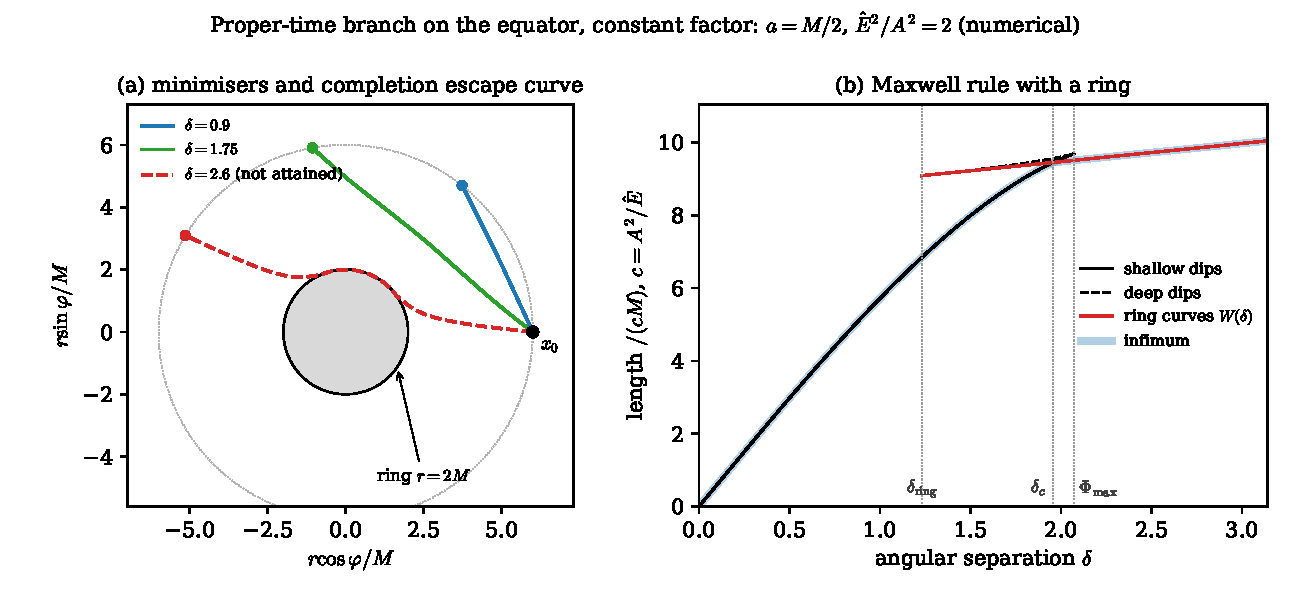
\includegraphics[width=\textwidth]{../figures/fig7_tau_ring.pdf}
\caption{Proper-time branch on the equator for a constant factor, $a=M/2$, $\Ehat^2/A^2=2$,
$r_0=r_f=6M$ (numerical, not certified). (a) Minimizers in the equatorial plane, drawn in the coordinates $(r\cos\varphi,r\sin\varphi)$ (not an isometric embedding of $h_\tau$; the ring has coordinate radius $2M$ and length $2\pi\rho_h$): shallow dips for
$\delta<\delta_c$, and for $\delta>\delta_c$ the tangent--arc--tangent curve of the completion, which no
rail attains. (b) Lengths against the separation: shallow and deep dips, the ring curves
$W(\delta)=\mathcal S(r_0)+\mathcal S(r_f)+\rho_h\delta$, and the infimum (Theorem~\ref{thm:tau-eq-maxwell});
here $\delta_{\rm ring}\approx1.232$, $\delta_c\approx1.956$, $\Phi_{\max}\approx2.072$.}
\label{fig:tau-eq-ring}
\end{figure}

\subsection{Time-dependent factor}
\begin{lemma}[kinematics at the ring]\label{lem:tau-eq-kin}
For $a>0$:
\begin{enumerate}
\item the largest radial speed in $K$ is $\sqrt{f\Delta}/(r\sqrt{N-|\beta|^2})$, with the positive limit
  $a\Ehat/(2M\sqrt{A^2+2\Ehat^2(1+2M^2/a^2)})$ at $r=2M$; the ring is reached in finite conformal time;
\item along circular rails the conformal time per radian is $T_\pm=(\sqrt{N\Delta}\mp2Ma/r)/f$, with
  $T_+(2M)=a+aA^2/(2\Ehat^2)+2M^2/a$ finite and $T_-\sim4aM/(r-2M)$;
\item waiting at radius $r$ costs $\omega$ per unit time, which vanishes at the ring;
\item the clock along the tangent geodesic to the ring is finite in the prograde sense and
  diverges logarithmically in the retrograde sense.
\end{enumerate}
\end{lemma}

\begin{proof}
(1) In the variables $X=r\dot r/\sqrt{f\Delta}$, $Y=\sqrt\Delta\,\dot\varphi/f$ the constraint is
$-|\beta|Y+\sqrt N\sqrt{X^2+Y^2}\le1$; the maximum of $(1+|\beta|Y)^2/N-Y^2$ is $1/(N-|\beta|^2)$, and
$1-|\beta|^2=fg_{\varphi\varphi}/\Delta$. (2)--(3) are direct. (4) Along a curve with $\dd r/\dd\varphi=u$ the
prograde clock per radian is at most $T_+(r)+\sqrt N r^2u^2/(2\Delta^{3/2})$, bounded for bounded
$u$; in the retrograde sense it is at least $T_-\ge c/(r-2M)$, while $\dd\varphi/\dd r$ has a positive
limit at the ring.
\end{proof}

For a class $\Lambda$ define the escape price $B(\Lambda)$ as the limit, as $\epsilon\to0$, of the infimum of
the cost over relaxed curves of the class, of finite duration, that come within $\epsilon$ of $r=2M$.

\begin{theorem}[existence for finite variations]\label{thm:tau-eq-exist}
Let $A$ be as at the beginning of this section.
\begin{enumerate}
\item $B(\Lambda)\ge\mathcal B_{a_*}(|\Lambda|)$, and every curve of the class costs at least $\rho_h(a_*)|\Lambda|$.
\item If the infimum $m$ satisfies $m<\min_\Lambda B(\Lambda)$, a global minimizer exists and every minimizer
  is a rail curve.
\item In particular, with $d_\alpha$ the distance in the frozen completion for the factor $\alpha$ and
  $\Gamma=(A_{\max}/a_*)^2\sqrt{(\Ehat^2-a_*^2)/(\Ehat^2-A_{\max}^2)}$,
  \[
    d_{a_*}\le m\le d_{A_{\max}}\le\Gamma\,d_{a_*},
  \]
  and $\Gamma d_{a_*}(x_0,x_f)<\mathcal B_{a_*}(\delta)$ implies the existence of a minimizer for every
  $A\in C^1$ with values in $[a_*,A_{\max}]$, with no condition on $A'$.
\end{enumerate}
\end{theorem}

\begin{proof}
(1) Lemma~\ref{lem:tau-eq-relax}(1) and Proposition~\ref{prop:tau-eq-price}. (2) Choose a bounded-cost minimizing sequence. The angular lower bound in (1) leaves only finitely
many lifts; pass to a subsequence of fixed lift $\Lambda$. If its minimum radius approached $2M$, the
definition of $B(\Lambda)$ would give $m\ge B(\Lambda)$, a contradiction; thus it stays in
$r\ge2M+\epsilon$. The bound $C\ge L_{a_*}$ and $\dd s\ge|\dd R_{a_*}|$ give an outer radial barrier. On this
shell the rate is at least $a_*^2f(2M+\epsilon)/(2\Ehat)$, so durations and coordinate velocities are
bounded. Compactness, Lemma~\ref{lem:tau-eq-relax}(2) and Proposition~\ref{prop:tau-eq-rail} give
an attained rail minimizer. (3) Near-minimizing frozen rails for $A_{\max}$ are admissible for $A$ with no larger cost
(Lemma~\ref{lem:tau-eq-relax}(4)); since $|\Lambda_j|\ge\delta$ and $\mathcal B_{a_*}$ is non-decreasing, the
criterion excludes every escape. The ratio of the frozen densities,
$(A_{\max}^2/a_*^2)\sqrt{(\Ehat^2-a_*^2f)/(\Ehat^2-A_{\max}^2f)}$, is non-decreasing in $f\le1$.
\end{proof}

\begin{theorem}[asymmetry of the escape price]\label{thm:tau-eq-asym}
Let $a>0$, $A\ge A_0$ on $[\eta_0,\infty)$ and $A\equiv A_0$ on $[\eta_0,\eta_0+T_*]$. For a fixed lifted
class with $\Lambda\ge\delta_{\rm ring}(A_0)$, suppose that $T_*$ exceeds the limiting clock duration of its
prograde tangent--arc--tangent curve, and that $A\ge A_0+\kappa$ on $[\eta_2,\infty)$ for some $\eta_2$ and
$\kappa>0$. Then $B(+\Lambda)=W_{A_0}(\Lambda)<B(-\Lambda)$. This compares the two lifted classes, not the
prices minimized over all lifts of a physical target.
\end{theorem}

\begin{proof}
Both prices are at least $W_{A_0}$ by Theorem~\ref{thm:tau-eq-exist}(1). Interior approximations of
the prograde ring curve have clocks converging to its limiting duration
(Lemma~\ref{lem:tau-eq-kin}(4)), which is less than $T_*$, so they run inside the window. For the
retrograde class put $T^{\rm base}=(\sqrt\Delta+2Ma/r)/f\le T_-$ and $T_n=\min(T^{\rm base},n)$; every relaxed
curve satisfies $\dd\eta\ge T_n(r)(\dd\varphi)^-\ge-T_n\,\dd\varphi$. Use the frozen radial coordinate $R=R_{A_0}(r)$
and parametrize the curves by length on a common interval. For each fixed $n$ the form
$\theta_n=-T_n(R)\,\dd\varphi$ is constant in $R$ near the ring and Lipschitz on the compact set in question;
for uniformly convergent curves of bounded length, Stokes' formula on the straight homotopy in
$(R,\varphi)$ bounds the difference of its integrals by
$C_n\|\gamma_k-w_-\|_\infty(\operatorname{len}\gamma_k+\operatorname{len}w_-)+o(1)$, so the integrals converge for fixed
$n$. Only afterwards let $n\to\infty$: on the retrograde ring curve $w_-$ they diverge, since
$T^{\rm base}\asymp(r-2M)^{-1}$ and $|\dd\varphi/\dd r|$ has a positive limit on a retrograde tangent. If
$B(-\Lambda)=W_{A_0}$, take curves of costs $C_k\to W_{A_0}$ and split them at $\min(T_k,\eta_2)$. The calibration gives
$L_{A_0}(\gamma_k)\ge W_{A_0}-o(1)$, and the late overprice, with factor $((A_0+\kappa)/A_0)^2-1>0$, forces the
frozen length of the late parts to zero; they end at the target, so the near contact with the ring
belongs to the early parts. These have end points converging to $x_f$ and lengths tending to
$W_{A_0}$; a subsequence parametrized by length converges to the unique equality case $w_-$, while
their clocks stay below $\eta_2-\eta_0$, contradicting the divergence above.
\end{proof}

Where the value function $V(\eta,x)$, the infimum of the cost from $(\eta,x)$ to $x_f$, is
differentiable off the target, it satisfies the Hamilton--Jacobi--Bellman equation
\begin{equation}
  V_\eta+\omega-\sigma_K(\omega\beta-D_xV)=0,\qquad
  \sigma_K(\xi)=\frac{\sqrt{(\xi\cdot\beta^\sharp)^2+(N-|\beta|^2)|\xi|^2}-\xi\cdot\beta^\sharp}{N-|\beta|^2},
  \label{eq:tau-eq-hjb}
\end{equation}
with $V(\eta,x_f)=0$, or equivalently $\gopt^{-1}(\theta+\dd V,\theta+\dd V)=0$ with
$\omega+V_\eta\ge0$. With $\mathcal H_\alpha(x,p)=-\omega_\alpha+\sigma_{K_\alpha}(p+\omega_\alpha\beta)$, regular
characteristics satisfy $\dot X=\partial_p\mathcal H_{A(\eta)}$, $\dot P=-\partial_x\mathcal H_{A(\eta)}$, $P=-D_xV$, and
$p_\eta=-V_\eta$. More generally, let $U$ be locally Lipschitz on a domain containing all competitors
under consideration, and suppose that every covector $\xi=(\xi_\eta,\xi_x)$ of its Clarke
differential~\cite[section~4.7]{Vinter2000} satisfies $|\xi_x+\xi_\eta\beta|\le\sqrt N(\omega+\xi_\eta)$ and $\omega+\xi_\eta\ge0$. If $U(T,x_f)\le0$ for every
admissible arrival clock (and every target lift, when using the cover), then
$C(\gamma)\ge U(\eta_0,x_0)-U(T,x_f)\ge U(\eta_0,x_0)$. A candidate $\gamma_*$ is a global minimizer if, in
addition, $(U\circ\gamma_*)'+\theta(\gamma_*')=0$ almost everywhere and $U(T_*,x_f)=0$.

\begin{theorem}[global selection for finite variations]\label{thm:tau-eq-select}
Let $A\equiv A_*$ on $[\eta_*,\infty)$, with $q_*=\Ehat^2/A_*^2\ge3/2$, and let $d_*=d_{A_*}(\cdot,x_f)$.
\begin{enumerate}
\item \emph{Change after arrival.} If the frozen problem for $A_0$ has a unique minimizer $\gamma_0$,
  arriving at $T_0$, and $A\equiv A_0$ on $[\eta_0,T_0]$, $A\ge A_0$ afterwards, then $\gamma_0$ is the unique
  global minimizer.
\item \emph{Short initial window.} Let $A$ be arbitrary in $[a_*,A_{\max}]$ on $[\eta_0,\eta_*]$, of
  length $\tau$. Assume that $d_*$ is $C^2$ on a neighborhood of a closed coordinate ball
  $\bar B_R(x_0)\subset\{r>2M\}$, disjoint from every lift of the target, with unique and attained
  physical frozen tails; that on
  $\mathcal D=\{x\in\bar B_R,\ |p+Dd_*(x)|\le s\}$ the quantity $|p+\omega_\alpha\beta|$ is bounded below by
  $\chi>0$ for $\alpha\in[a_*,A_{\max}]$; and let $V_{\rm loc}$ bound the coordinate speeds of $K_\alpha$ on
  $\bar B_R$, $M_x,M_p,L$ bound the two components of $(\partial_p\mathcal H_\alpha,-\partial_x\mathcal H_\alpha)$ and
  its derivative on $\mathcal D$, and $S=\sup|D^2d_*|$, $B_0=1+S$ (here, exceptionally, Euclidean norms
  in $(r,\varphi)$ and in $(x,p)$).
  If
  \[
    \tau V_{\rm loc}<R/4,\qquad \tau(M_p+SM_x)<s/2,\qquad B_0(e^{L\tau}-1)<1/2,
  \]
  then the global minimizer exists and is unique; it crosses $\eta_*$ and its tail is the frozen
  minimizer. No assumption is made on $A'$.
\end{enumerate}
\end{theorem}

\begin{proof}
(1) Every competitor is admissible for $A_0$ with a cost not larger
(Lemma~\ref{lem:tau-eq-relax}(4)), hence costs at least the frozen minimum, which $\gamma_0$ attains
inside the window; equality forces a frozen relaxed minimizer, i.e.\ $\gamma_0$.

(2) Before any first exit from $\bar B_R$, every relaxed curve from $x_0$ has displacement at most
$\tau V_{\rm loc}<R/4$. Thus no first exit from $B_{R/4}$ is possible before $\eta_*$, and no target lift
is reachable by that clock. Integrate the characteristics backwards from $X(\eta_*,z)=z$,
$P(\eta_*,z)=-Dd_*(z)$, for $z\in\Omega:=\bar B_{R/2}(x_0)$. Up to a possible first exit from $\mathcal D$,
one has $\partial_p\mathcal H\in\partial K$ and hence
\[
  |X-z|\le\tau V_{\rm loc}<R/4,\qquad |P+Dd_*(X)|\le\tau(M_p+SM_x)<s/2 .
\]
These bounds keep $X$ in $B_{3R/4}$ and exclude a first exit from the tube.

The variational matrix $Y=D_z(X,P)$ starts at $(I,-D^2d_*)^{\mathsf T}$, with norm at most $B_0$. Since
the canonical flow and its state derivative depend on $A$, not on $A'$, Gr\"onwall gives
$|D_zX-I|\le k:=B_0(e^{L\tau}-1)<1/2$. Convexity of $\Omega$ yields $|X(\eta,z)-X(\eta,w)|\ge(1-k)|z-w|$.
Writing $X=z+e_\eta(z)$, the map $z\mapsto x-e_\eta(z)$ is a contraction of $\Omega$ into itself for every
$x\in B_{R/4}$, because $\|e_\eta\|_\infty<R/4$. Hence the projected field covers $B_{R/4}$ injectively at
every clock.

Define on the covered region $V(\eta,X(\eta,z))=d_*(z)+\int_\eta^{\eta_*}\omega(1-\beta(\dot X))\,\dd s$.
Variation of the canonical action, with terminal covector $-Dd_*$, gives $D_xV=-P$ and $V_\eta=\mathcal H$.
For $v\in K$,
\[
  c_A(v)+V_\eta+D_xV\cdot v=\sigma_K(P+\omega\beta)-(P+\omega\beta)\cdot v\ge0,
\]
with equality at a unique velocity since $\chi>0$. For an arbitrary competitor with junction
$y=x(\eta_*)$, the prefix costs at least $V(\eta_0,x_0)-d_*(y)$ and the tail at least $d_*(y)$,
including non-attained tails approximated by escape curves. The characteristic through $x_0$
followed by its attained frozen tail has total cost $V(\eta_0,x_0)$. In the equality case the
prefix solves the unique spatially $C^1$ field and the tail is the unique frozen one.
\end{proof}

No smallness of the amplitude or of $A'$ is required in~(2); the duration bound depends on the
frozen field and on the allowed interval $[a_*,A_{\max}]$. For example, a pulse
$A=A_*-b\sin^2(\pi(\eta-\eta_0)/\tau)$ of fixed allowed depth $b$ has $\|A'\|_\infty=\pi b/\tau\to\infty$.

\begin{corollary}[perturbative equatorial selection]\label{cor:tau-eq-P}
Let $0<A_0<\Ehat$, $q_0=\Ehat^2/A_0^2$, and $0<\delta<\pi$. Suppose that the frozen equatorial problem has a unique interior
global minimizer $\gamma_0$, with non-degenerate free-arrival shooting map and cost
$C_0<\mathcal B_{A_0}(\delta)$. There exists $\varrho>0$ such that $\|A-A_0\|_{C^1_b([\eta_0,\infty))}<\varrho$ gives a
unique global equatorial minimizer, with shooting data close to those of $\gamma_0$. For
$A_\epsilon=A_0+\epsilon\alpha$, $\alpha\in C^1_b$,
\[
  m_\epsilon=C_0+\epsilon\int_{\eta_0}^{T_0}\frac{A_0f(N_0+1)}{\Ehat}\bigl(1-\beta(\dot x_0)\bigr)\alpha(\eta)\,\dd\eta+o(\epsilon).
\]
The frozen hypotheses hold for $q_0\ge3/2$ and $0<\delta<\delta_c$, including unequal radii and the
tangent separation.
\end{corollary}

\begin{proof}
Choose $a_*<A_0$ close enough that $C_0<\mathcal B_{a_*}(\delta)$; this is possible because the ratio of
the frozen densities tends to one uniformly. Theorem~\ref{thm:tau-eq-exist}, with a slowed frozen
competitor, supplies minimizers in a common shell and a common finite clock window, and
compactness brings every minimizer to $\gamma_0$ as $A\to A_0$. The clock equation gives
$p_\eta=O(\|A'\|_\infty)$, so $\omega-p_\eta$ stays positive on the shell; the normal shooting data are therefore
compact and approach the reference data. Non-degeneracy and the implicit-function argument of
Theorem~\ref{thm:tau-P}, restricted to equatorial competitors, identify a unique zero containing
every global minimizer. At the frozen reference $p_\eta=0$, and differentiating the Hamiltonian action
gives the first variation. The strict frozen barrier follows from the corner shortcut below
$\delta_{\rm ring}$ and from the Maxwell rule above it.
\end{proof}

As in Theorem~\ref{thm:tau-P}, global $C^1$ closeness may be replaced by closeness on a common
competitive window, provided global bounds and a uniform strict escape margin already supply that
window.

\begin{remark}[an example]\label{rmk:tau-eq-example}
Let $M=1$, $a=1/2$, $\Ehat=\sqrt2$, $r_0=6$, $\eta_0=0$, a target at radius $6$ with $\varphi_f=\pm1/50$, so
$\delta=1/50$, and $A=1-\frac12\sin^2(\pi\eta/\tau)$ on $[0,\tau]$, $A=1$ afterwards. Write $m_\pm$ for the two
targets. The following are proved.
\begin{itemize}
\item \emph{Early arrival is impossible for $\tau\le7/50$.} Since $|\dot r|^2\le\Delta^2/(r^2g_{\varphi\varphi})<1$
  and the largest angular speed is that of the circle, $T_+\ge4394/625$ on $r\ge293/50$, so no curve
  sweeps $1/50$ by then.
\item \emph{All minimizers arrive early for $1/5\le\tau\le1$.} For $1/5\le\tau\le2/5$, every curve with
  $T\ge\tau$ costs at least $(5985/23296)\tau>\tau/4$, while the prograde and retrograde circles at $r=6$,
  run with the actual clock, arrive before $\tau$ and cost less than $\tau/4$. For $2/5\le\tau\le1$, the
  respective bounds are $57\tau/256\ge57/640$ and $\sqrt{291}/200$, with strict gap
  $57/640-\sqrt{291}/200>0$. Uniqueness holds for every $\tau$ (Theorem~\ref{thm:tau-eq-unique}).
\item \emph{Continuity and asymmetry.} $m_\pm$ is continuous in $\tau>0$; $m_+<m_-$ for small $\tau$ and
  $m_-<m_+$ for large $\tau$.
\end{itemize}
For $\tau\le2/5$, the radial speed bound gives $r\ge28/5$ on every crossing prefix; hence $f\ge9/14$,
$|\beta|<1/25$ and $c_A\ge(315/728)A^2$, while $\int_0^\tau A^2\,\dd\eta=19\tau/32$. The two circles last less
than $9/50$ and $93/500$, and their cost rates divided by $A^2$ are below $1/2$ and $10/21$. With
$F(\nu)=\int_0^\nu(1-\frac12\sin^2\pi u)^2\,\dd u$ one has $F(1)=19/32$ and $F(1)-F(1-h)>h-10h^3/3$; taking
$h=1/10$ and $7/100$ gives $F(9/10)<1/2$ and $F(93/100)<21/40$, hence both circle costs are below
$\tau/4$ for $\tau\ge1/5$. For $\tau\le1$, instead, $r\ge5$, $f\ge3/5$ and $|\beta|<1/15$ give $c_A\ge(3/8)A^2$;
the frozen circle length bounds both actual circle costs by $\sqrt{291}/200$, and both durations are
below $2/5$.

For existence and uniform compactness, the circle gives $m\le U:=\sqrt{291}/200$, whereas
$\mathcal B_{1/2}(1/50)\ge2R_{1/2}(6)\ge4/\sqrt{97}>U$, by $r(r-2)/\Delta\ge32/97$ on $[4,6]$. A level
$U<\bar C<\mathcal B_{1/2}$ thus gives a common shell and clock duration $H$ for all competitive curves,
independently of $\tau$. As $\tau\to\tau_0>0$ the profiles converge in $C^1([0,H])$; compactness gives
lower semicontinuity of the value, and lifting a fixed minimizing spatial curve with the nearby
clock gives upper semicontinuity, preserving the target exactly. Hence $m_\pm$ is continuous.

The frozen reference at $A=1$ is unique and non-degenerate: $\delta_{\rm ring}\ge128/(291\sqrt{194})$, which
exceeds $1/50$.
In the example the frozen launch has non-zero radial momentum and $\beta$ has only an angular
component, so the canonical field stays uniformly regular for $\alpha\in[1/2,1]$ in a tube around the
frozen geodesic. For short windows, rescaling $u=\eta/\tau$ and using this field gives
$m_\pm=C_0-\tau\int_0^1\mathcal H_{\alpha(u)}(x_0,p_\pm)\,\dd u+O(\tau^2)$, where $\alpha(u)=1-\frac12\sin^2\pi u$. The
reflected frozen costates have the same radial component and norm, $|p_\pm|^2=N_1\omega_1^2$, and
$p_\varphi=\pm L$. Put $B=p\cdot\beta^\sharp$ and $h=\mathcal H_\alpha$. For $\alpha<1$, $N_\alpha\omega_\alpha^2<N_1\omega_1^2$, the
selected root is positive and
\[
  (N-|\beta|^2)h^2+2(N\omega+B)h+N\omega^2-|p|^2=0,\qquad
  \partial_Bh=-\frac{h}{(N-|\beta|^2)h+N\omega+B}<0,
\]
the denominator being positive on the selected root. Since $B_+<B_-$, $m_+<m_-$ for sufficiently
small $\tau$. For long windows, on the common competitive interval,
$A_\tau(\eta)=1-\pi^2\eta^2/(2\tau^2)+O(\tau^{-4})$ in $C^1$, and the local-window form of
Corollary~\ref{cor:tau-eq-P} gives
\[
  m_\pm=C_0-\frac{\pi^2}{2\tau^2}I_\pm+o(\tau^{-2}),\qquad I_\pm=\int_0^{C_0}(N+1)\,\eta_\pm(\ell)^2\,\dd\ell,
\]
with $\ell$ the frozen proper length along the reflected geodesics and $\eta_\pm(0)=0$. Their clocks
satisfy $\dd\eta_\pm/\dd\ell=1/\omega\pm\beta_\varphi\varphi_+'(\ell)$, so $\eta_->\eta_+$ for $\ell>0$, $I_->I_+$ and $m_-<m_+$
for sufficiently large $\tau$. At least one equality of the two target costs follows by continuity;
this is not a Maxwell tie in one problem.

Floating-point diagnostics, not certified: multi-start free-arrival shooting returned one accepted
solution at each of twelve sampled values of $\tau\in[0.12,0.20]$ in each sense. The reported arrival
times lie on opposite sides of $T=\tau$ at $\tau=0.160,0.165$ (prograde) and at $\tau=0.170,0.175$
(retrograde). At every sampled parameter the reported prograde candidate has lower cost than the
retrograde candidate. The proof of Theorem~\ref{thm:tau-eq-unique} shows that an exact zero of
the shooting map in the rectangle $Q_s$ of that proof is unique and coincides with the global minimizer, by existence and
localization of all minimizers. The numerical shooting outputs and their apparent brackets
remain uncertified diagnostics; no rigorous error bound is assigned to them here. A unique
transversal sector change, with rational enclosures for the global minimizer, is proved
analytically in Theorem~\ref{thm:tau-eq-sector}.
\end{remark}

\subsection{Global uniqueness in the example}
We keep the data of Remark~\ref{rmk:tau-eq-example}: $M=1$, $a=1/2$, $\Ehat=\sqrt2$, $x_0=(6,0)$, the
target $x_f=(6,s/50)$ with $s=\pm1$, and $A_\tau(\eta)=1-\frac12\sin^2(\pi\eta/\tau)$ on $[0,\tau]$, $A_\tau=1$
afterwards; $A_\tau$ is of class $C^1$ and takes values in $[1/2,1]$. On the equator
$\Delta=r^2-2r+\frac14$, $h_r=r^2/(f\Delta)$, $h_\varphi=\Delta/f^2$, $\beta_\varphi=-1/(r-2)$ and
$|\beta|^2_{h_0}=1/(r^2\Delta)$. Write $p=(p_r,J)$ for the costate, $J=p_\varphi$, $j=|J|$, $g=A^2/(\sqrt2r)$,
so that the angular component of $p+\omega\beta$ is $\xi=J-g$, and put
\[
  d=N-|\beta|^2_{h_0},\quad a_H=\frac1{dh_r},\quad b_H=\frac N{d^2h_\varphi},\quad k_H=\frac{\beta_\varphi}{dh_\varphi},\quad
  S=\sqrt{a_Hp_r^2+b_H\xi^2}.
\]
The support function in~\eqref{eq:tau-eq-hjb} gives the Hamiltonian
$\mathcal H=-\omega+S-k_H\xi$, with $\dot r=a_Hp_r/S$ and $\dot\varphi=b_H\xi/S-k_H$. All derivatives in $r$ are
taken at fixed $(A,p_r,J)$. We use the shell $\mathcal S=\{23/4\le r\le25/4\}$; on it $h_r$ and $|\beta|^2_{h_0}$
decrease, $h_\varphi$, $f$ and $N$ increase (with $\Delta<(r-1)^2$,
$(\log h_r)'=3/r-1/(r-2)-2(r-1)/\Delta<(6-4r)/(r(r-1)(r-2))<0$ and
$(\log h_\varphi)'=2(r-1)/\Delta-4/(r(r-2))>2(r^2-4r+2)/(r(r-1)(r-2))>0$ for $r>2+\sqrt2$), and $184/169\le N\le50/33$, $h_r\ge15625/7293$,
$184621/3600\le h_\varphi\le268125/4624$, $|\beta|^2_{h_0}\le256/(23^2\cdot349)$. At $r=6$ write
$c_r(A)=\omega\sqrt{Nh_r}$ and $c_\varphi(A)=\omega\sqrt{Nh_\varphi}$; they increase with $A$, with
$c_r^2\in[36/1067,72/97]$ and $c_\varphi^2\in[291/352,291/16]$ on $[1/2,1]$, and $c_r/c_\varphi=\kappa_6$ with
$\kappa_6^2=3456/84681$, $1/5<\kappa_6<203/1000$.

\begin{proposition}[localization]\label{prop:tau-eq-loc}
Let $\tau>0$ and $s=\pm1$. Every relaxed curve from $x_0$ to any lift of the target with cost at most
$7/80$ satisfies $23/4<r<25/4$, $\operatorname{Var}\varphi<7/64$ and $T<35/44$; since $m_s\le\sqrt{291}/200<7/80$,
every global minimizer ends at the principal lift $\varphi_f=s/50$. Every global minimizer is a normal
rail extremal, with $\varphi$ monotone, and
\[
  \begin{array}{l}
  \tfrac{3}{25}<T<\tfrac{21}{100},\quad |r-6|<\tfrac1{50},\quad |p_r|<\tfrac{63}{2000},\quad
  \operatorname{sign}J=s,\\[2pt]
  j>\tfrac89,\quad |p+\omega\beta|_{h_0^{-1}}>\tfrac1{10},\quad |\psi(T)-s\tfrac\pi2|<\tfrac15 .
  \end{array}
\]
Here the representative of the terminal heading is chosen around $s\pi/2$ modulo $2\pi$.
\end{proposition}

\begin{proof}[Structure of the proof]
Leaving the shell and returning costs more than $7/80$, by the radial coefficient of the frozen length at
$A=1/2$, while the circle $r=6$ run with the actual clock costs less; inside the shell the angular coefficient
bounds the angle, and $\omega$ bounds the duration. A minimizer is a normal extremal; since its radius
returns to $6$, the radial costate vanishes somewhere, and a force bound on the shell keeps it small. The
terminal ellipse given by transversality then bounds $j$ from below, so the angular speed is bounded below
and $\varphi$ is monotone; this bounds $T$, and repeating the steps sharpens the bounds on $p_r$, $j$, $r$ and
the terminal heading. The constants are in
section~\ref{S-sec:supp-tk-example} of the supplementary material.
\end{proof}

\begin{proposition}[late sector]\label{prop:tau-eq-late}
For $\tau\le\tau_{\rm no}:=1425548384/9363983275\approx0.15224$ no relaxed curve reaches a lift of the
target by the clock $\tau$; every minimizer crosses $\eta=\tau$. For $\tau\ge1/5$ every minimizer arrives
before $\tau$.
\end{proposition}

\begin{proof}
For $\tau\le1/5$, $|\dot r|<1$ keeps $r\ge29/5$ up to the clock $\tau$, where the largest angular speed
is the prograde circular one, $|\dot\varphi|\le1/D_+$ with $D_+=\sqrt N\sqrt\Delta/f-1/(r-2)$. On $r\ge29/5$,
$\sqrt\Delta/f>36/5$, $f\ge19/29$ and $\sqrt N\ge1+(19/116)A^2$, so $D_+>b_*+k_*A^2$ with $b_*=659/95$,
$k_*=171/145$. The function $z\mapsto1/(b_*+k_*z)$ is convex, hence below its chord on $[1/4,1]$, and
$\int_0^1(1-\frac12\sin^2\pi u)^2\,\dd u=19/32$; therefore
$\operatorname{Var}\varphi<\tau K\le1/50$ with $K=374559331/2851096768=1/(50\tau_{\rm no})$. The second statement
is Remark~\ref{rmk:tau-eq-example} for $1/5\le\tau\le1$, and Proposition~\ref{prop:tau-eq-loc}
($T<21/100$) for $\tau\ge21/100$.
\end{proof}

\begin{lemma}[a triangular criterion]\label{lem:tau-eq-triang}
Let $Q=[T_1,T_2]\times[-\theta_0,\theta_0]$ and $F=(F_1,F_2)\in C^1(Q,\mathbb R^2)$. Suppose that
$\partial_\theta F_2>0$ on $Q$, that $F_2(T,-\theta_0)<0<F_2(T,\theta_0)$ for every $T$, and that $\det DF>0$ on
$\{F_2=0\}$. Then $F$ has at most one zero in $Q$.
\end{lemma}

\begin{proof}
For every $T$ there is a unique $\theta^*(T)\in(-\theta_0,\theta_0)$ with $F_2(T,\theta^*(T))=0$, and $\theta^*$ is
$C^1$ with $\theta^{*\prime}=-\partial_TF_2/\partial_\theta F_2$. The zeros of $F$ are the points $(T,\theta^*(T))$ at which
$\Gamma(T)=F_1(T,\theta^*(T))$ vanishes, and $\Gamma'=\det DF/\partial_\theta F_2>0$.
\end{proof}

\begin{theorem}[global uniqueness in the example]\label{thm:tau-eq-unique}
For every $\tau>0$ and each sense $s=\pm1$, the global minimizer of the example is unique, as a
curve parametrized by the clock up to its arrival.
\end{theorem}

\begin{proof}[Structure of the proof]
For $(T,\theta)$ in a rectangle of arrival clocks and terminal headings, integrate the canonical system
backwards from the target and let $F_s(T,\theta)=(-s\varphi(0),s(r(0)-6))$; by Proposition~\ref{prop:tau-eq-loc}
every minimizer is a zero. The whole family stays regular in the shell, and $F_2$ has opposite signs on the two
sides $\theta=\mp1/5$. On the returning shots $F_2=0$ the radial costate is small and has zero mean
against a weight of bounded ratio. Explicit bounds on the coefficients of the variational system then give
$\partial_\theta F_2>0$ on the rectangle and $\det DF_s>0$ on $F_2=0$, and Lemma~\ref{lem:tau-eq-triang} allows at most one zero. The constants are in
section~\ref{S-sec:supp-tk-example} of the supplementary material.
\end{proof}

The uniqueness argument uses, in addition to the existence and localization premises,
only that $A\in C^1$ takes values in $[1/2,1]$ and that
$T|({\log c_\varphi(A(T))})'|\le46/7$ on $[3/25,21/100]$;
no bound on $A'$ along the trip is needed. The constants used in the proof are
obtained by rational comparisons. Floating-point checks, not certified, give
$D_{2\theta}/T\ge0.52$ on the sampled shots in $Q_s$, and
$\Gamma'\ge0.10$ on the separately sampled radial-return curves $F_2=0$.
These sampled values are diagnostics, not uniform bounds used in the proof.

\begin{corollary}[the sector change]\label{cor:tau-eq-sector}
The arrival time $T_s(\tau)$ of the minimizer is continuous in $\tau>0$; $T_s(\tau)>\tau$ for
$\tau\le\tau_{\rm no}$ and $T_s(\tau)<\tau$ for $\tau\ge1/5$. In particular the minimizer changes sector at
least once, at a clock $\tau$ with $T_s(\tau)=\tau$ in $(\tau_{\rm no},1/5)$.
\end{corollary}

\begin{proof}
Fix $\tau_0>0$ and the unique zero $(T_0,\theta_0)$ of the shooting map.
Write $A_\tau(\eta)=\alpha(\eta/\tau)$, where
$\alpha(\nu)=1-\frac12\sin^2(\pi \nu)$ for $0\le \nu\le1$ and $\alpha(\nu)=1$ for $\nu\ge1$.
Since $\alpha'(1)=0$, the profile is jointly $C^1$ in $(\eta,\tau)$ for $\tau>0$,
with $\partial_\tau A_\tau=-(\eta/\tau^2)\alpha'(\eta/\tau)$.
The regular canonical flow and its terminal data therefore make $F_s$
jointly $C^1$ in $(T,\theta,\tau)$ near this zero.
The zero is in the interior of $Q_s$ by Proposition~\ref{prop:tau-eq-loc},
and $\det D_{(T,\theta)}F_s>0$ by the proof of Theorem~\ref{thm:tau-eq-unique}.
The implicit-function theorem gives a local $C^1$ branch of zeros.
For each nearby $\tau$, a global minimizer exists, lies in $Q_s$ and is a zero;
the same proof shows that there is at most one zero in $Q_s$.
Thus the local branch is precisely the branch of global minimizers.
In particular $T_s$ is continuous at $\tau_0$ (indeed $C^1$).
The signs follow from Proposition~\ref{prop:tau-eq-late}, and the intermediate-value
theorem gives a sector change in $(\tau_{\rm no},1/5)$.
\end{proof}

\begin{theorem}[a single transversal sector change]\label{thm:tau-eq-sector}
For each sense $s$, $T_s\in C^1((0,\infty))$ and there is exactly one $\tau_s^*>0$ with $T_s(\tau_s^*)=\tau_s^*$:
the minimizer crosses $\eta=\tau$ for $\tau<\tau_s^*$ and arrives before $\tau$ for $\tau>\tau_s^*$. The change is
transversal, $T_s'(\tau_s^*)-1<-49/71$, and
\[
  \tfrac{159}{1000}<\tau_+^*<\tfrac{161}{1000}<\tfrac{169}{1000}<\tau_-^*<\tfrac{172}{1000}.
\]
\end{theorem}

\begin{proof}[Structure of the proof]
Corollary~\ref{cor:tau-eq-sector} gives $T_s\in C^1$ and at least one zero of $\Theta_s=T_s-\tau$ in
$(\tau_{\rm no},1/5)$. At a zero $A(T)=1$, which sharpens all bounds. Along the diagonal $T=\tau$ a
dilation of the clock leaves the profile and the terminal datum unchanged, and gives the derivative
$\Gamma_T+\Gamma_\tau$ of the angular miss on the returning shots, bounded below, while $\Gamma_T$ is bounded above;
hence $\Theta_s'<-49/71$ at every zero, which is therefore unique and transversal. At the zero
$1/50=\tau\int_0^1s\dot\varphi\,\dd \nu$; chord and Jensen bounds for the mean angular speed, concave in $A^2$,
enclose $\tau_\pm^*$. The constants are in
section~\ref{S-sec:supp-tk-example} of the supplementary material.
\end{proof}

The proof uses the self-similar form $A_\tau=\alpha(\eta/\tau)$ with $\alpha(1)=1$, $\alpha'(1)=0$, and the mean
$\int_0^1\alpha^2=19/32$; it is not claimed for other families of profiles. Between $\tau_+^*$ and $\tau_-^*$ the
prograde minimizer already arrives early while the retrograde one still crosses the pulse; this is
not a statement about the order of the two costs. Floating-point root-finding (not certified)
gives $\tau_+^*\approx0.160195$ and $\tau_-^*\approx0.170226$, with $T_s'-1\approx-1.10$ and $-1.09$, consistent with the
theorem.

Not proved here: global uniqueness for general time-dependent profiles, the regime
$1<q<3/2$, and the comparison with three-dimensional competitors, for which
the clock of the paths near the poles enters the history of $A$.

% ======================================================================
\section{The proper-time branch of ingoing Vaidya}
\label{sec:vaidya-tau}
% ======================================================================
For ingoing Vaidya, $g=-f\,\dd v^2+2\,\dd v\,\dd r+r^2\dd\Omega^2$ with $f=1-2m(v)/r$, the mass
enters the seed itself rather than a conformal factor, and the Kodama selector $\partial_v$ is
the rail selector. Let $\Ehat>1$, let $m\in C^1$ be positive, write $s=\dd r/\dd v$,
$\zeta=\dd\Omega/\dd v$ and $w=\Ehat^2-f$, and work on $r>2m(v)$. For constant mass $m_0$ the
static change $v=t+r_*(r)$, $r_*'=1/f$, gives $\dd\tau=f\,\dd t/\Ehat$: the proper-time problem
is that of section~\ref{sec:tau} with $A=1$ and $M=m_0$, and we write $R(r)$ for the function
of proposition~\ref{prop:completion} with these values. Explicitly,
\[
 R(r)=\int_{2m_0}^{r}\frac{\dd s}{\sqrt{\Ehat^2-1+2m_0/s}}.
\]

\begin{lemma}[rail, cost and velocity body]\label{lem:vaidya-rail}
Along a rail curve $\dd\tau/\dd v=(f-s)/\Ehat$ and $r^2|\zeta|^2=w-(s+w)^2/\Ehat^2$. The
relaxed velocity body
\[
  K(v,r)=\{(s,\zeta):\ (s+w)^2/\Ehat^2+r^2|\zeta|^2\le w\}
\]
is a strictly convex ellipsoid whose boundary is the rail; it contains the origin in its
interior exactly when $0<f<\Ehat^2$, and on it $f-s\ge\Ehat(\Ehat-\sqrt w)>0$. For every
relaxed curve with radial end points $r_0$, $r_f$, the convexified cost is
\[
  \int\frac{f(v,r(v))}{\Ehat}\,\dd v-\frac{r_f-r_0}{\Ehat},
\]
a potential $\omega=f/\Ehat$ with $\partial_r\omega=2m/(\Ehat r^2)>0$, plus a boundary term. Every
radial passage, inward or outward, costs at least $|\dd r|/\sqrt{\Ehat^2-f}$.
\end{lemma}

\begin{proof}
The rail condition gives $\Ehat=f\dot v-\dot r$, and the normalization of $u$ gives the
ellipsoid; the cost identity is $\int(f-s)/\Ehat\,\dd v$ integrated by parts. The radial cost
per unit radius, $(f-s)/(\Ehat|s|)$, is monotone in $|s|$ in both directions and equals
$1/\sqrt w$ at the extreme speeds $s=-w\pm\Ehat\sqrt w$.
\end{proof}

The density $(f-s)/\Ehat$ is affine in $s$, so on $K$ it is the convexification of the rail
cost, not the physical proper time of a slower curve. As in lemma~\ref{lem:radial-red}, the
cost depends only on the radial profile, and the maximal angular speed
$\sqrt{w-(s+w)^2/\Ehat^2}/r$ of the rail with the same profile allows any angular length
not smaller than that of a relaxed competitor. Every relaxed curve therefore has a rail
curve of equal cost. In the following PMP formulas, $p_r,p_\Omega$ and $p_v$ are the costates for
the potential cost $\omega=f/\Ehat$, after removing the fixed boundary term $-\Delta r/\Ehat$; $p_v$ is
conjugate to the clock $v$. Set $S=(\Ehat^2p_r^2+|p_\Omega|^2/r^2)^{1/2}$; the support function of $K$
is $h=-wp_r+\sqrt w\,S$, positive for $p\neq0$ because $0\in\operatorname{int}K$, although the body is
translated. As in proposition~\ref{prop:tau-rail}, this excludes the abnormal case for a
relaxed minimizer attained with free final time inside the domain. For a normal extremal,
on the set where the spatial costate vanishes, the radial adjoint equation gives
$p_r'=\partial_r\omega>0$ almost everywhere; since an absolutely continuous function has zero
derivative almost everywhere on its zero set, that set has measure zero. At every other time
strict convexity makes the maximizing velocity a boundary point of $K$, so the minimizer is a
rail curve almost everywhere.

\begin{theorem}[existence with an arrival deadline]\label{thm:vaidya-exist}
Assume $m'\ge0$ on $[v_0,v_1]$, $m(v_0)>0$, $r_0>2m(v_0)$ and $r_f>2m(v_1)$. For every
angular separation, if the class of relaxed curves arriving at the target by $v_1$ is
non-empty, the minimum exists and is attained by a rail curve. Every non-trivial minimizer
is a rail curve almost everywhere.
\end{theorem}

\begin{proof}
For $x=r-2m(v)$ every relaxed curve has $\dot x\le x/(4m(v_0))-2m'$, since the outward speed is
at most $f/2$. Integrating backwards from the arrival,
$x(v)\ge(r_f-2m(v_1))\,e^{-(v_1-v_0)/(4m(v_0))}>0$, and $r\le r_0+(v_1-v_0)/2$. Speeds are bounded;
extending each curve by rest at $x_f$ after arrival, which is admissible and does not enter
the cost, Arzel\`a--Ascoli gives a uniform limit. In local coordinates along the curve (or
with $S^2$ embedded in $\mathbb R^3$), for every constant covector $a$ one has
$a\cdot y_n'\le\sigma_{K(v,y_n)}(a)$; integrating against non-negative test functions and using
the continuity of the support functions on the compact region, the limit satisfies
$y'\in K(v,y)$ almost everywhere. The cost of lemma~\ref{lem:vaidya-rail} contains no derivative
and passes to the limit. The radial reduction gives a rail minimizer. A minimizer with
$T<v_1$ is a normal extremal and a rail almost everywhere. If $T=v_1$, apply the fixed-time PMP.
In the normal case the same zero-set argument applies. In the abnormal case the spatial
adjoint system is homogeneous, so its non-trivial solution cannot vanish; strict convexity
again puts the maximizing velocity on $\partial K$ almost everywhere. Normality of such
minimizers is not claimed.
\end{proof}

With a finite deadline existence holds already at constant mass; it does not decide
attainment for unrestricted arrival time, where for constant mass and $\delta>\delta_c$ the
infimum is not attained.

\begin{theorem}[global selection near constant mass]\label{thm:vaidya-P}
Let $m_0>0$, $r_0,r_f>2m_0$, $0<\delta<\pi$, and let the arrival time be unrestricted.
Suppose that the frozen problem has a unique interior global minimizer $\gamma_0$ of cost
$C_0<R(r_0)+R(r_f)$ with non-degenerate planar shooting. There is $\varrho>0$ such that every
positive $m\in C^1$ with $\|m-m_0\|_{C^1_b([v_0,\infty))}<\varrho$ has a unique global proper-time
minimizer among all regular three-dimensional rail curves, the continuation of $\gamma_0$.
Its shooting data depend continuously on $m$, and
$|p_{v,{\rm in}}|\le C\|m'\|_{L^\infty([v_0,v_0+H])}$ for uniform $C,H$. For $m_\epsilon=m_0+\epsilon\beta$,
$\beta\in C^1_b$,
\[
  \tau_{\min,\epsilon}=C_0+\epsilon\int_{v_0}^{T_0}
  \Big[\frac{p_r}{r}-\frac{\Ehat^2+w}{\Ehat\,r\,w}\Big]_0\beta(v)\,\dd v+o(\epsilon),
\]
the bracket being evaluated along $\gamma_0$, where it is negative. No sign condition on $m'$ is
required.
\end{theorem}

\begin{proof}
Choose $C_0<C^*<R(r_0)+R(r_f)$; first $r_1>2m_0$ below $\gamma_0$ such that the radial cost of
descending to $r_1$ and returning, with weight $(\Ehat^2-1+2m_0/r)^{-1/2}$, exceeds $C^*$ with a
margin; then $m_+>m_0$ with $2m_+<r_1$ for which the same holds with $m_+$. For small $\varrho$,
$m\le m_+$ on the whole future, so by lemma~\ref{lem:vaidya-rail} every competitor of cost at most
$C^*$ stays in $r>r_1$, in a bounded shell, and has duration at most
$H=(\Ehat C^*+r_f-r_0)/f_{\min}$ with $f_{\min}=1-2m_+/r_1$. The frozen minimizer slowed by a factor
$\lambda<1$ has velocities in the interior of the frozen body $K_0$ with a uniform margin, since
$\lambda K_0+(1-\lambda)B_c\subset K_0$ when $K_0$ contains the ball $B_c$ of radius $c$ about the origin; it is admissible for small $\varrho$, with cost tending to
$(C_0+\Delta r/\Ehat)/\lambda-\Delta r/\Ehat$. Existence, convergence of all minimizers to $\gamma_0$,
normality and planarity follow as in theorems~\ref{thm:tau-exist} and~\ref{thm:tau-P}. Since $h$ is
positively homogeneous and $h\ge c|p|$, the condition $\mathcal H=p_v+h-\omega=0$ gives
$|p|\le C(\omega+|p_v|)$; the clock costate solves $p_v'=-m'\,\partial_m(h-\omega)$, $p_v(T)=0$, so Gr\"onwall
gives $\|p_v\|_\infty\le C_H\|m'\|$, after which $h=\omega-p_v$ bounds $|p|$ below. The shooting map
$(p_{r0},L,T_v)\mapsto(r(T_v)-r_f,\varphi(T_v)-\delta,p_v(T_v))$, with $p_v(v_0)$ fixed by $\mathcal H=0$,
involves $m$ and $m'$ only. At constant mass it is non-degenerate: the launch variables
$p_{r0}=(S_0/\Ehat)\cos\psi$, $L=S_0r_0\sin\psi$ give
$\det\partial(p_{r0},L)/\partial(\psi,p_{v,{\rm in}})=r_0S_0/(\Ehat b(\psi))>0$ with
$w_0=\Ehat^2-f(v_0,r_0)$, $b=\sqrt{w_0}-(w_0/\Ehat)\cos\psi$ and $S_0=(\omega_0-p_{v,{\rm in}})/b(\psi)$, positive near
the reference $p_{v,{\rm in}}=0$; the costates of the $v$ and $t$ conventions are related by
$p_t=p_v$, $L^{(t)}=L^{(v)}$, $p_r^{(t)}=p_r^{(v)}+p_v/f-1/\Ehat$, and the arrival clocks, measured from the
same launch, by $T_v=T_t+r_*(r(T_t))-r_*(r_0)$, with $\partial T_v/\partial T_t=1+(\dd r/\dd t)/f>0$.
Hence non-degeneracy is that of the frozen Schwarzschild problem. The preceding bounds
separate the spatial costate from zero and make the initial shooting data of all minimizers
compact. Every limiting extremal generates the unique frozen minimizer, and the shooting
data converge to its data. Thus all minimizers lie in the same local shooting neighborhood
for sufficiently small $\varrho$, and the uniform implicit function theorem identifies every global
minimizer with the unique nearby zero. For the
first variation, with the adjoint equation and the free final time, the derivative is
$-\int\partial_\epsilon\mathcal H\,\dd v$ plus $p_v(T_0)T_0'=0$; at $\epsilon=0$, $p_v=0$ and $h=\omega$, which gives the
bracket. If $p_r\ge0$, $h\ge(-w+\Ehat\sqrt w)p_r$ gives $p_r\le1/\Ehat+1/\sqrt w$ and the bracket is at
most $(\sqrt w-\Ehat)/(rw)<0$; if $p_r<0$ it is negative at once.
\end{proof}

\begin{corollary}\label{cor:vaidya-P}
The frozen hypotheses of theorem~\ref{thm:vaidya-P} hold for $\Ehat^2\ge3/2$, $r_0\ge r_f>2m_0$ and
$0<\delta<\delta_c$, with $\delta_c$ from theorem~\ref{thm:single-max} or~\ref{thm:unequal} for $A=1$;
the tangent separation is included whenever $\delta_{\rm tan}<\delta_c$.
\end{corollary}

At fixed end points, launch clock and charge, a non-negative perturbation of the mass along
the frozen minimizer therefore lowers the minimal proper time to first order, strictly if it
is positive on a set of positive measure along the way; this is an infinitesimal statement,
not a monotonicity for finite changes of mass. For a conformal factor the corresponding
weight in theorem~\ref{thm:tau-P} is positive.

\subsection{Unrestricted arrival time and the escape price}
\label{sec:vaidya-escape}
Let $\mathcal A(\delta)$ be the class of relaxed curves from $(v_0,r_0)$ that stay in $r>2m(v)$
and reach the target, at angular separation $\delta$, at some finite time. Let $m^*(\delta)$ be the
infimum of the cost of lemma~\ref{lem:vaidya-rail} over $\mathcal A(\delta)$ ($+\infty$ if the class
is empty), and define the escape price with the apparent horizon $r=2m(v)$, the marginally trapped
tube of the ingoing metric~\cite{Hayward1996,AshtekarKrishnan2003,Booth2005},
\[
  B_V(\delta)=\lim_{\epsilon\downarrow0}\inf\Big\{C(\gamma):\ \gamma\in\mathcal A(\delta),\
  \min_v\,[r-2m(v)]\le\epsilon\Big\}.
\]
By the radial reduction both quantities are the same over rail curves, since the profile,
and hence the gap $r-2m(v)$, is preserved.

\begin{theorem}[existence below the escape price]\label{thm:vaidya-exist-inf}
Let $\Ehat>1$, let $m\in C^1([v_0,\infty))$ be positive and bounded, and let $r_0>2m(v_0)$,
$r_f>2\sup m$, excluding the trivial pair $r_0=r_f$, $\delta=0$. Then $m^*(\delta)\le B_V(\delta)$, and if
$m^*(\delta)<B_V(\delta)$ the minimum is attained by a rail curve with finite arrival and positive
gap, which is a normal free-time extremal. Equivalently, if no minimizer exists then
$m^*(\delta)=B_V(\delta)$; the converse fails, since a minimizer may tie with the escape price, as
at $\delta=\delta_c$ for constant mass. The value $m^*(\delta)$ is non-decreasing in $\delta$.
\end{theorem}

\begin{proof}
Let $\gamma_n$ be minimizing. If their minimal gaps tended to zero along a subsequence, their
costs would have $\liminf\ge B_V>m^*$; so the gaps are bounded below by some $\xi>0$. Since
$w<\Ehat^2$, every radial passage costs at least $|\dd r|/\Ehat$, which bounds $r$ by some $r_{\max}$;
then $f\ge\xi/r_{\max}$, and $(T_n-v_0)\xi/r_{\max}\le\int f\,\dd v=\Ehat C_n+r_f-r_0$ bounds the
arrival times. Extending each curve by rest at $r_f$, which is admissible because
$r_f>2\sup m$, the closure argument of theorem~\ref{thm:vaidya-exist} gives a minimizer with gap at
least $\min(\xi,r_f-2\sup m)$; the radial reduction makes it a rail curve and the state
constraint is inactive, so the free-time argument applies. Monotonicity in $\delta$: the
rail curve with the profile of a competitor at separation $\delta'$ has angular length at least
$\delta'$, and for $\delta\le\delta'$ the excess is spent by a back-and-forth arc on a great circle,
with the same profile, duration, cost and gap.
\end{proof}

For non-decreasing mass the price can be computed. Let $m$ be non-decreasing with
$m\to m_\infty$, $h_\infty=2m_\infty<r_f$, and write $s_\pm=-w\pm\Ehat\sqrt w$ for the extreme radial
speeds; the radial projection of $K$ is $[s_-,s_+]$, and the cost density is
$c_-=\Ehat+\sqrt w$ on a maximal fall and $c_+=\Ehat-\sqrt w$ on a maximal rise, both $1/\sqrt w$ per unit
radius. Let $b_T$ solve $b'=s_+(v,b)$ backwards from $b_T(T)=r_f$. Then $b_T(v)$ decreases in $T$ to
a limit $b_\infty(v)\ge2m(v)$, which solves the same equation, is non-decreasing and tends to
$h_\infty$; a curve can reach $r_f$ in finite time from $(v,r)$ if and only if $r>b_\infty(v)$
(comparison for $r'\le s_+$, with the exponential barrier of theorem~\ref{thm:vaidya-exist} keeping
$b_T$ above $2m$). On $\Omega=\{r>b_\infty(v)\}$ define the field cost
\[
  W(v,r)=\int_v^{v_c}\big(\Ehat+\sqrt{w(t,\rho)}\big)\dd t+\int_{v_c}^\infty\big(\Ehat-\sqrt{w(t,b_\infty(t))}\big)\dd t,
\]
where $\rho$ is the maximal fall $\rho'=s_-$ from $(v,r)$ and $(v_c,\rho(v_c))$ its first contact with
$b_\infty$. The contact exists and is transversal, since $s_-\le-(\Ehat^2-1)$ while $b_\infty'=s_+\ge0$;
the second integral equals the radial integral of $1/\sqrt w$ along $b_\infty$ and lies between
$0$ and $(h_\infty-b_\infty(v_c))/\sqrt{\Ehat^2-1}$. Let $R_\infty(r)=\int_{h_\infty}^r\dd s/\sqrt{\Ehat^2-1+2m_\infty/s}$.

\begin{lemma}[calibration]\label{lem:vaidya-calib}
$W$ is $C^1$ on $\Omega$, and with $\xi=\partial\rho/\partial r$ along the fall,
\[
  \partial_rW-\frac1\Ehat=\frac1\Ehat\int_v^{v_c}\frac{2m(t)}{\rho^2}\,\xi\,\dd t>0 .
\]
Consequently $W_v+sW_r+(f-s)/\Ehat\ge0$ for every $s\in[s_-,s_+]$, and every relaxed curve in $\Omega$
costs at least $W(\text{start})-W(\text{end})$ between two instants.
\end{lemma}

\begin{proof}
Regularity follows from the implicit function theorem at the transversal contact. Differentiating,
with $\partial_r\sqrt w=-m/(r^2\sqrt w)$, the derivative of the second integral at $v_c$ is $-c_+$, so the
contact contributes $(c_-+(-c_+))\,\partial_rv_c=2\sqrt{w_c}\,\partial_rv_c$; from
$\xi(v_c)+s_-\partial_rv_c=s_+\partial_rv_c$ this equals $\xi(v_c)/\Ehat$. Hence
$\partial_rW=\xi(v_c)/\Ehat-\int m\xi/(\rho^2\sqrt w)\,\dd t$. Since $\partial_rs_-=(2m/r^2)(1+\Ehat/(2\sqrt w))$,
$\xi(v_c)-1=\int(2m/\rho^2)(1+\Ehat/(2\sqrt w))\xi\,\dd t$, and the terms in $\Ehat/\sqrt w$ cancel. Along the
fall $W_v+s_-W_r+c_-=0$, and the density is affine in $s$, so
$W_v+sW_r+(f-s)/\Ehat=(s-s_-)(\partial_rW-1/\Ehat)\ge0$; integrate along absolutely continuous curves.
\end{proof}

The sign does not use $m'$; for constant mass the identity reduces to
$\partial_rW-1/\Ehat=1/\sqrt w-1/\Ehat$.

\begin{theorem}[escape price for Vaidya]\label{thm:vaidya-escape}
Let $\Ehat>1$, let $m\in C^1$ be positive and non-decreasing with $m\to m_\infty$, $h_\infty=2m_\infty<r_f$
and $r_0>b_\infty(v_0)$. Then for every $\delta\in[0,\pi]$
\[
  B_V(\delta)=W(v_0,r_0)+R_\infty(r_f)
  =D_c+\int_{v_c}^\infty\big(\Ehat-\sqrt{w(v,b_\infty(v))}\big)\dd v+R_\infty(r_f),
\]
where $D_c$ is the cost of the maximal fall from the launch point to its first contact with
$b_\infty$ at $v_c$. In words: fall as fast as possible to the return frontier, follow it to
the final horizon, and climb out. For constant mass this is $R(r_0)+R(r_f)$.
\end{theorem}

\begin{proof}
($\ge$) Every competitor stays in $\Omega$ until it arrives. Split it at a point $(v_n,r_n)$ of
gap at most $\epsilon_n\to0$. Before it, lemma~\ref{lem:vaidya-calib} bounds the cost below by
$W(v_0,r_0)-W(v_n,r_n)$; after it, the radial weight with $m\le m_\infty$ gives at least
$R_\infty(r_f)-R_\infty(r_n)$. Here $r_n>b_\infty(v_n)\ge2m(v_n)$, and the backward barrier gives
$b_\infty(v)-2m(v)\ge2\int_v^\infty e^{-(t-v)/(4m(v_0))}m'(t)\,\dd t$; so $r_n\to h_\infty$ and
$m(v_n)\to m_\infty$: if $v_n\to\infty$ directly, and if $v_n\to v_*<\infty$ because a vanishing gap
forces $m'=0$ after $v_*$, hence $m(v_*)=m_\infty$. Moreover
$W(v_n,r_n)\le[(r_n-b_\infty(v_n))+(h_\infty-b_\infty(v_n))]/\sqrt{\Ehat^2-1}\to0$.
($\le$) Fall maximally to $b_\infty+\eta$, then rise maximally; the curve stays above $b_\infty$ and
reaches $r_f$. In the radial parametrization its passage time through a radius $z$ tends,
as $\eta\to0$, to that of $b_\infty$ for $z<h_\infty$ and to infinity for $z>h_\infty$; the weight $1/\sqrt w$
is bounded by $1/\sqrt{\Ehat^2-1}$, so by dominated convergence the radial cost tends to
$W(v_0,r_0)+R_\infty(r_f)$. For the angle, fix $R_\epsilon=h_\infty+\epsilon<r_f$ and choose $\eta=\eta(\epsilon)$ so
small that $R_\epsilon$ is first reached at a time $V$ with $m_\infty-m(V)\le\epsilon/2$; afterwards
$\epsilon/R_\epsilon\le f(v,R_\epsilon)\le2\epsilon/R_\epsilon$, an arc of angle $\delta$ at radius $R_\epsilon$ costs
$O(\delta\sqrt\epsilon)$, the final rise costs at most
$\int_{R_\epsilon}^{r_f}\dd z/\sqrt{\Ehat^2-1+2(m_\infty-\epsilon/2)/z}$, and the apparent gap at $R_\epsilon$ is at
most $2\epsilon$. The choice $\eta=\epsilon$ would not do: the level could be reached too early.
\end{proof}

The price depends on the history of the mass only through the fall and the frontier. The
field describes the limit that computes the price; it does not assert a unique structure of
all minimizing sequences. As an illustration (numerical, not certified), for
$m=1+\frac12\tanh(v/5)$, $\Ehat=\sqrt2$, $r_0=r_f=6$, $v_0=0$, the frontier starts at $b_\infty(0)\approx2.6014$,
strictly outside the apparent horizon, and $B_V\approx5.21295$, whereas the cruder bound
$R_\infty(r_0)+R_\infty(r_f)\approx4.62260$, which weighs the whole descent with the final mass, is
lower. The continued interior extremal is an explicit rail curve below $B_V$ up to
$\delta\approx0.522\pi$, so theorem~\ref{thm:vaidya-exist-inf} gives attained minima there; for constant
mass $m=1$ the same criterion reproduces the certified $\delta_c$. Beyond the crossing it remains open
whether another minimum lies below $B_V$, a minimum ties with it, or the infimum is not
attained. Finite variations of the mass are treated in section~\ref{sec:vaidya-var}; for this profile the
alternatives beyond the displayed crossing remain open. The arrival branch is treated
separately by Theorems~\ref{thm:vaidya-arrival} and~\ref{thm:vaidya-antipodal-cut}.

\subsection{Finite variations of the mass}
\label{sec:vaidya-var}
Theorem~\ref{thm:vaidya-P} selects the minimizer only for masses close to a constant. For finite
accretion, the question is decided, as for the conformal factor, by comparing the cost of the interior
candidates with the cost of escaping: late accretion leaves the frozen minimizer in place
(Theorem~\ref{thm:vaidya-late}), early accretion beyond the frozen critical separation leaves no
minimizer (Theorem~\ref{thm:vaidya-early}), and in between there is a last contact with the escape price
(Theorem~\ref{thm:vaidya-contact}). Throughout, $\Ehat>1$, $m\in C^1$ is non-decreasing with
$0<m_0\le m\le m_1$, $r_0,r_f>2m_1$ and $0<\delta<\pi$; $V_m(\delta)$ denotes the infimum and $B_m$ the escape price of
section~\ref{sec:vaidya-escape}.

\begin{proposition}[budget and plane, Vaidya]\label{prop:vaidya-budget}
Let $0<\delta<\pi$. Every global proper-time minimizer attained at a finite time saturates its angular budget
\[
  \int r^{-1}\sqrt{w-(s+w)^2/\Ehat^2}\,\dd v=\delta,
\]
runs along the short great-circle arc between the end
directions, and has a non-zero constant angular momentum $J$.
\end{proposition}

\begin{proof}
As for Proposition~\ref{prop:tau-budget}: the cost depends only on the radial profile, and a velocity with the
same $s$ and strictly smaller angular speed lies in the interior of the translated body $K$. A surplus of
budget would give a minimizer that is not a rail on a set of positive measure.
\end{proof}

\begin{lemma}[the clock costate under accretion]\label{lem:vaidya-q}
If $m'\ge0$, then $0\le p_v<\omega$ along every minimizer.
\end{lemma}

\begin{proof}
$p_v'=-m'\,\partial_m(h-\omega)$ with $\partial_m(h-\omega)=(2/r)B$, $B=-p_r/2+h/(2w)+1/\Ehat$, $x=\sqrt w\in(0,\Ehat)$.
Where $p_v\ge0$, $0<h\le\omega$. If $p_r\le0$, $B>0$. If $p_r>0$, $h\ge x(\Ehat-x)p_r$ gives
$p_r\le(\Ehat+x)/(\Ehat x)$ and $B\ge1/\Ehat$ for $2x\le\Ehat$, $B\ge(\Ehat-x)/(2x^2)>0$ otherwise. Hence $p_v'\le0$
wherever $p_v\ge0$, and $p_v(T)=0$ keeps $p_v\ge0$ backwards (Gr\"onwall for the negative part).
\end{proof}

\begin{lemma}[turning points under accretion]\label{lem:vaidya-turn}
At a point with $\dot r=0$ along a minimizer, $\ddot r=h_{pp}\,\dot p_r-m'/r$, where
\[
  h_{pp}\dot p_r=\frac{(r-2m)P(p_v)}{\Ehat^2r^4\,[r(1-\Ehat p_v)-2m]}>0,
\]
$P(p_v)=8m^3+2m^2(\Ehat^2-6+4\Ehat p_v)r+3(\Ehat^2-2)m(\Ehat p_v-1)r^2-(\Ehat^2-1)(\Ehat p_v-1)r^3$. If
$m'<r\,h_{pp}\dot p_r$ at every turning point, the minimizer has at most one periastron and no apoastron.
\end{lemma}

\begin{proof}
$\dot r=0$ exactly at $p_r=\sqrt wJ/(\Ehat r\sqrt f)$, where $\partial_m\dot r=-1/r$; the constraint $h=\omega-p_v$
fixes $J$. $P$ is affine in $p_v$, with $P(0)/m^3=au^3+3(a+1)u^2+2(a+1)u>0$, $a=\Ehat^2-1$, $u=(r-2m)/m$, and
$P(\omega)=2m(r-2m)[(\Ehat^2-1)r+2m]>0$.
\end{proof}

At $p_v=0$ the turning threshold tends to zero at the horizon; $m'\ge0$ alone does not enforce the
inequality. For the cubic step from $1$ to $3/2$ of duration $1/2$, at its midpoint ($m=5/4$, $m'=3/2$), the
equations admit a local apoastron with $r=3$, $p_v=\omega/2$ and $\ddot r=-23/54$. Theorem~\ref{thm:vaidya-late} does not use this lemma.

\begin{theorem}[late accretion does not matter]\label{thm:vaidya-late}
Let $\Ehat>1$, $0<m_0\le m_1$, $r_0,r_f>2m_1$ and $0<\delta<\pi$. Suppose that the frozen problem at mass $m_0$
has a unique global minimizer $\gamma_0$, of cost $C_0$ and duration $T_0$. With $w(r,m)=\Ehat^2-1+2m/r$ put
\[
  \Lambda(s)=\int_s^{r_0}\frac{\dd r}{\sqrt{w(r,m_0)}}+\int_s^{r_f}\frac{\dd r}{\sqrt{w(r,m_1)}},\qquad
  2m_0<s<\min(r_0,r_f),
\]
and suppose $\Lambda(s_*)>C_0$ for some $s_*$. Then for every non-decreasing $m\in C^1$ with $m=m_0$ on
$[v_0,v_0+d]$ and $m\le m_1$, and every
\[
  d\ \ge\ D=\max\Big\{T_0,\ \frac{\Ehat C_0+r_f-r_0}{1-2m_0/s_*}\Big\},
\]
$\gamma_0$ is the unique proper-time global minimizer among all three-dimensional rail curves.
\end{theorem}

\begin{proof}
By Lemma~\ref{lem:vaidya-rail} the cost of a relaxed curve is $\int f/\Ehat\,\dd v-(r_f-r_0)/\Ehat$, and along
it $(f-s)/\Ehat\ge|s|/\sqrt w$, where $1/\sqrt w$ decreases in $m$. A curve arriving by $v_0+d$ lives at
mass $m_0$, so it costs at least $C_0$, with equality only for $\gamma_0$, which arrives at $v_0+T_0\le v_0+d$.
Let a curve arrive later, and let $s_d$ be its least radius on $[v_0,v_0+d]$. If $s_d\ge s_*$, the part
on $[v_0,v_0+d]$ alone gives a cost of at least $d(1-2m_0/s_*)/\Ehat-(r_f-r_0)/\Ehat$, since $f>0$, and this exceeds
$C_0$ for $d>D$; at $d=D$ the inequality is still strict, because $r(v_0)=r_0>s_*$. If $s_d<s_*$, the curve
descends from $r_0$ to $s_*$ at mass $m_0$, at a cost of at least $\int_{s_*}^{r_0}\dd r/\sqrt{w(r,m_0)}$, and later
climbs from $s_*$ to $r_f$ with $m\le m_1$, at a cost of at least $\int_{s_*}^{r_f}\dd r/\sqrt{w(r,m_1)}$: in total
at least $\Lambda(s_*)>C_0$. Hence $\gamma_0$ is the unique global minimizer.
\end{proof}

The condition $\Lambda(s_*)>C_0$ compares $C_0$ with a lower bound for the cost of descending near the
initial horizon and subsequently returning to the target; $\Lambda$ is a comparison weight, not the escape
price of Theorem~\ref{thm:vaidya-escape}, which contains the return frontier.

\begin{theorem}[early accretion beyond the critical separation]\label{thm:vaidya-early}
Suppose that the frozen problem at mass $m_1$ has no minimizer at the separation $\delta$. Then there is
$h_*>0$ such that every $m$ as above with $m=m_1$ on $[v_0+h,\infty)$, $0\le h\le h_*$, has $V_m(\delta)=B_m$, and no rail
curve attains it. No bound on $m'$ is assumed.
\end{theorem}

\begin{proof}
\emph{Idea.} A minimizer for a vanishing accretion layer either keeps its angular momentum away from zero,
and then converges to a minimizer of the frozen final problem, which does not exist; or loses it, and then
it cannot sweep the angle $\delta$.

Put $v_0=0$ and $a=\Ehat^2-1$. Every minimizer costs at most $B_m\le\bar C=(r_0+r_f-4m_0)/\sqrt a$, by the three
legs of Theorem~\ref{thm:vaidya-escape}; hence $2m_0<r\le r_0+\Ehat\bar C$. The rail speeds obey $|\dot r|<2\Ehat^2$
and $|\dot\varphi|\le\Ehat/r$. For $h$ small the full fall does not meet the frontier during $[0,h]$, the
frontier is $2m_1$ after $h$, and the formula of Theorem~\ref{thm:vaidya-escape} reads
\[
  B_m=\int_0^h\big(\Ehat+\sqrt{w(v,r_{\rm fall}(v))}\big)\dd v+R_1(r_{\rm fall}(h))+R_1(r_f),
\]
with $R_1$ the radial function at mass $m_1$; since $|r_{\rm fall}(h)-r_0|\le2\Ehat^2h$, $B_m\to B_1=R_1(r_0)+R_1(r_f)$
uniformly over all admissible $m$. At mass $m_1$ a frozen segment with Clairaut constant $J$ has at most two monotone radial legs, and
$|\dd\varphi|=Jw_{\rm warp}\,\dd\rho/(\rho\sqrt{\rho^2-J^2})$ with $w_{\rm warp}=\dd R/\dd\rho<b(r)=r\sqrt f/(r-m_1)$,
and $b\to0$ at the horizon; splitting at a radius $r_s$ gives $\Delta\varphi\le\pi b(r_s)+2\arcsin(J/\rho(r_s))$. Fixing $r_s$
close to the horizon and then letting $J\to0$ makes the angle as small as desired, uniformly and without
equal radial end points.

Suppose $h_n\to0$ and minimizers $\gamma_n$ with costs $C_n\le B_{m_n}$. The layer alone cannot reach the target,
so $T_n>h_n$. If $J_n\to0$ along a subsequence, the angle of the layer, at most $\Ehat h_n/(r_0-2\Ehat^2h_n)$, and
that of the frozen tail both tend to zero: a contradiction. Otherwise $J_n\ge j_0>0$, the tail stays in
$\rho\ge j_0$, hence at a uniform distance from $2m_1$ and from the frontier, and
$\int f\,\dd v=\Ehat C_n+r_f-r_0$ bounds the durations. By Arzel\`a--Ascoli and the closure of the
velocity constraint through support functions, a subsequence converges to a relaxed curve of the
frozen problem at $m_1$ with cost at most $B_1$, the frozen infimum: a frozen minimizer, which does not
exist. The argument uses only $C_n\le B_{m_n}$, so it also excludes ties with the escape price.
Theorem~\ref{thm:vaidya-exist-inf} gives $V_m=B_m$.
\end{proof}

\begin{lemma}[compactness of minimizers]\label{lem:vaidya-compact}
Let $m_d(v)=\mu(v-v_0-d)$ with $\mu\in C^1$ non-decreasing, $\mu=m_0$ for $v\le0$ and $\mu=m_1$ for $v\ge\epsilon$, and
let $0\le d\le D_0$. There is $J_*>0$ such that every minimizer has $J\ge J_*$; all minimizers stay at a uniform
distance from the return frontier, have uniformly bounded duration, and form a compact family of clocked
curves.
\end{lemma}

\begin{proof}
On the region $2m_0\le r\le r_0+\Ehat\bar C$,
$h_r=(2m/r^2)p_r-mS/(r^2\sqrt w)-\sqrt wJ^2/(r^3S)$ is bounded by $K_p|p_r|+K_JJ$, with no $m'$, while
$\omega_r\ge\kappa>0$. For small $J$, in the strip $|p_r|\le\sqrt J$ one has $\dot p_r=\omega_r-h_r\ge\kappa/2$, so the
costate crosses the strip at most once, in a clock $O(\sqrt J)$, and outside it $\dot\varphi\le\sqrt J/r^2$. Up to the clock
$H=D_0+\epsilon$ the angle is $O(\sqrt J)$, and after $H$ the frozen tail sweeps an angle that tends to zero
with $J$, as in the proof of Theorem~\ref{thm:vaidya-early}; so $J$ is bounded below. The zero of $p_r$ is not
a periastron in Vaidya; the strip only controls the angular speed. Put
$\xi_0=\min\{\rho^{-1}(J_*)-2m_1,\,r_f-2m_1\}>0$. If $T>H$, the frozen tail gives $r(H)-b(H)\ge\xi_0$; if $T\le H$, the
target gives $r_f-b(T)\ge\xi_0$. Since $\dot r\le s_+(v,r)$ and $b'=s_+(v,b)$, the gap $g=r-b$ obeys $g'\le L_sg$, with
$L_s$ a bound of $|\partial_rs_+|$, so $g\ge\xi_0e^{-L_sH}$ up to $\min(T,H)$; after $H$ the tail keeps its frozen gap.
Costs then bound the durations, and Arzel\`a--Ascoli with the closure of the constraint through support
functions, as in Theorem~\ref{thm:vaidya-exist}, gives compactness.
\end{proof}

\begin{theorem}[the last contact]\label{thm:vaidya-contact}
In the setting of Lemma~\ref{lem:vaidya-compact}, assume the hypotheses of Theorem~\ref{thm:vaidya-early} with
$0<\epsilon\le h_*$, and those of Theorem~\ref{thm:vaidya-late} with threshold $D$. Then $V_d$ and $B_d$ are
continuous in $d$, the set $\{d\ge0:V_d=B_d\}$ is non-empty and compact, and its largest element $d_*$ satisfies
$h_*-\epsilon<d_*<D$. For $d>d_*$ a minimizer exists, for $d\ge D$ it is the unique frozen minimizer $\gamma_0$, and at
$d_*$ at least one interior minimizer ties with the escape price.
\end{theorem}

\begin{proof}
The fall and the frontier solve scalar equations whose coefficients depend continuously on $d$, and the
contact of the fall with the frontier is transversal, $s_--s_+=-2\Ehat\sqrt w<0$; so $B_d$ is continuous. For
$V_d$ no nesting of the velocity bodies is assumed: they are not ordered in general as the mass varies.
Set $v_0=0$. On a compact neighborhood of a finite $\epsilon_0$-optimal competitor of duration $T$, let
$B_c\subset K$ uniformly, and let $L_K$ be a Lipschitz constant of the support functions in the clock and in
$d$, per unit covector. Choose $k\ge\max\{1,4L_K/c\}$ and $\beta>0$ with $\beta e^{kT}\le1$ and $L_K|d-d_0|\le c\beta/4$,
and follow the same spatial curve at the clock $t(s)=s+(\beta/k)(e^{ks}-1)$. The factor $1/t'(s)$ leaves a margin
$c\beta e^{ks}/2$ inside the body, while $L_K|t(s)-s|\le c\beta e^{ks}/4$ and the change of parameter costs at most
another quarter; so the retimed curve is admissible for $d$, with the same end points. The radial
reduction turns it into a rail of equal cost, and letting $\beta\to0$ as $d\to d_0$ gives
$\limsup_{d\to d_0}V_d\le V_{d_0}$. Lower semicontinuity follows
from Lemma~\ref{lem:vaidya-compact} when minimizers exist, and from $V_d=B_d\to B_{d_0}\ge V_{d_0}$ otherwise.
Hence the set $\{V_d=B_d\}$ is closed; it contains $[0,h_*-\epsilon]$, where no minimizer exists, by
Theorem~\ref{thm:vaidya-early}. For $d\ge D$, the proof of Theorem~\ref{thm:vaidya-late} gives $B_d>C_0=V_d$ with a
margin: a curve whose prefix reaches below $s_*$ pays at least $\Lambda(s_*)-C_0$ more than $C_0$, and one staying
above $s_*$ on $[v_0,v_0+d]$ pays a fixed surplus already in an initial interval of length
$\min\{d,(r_0-s_*)/(4\Ehat^2)\}$; the sequences computing the escape price arrive after $v_0+d$, since curves with
that deadline keep a uniform gap by Theorem~\ref{thm:vaidya-exist}. Thus the equality set is a non-empty compact
subset of $[0,D)$; write $d_*$ for its maximum. For $d>d_*$, $V_d<B_d$ and Theorem~\ref{thm:vaidya-exist-inf} gives a
minimizer. Choosing $d_n\downarrow d_*$, Lemma~\ref{lem:vaidya-compact} gives a subsequence of minimizers converging
to a minimizer at $d_*$, of cost $B_{d_*}$. Since no minimizer exists for $d\le h_*-\epsilon$, $h_*-\epsilon<d_*<D$.
\end{proof}

\begin{proposition}[structure in the separation]\label{prop:vaidya-delta}
For a fixed profile with bounded mass, $r_0,r_f>2\sup m$ and $\delta\in[0,\pi]$, $V(\delta)$ is non-decreasing and Lipschitz,
$|V(\delta_2)-V(\delta_1)|\le r_f|\delta_2-\delta_1|/\sqrt{\Ehat^2-1}$, and $V(\delta_1)<V(\delta_2)$ for $\delta_1<\delta_2$ whenever a
minimizer exists at $\delta_2$. If $\{\delta:V(\delta)=B\}$ is non-empty, it is an interval $[\delta_c,\pi]$, and no minimizer
exists beyond $\delta_c$.
\end{proposition}

\begin{proof}
The radial reduction gives monotonicity; a short rail arc at $r_f$, of cost per radian
$r_f\sqrt f/\sqrt w\le r_f/\sqrt{\Ehat^2-1}$, gives the Lipschitz bound. Equality $V(\delta_1)=V(\delta_2)$ with a
minimizer at $\delta_2$ would, by compressing its angular arc, give a relaxed minimizer at $\delta_1$ interior to
$K$ on a set of positive measure, which is not a rail; at $\delta_2=\pi$ the same argument uses a chosen half
great circle. The last statement follows by continuity.
\end{proof}

The set $\{V=B\}$ may be empty for a given profile; monotonicity alone does not produce a critical
separation.

\begin{remark}[an example with three phases]\label{rmk:vaidya-var-example}
Let $\Ehat=\sqrt2$, $r_0=r_f=6$, $\delta=\pi/2$, $m_0=1$, $m_1=3/2$, and let $\mu$ be the cubic step of duration
$\epsilon$. At the constant mass $3/2$ one has $r_0=4m_1$ and $\delta_c<39/25<\pi/2$, so the frozen final problem has no
minimizer. With the constants of section~\ref{S-sec:supp-vaidya} of the supplementary material, Theorem~\ref{thm:vaidya-early} holds with
$h_*=1/1000$ for every profile, Theorem~\ref{thm:vaidya-late} holds with $D=91$ for every shape of the
accretion, and for $\epsilon=1/2000$ Theorem~\ref{thm:vaidya-contact} gives $1/2000<d_*<91$: no minimizer for
$d\le1/2000$, a last contact with the escape price, and the frozen minimizer at mass $1$ for $d\ge91$.
Numerically, for a step of duration $1/2$ the continued shallow extremal crosses the escape price near
$d\approx0.6$ and coincides with the frozen minimizer for $d\ge14$, while a second, deep family of extremals
stays above the escape price; these numbers are not certified.
\end{remark}

Here the obstruction to attainment is escape to the return frontier; no assertion about conjugate
points is needed or made.

Not proved: that for intermediate $d$ the minimizer is the continued shallow extremal, the uniqueness of
the contact, and monotonicity of $V_d-B_d$. In particular, between the last contact and the threshold $D$
the existence of a global minimizer is proved, but not its identification with a specific extremal.


% ======================================================================
\section{Conclusions}
\label{sec:conclusions}
% ======================================================================
Global minimality of controlled-rail brachistochrones has been settled, in explicit regimes, for the two
costs that matter physically, and the two costs turned out to be governed by different mechanisms.

\paragraph{Arrival time: the cut point.} The rails are the null curves of the auxiliary metric $\gopt$, so
first arrival is a Fermat problem, and wherever $\gopt$ is globally hyperbolic an extremal is a global
minimum among all three-dimensional competitors exactly up to its null cut point. For conformal
Schwarzschild and for Vaidya with non-decreasing mass the cut point is at swept angle $\pi$ when
$q\ge3/2$, with no assumption on how fast the factor or the mass changes; below $3/2$ the rule holds
within an explicit radius, and for constant data it genuinely fails far out, where the Fermat geometry
acquires a repulsive first-order mass. The thresholds come from sign conditions on curvature along null rays.
For conformal Schwarzschild the difference of the two screen modes is independent of time derivatives
of the factor; for Vaidya the mass derivative enters with a favorable sign when the mass does not
decrease; on the Kerr equator, curvature certificates give the constant-data result and explicit bounds
on the time derivatives of the factor in the variable-data bands. For Vaidya below $3/2$ one further ingredient is
needed, a bound on the accretion rate, because a moving velocity body can turn an outgoing ray back.

\paragraph{Proper time: escape.} The proper-time cost is a potential integrated in conformal time under a
speed limit, and the boundary of the regular domain lies at finite cost. Minimality is lost when
escaping toward it becomes cheaper than every interior candidate. For constant data this happens
beyond a critical separation, and below it the minimizer is selected by a convex-envelope rule, which
can produce ties between interior candidates. For time-dependent data the escape price is explicit,
the selection persists near constant data, and finite variations are decided by comparing the frozen
minimum with the cost of escaping: a late drop of the conformal factor destroys the minimum under the cost-gap and
transition-duration conditions of Theorem~\ref{thm:tau-var-late}, late
accretion leaves the frozen minimizer in place, early accretion beyond the frozen critical separation
prevents a minimizer, and in between there is a last parameter at which an interior minimizer ties
with the escape price. Both mechanisms rest on two elementary facts, that waiting above a radius costs
in proportion to the time spent and that every radial passage costs a fixed weight per unit radius.

\paragraph{Methods.} The arrival branch uses the causal theory of globally hyperbolic spacetimes, a Sturm
comparison of the screen modes and a count of light rays in the universal cover of a plane; the
proper-time branch uses relaxation and radial reduction, the sign of the clock costate, propagated
backwards from the arrival, barriers and calibrations for the escape price, and compactness for the contact parameters.
Where specific numbers are needed, the statements are reduced to finitely many explicit inequalities,
certified in exact or interval arithmetic with independent verifiers; closed forms are used wherever
they exist.

\paragraph{Open problems.}
\begin{itemize}
\item Conformal Kerr in three dimensions at finite spin, beyond the excursion barrier, including the
  selection at the antipodal tie, which at small spin is decided by the sign of a second-order
  quantity; and the state-constrained problem near the stationary limit.
\item On the equator: a time-dependent factor with $2\le q<5/2$ or with spin above the stated band, and
  the physical reading of the rail inside the ergoregion.
\item The freezing regime $A\ge\Ehat$, where the regular domain shrinks and global hyperbolicity fails in
  general.
\item The optimal radius below $q=3/2$, and whether the accretion-rate bound for Vaidya below $3/2$ can be
  removed under the same radius restriction.
\item On the proper-time branch: the identification of the minimizer with a specific extremal between
  the regimes covered by the theorems; ties between interior candidates for time-dependent data; the
  three-dimensional problem with spin.
\item For Vaidya, decreasing masses beyond the stated bounds. In the ingoing form they violate the null
  energy condition; a radiating star is described by outgoing Vaidya~\cite{Vaidya1951,LindquistSchwartzMisner1965}.
\end{itemize}

\paragraph{Outlook.} The regimes treated here are relativistic: energies with $q$ bounded away from $1$,
or radii within a few gravitational radii, and the surface $r=2M$ of the seed, or an apparent horizon,
as the boundary. A body traveling in
the solar system has $q-1$ of order $10^{-9}$, moves at radii of order $10^{8}$--$10^{9}$ gravitational
radii, and meets a stellar surface instead; its global problem is a weak-field one, with
a state constraint at the surface and a slow mass loss. A central mass in an expanding universe in
McVittie's form~\cite{McVittie1933}, which is not a conformal rescaling~\cite{Kaloper2010}, is a second natural
continuation.

\section*{Supplementary Material}
The supplementary material contains the alternative convex-front argument, the descriptions of the
computer-assisted certificates, and the detailed proofs and constants of the examples.

\begin{acknowledgments}
The author thanks the University of Pavia for a stimulating environment. The use of AI tools is described in the Introduction; all AI-assisted
material incorporated in the manuscript was critically reviewed and independently verified by the author, who
takes full responsibility for the accuracy, originality and integrity of the work. Symbolic checks used \textsc{Mathematica}~\cite{Mathematica} and
\textsc{SymPy}~\cite{SymPy}; interval arithmetic used \textsc{mpmath}~\cite{mpmath}; numerical diagnostics used
\textsc{NumPy}~\cite{NumPy} and \textsc{SciPy}~\cite{SciPy}. This research received no external funding.
\end{acknowledgments}

\section*{Author Declarations}
\subsection*{Conflict of Interest}
The author has no conflicts to disclose.

\subsection*{Author Contributions}
Iman Rosignoli: Conceptualization; Data curation; Formal analysis; Investigation; Methodology; Software;
Validation; Visualization; Writing -- original draft; Writing -- review \& editing.

\section*{Data Availability}
The certificate files, the independent verifier with its tampering tests, the interval-arithmetic and Riemann-sum
scripts and the symbolic verification scripts supporting the findings of this study will be openly available,
with the preprint, in the repository NonStationaryBrachistochrone2-Proof,
\url{https://github.com/ImanetorX98/NonStationaryBrachistochrone2-Proof}, archived on Zenodo with DOI
\todo{Zenodo DOI, assigned at the first release}. Each computer-assisted step of the paper is listed in its file
\texttt{RESULTS\_MAP.md} with the script that checks it and the log of our run.

\bibliography{refs3}

\end{document}
